%%%
%%% This user manual deliverable is based on monroe-deliverable.sty version 1.0
%%%


\documentclass[a4paper,10pt]{article}

\usepackage{monroe-deliverable}
\usepackage{appendix}
\usepackage{longtable}
\usepackage{mdwlist}		% Defines itemize*, enumerate* y description*, which have less vertical spacing.
\usepackage{placeins}		% To place float barriers. Use \FloatBarrier to flush them all.
\newcommand{\VerbatimFont}{\footnotesize}
\newcommand{\TableFont}{\footnotesize}
\overfullrule=35pt % Remove this in the final version!!!

%%% ALL figures MUST be inside the ``figures'' folder
%%% ``standard'' figures (like logos) are in the common ``templates/figures'' folder
\graphicspath{{figures/}{../templates/figures/}}
\DeclareGraphicsExtensions{.pdf,.jpg,.jpeg,.png}
\usepackage[binary-units]{siunitx}
\sisetup{detect-weight} % To detect bold fonts.
\def\defaultDigitGrouping{5}%So that it will always group, even with only 4 digits.
\sisetup{group-minimum-digits=\defaultDigitGrouping}

%%% 1st parameter is the acronym, 2nd is the full name
\setproject{MONROE}{Measuring Mobile Broadband Networks in Europe}

\setprojectnumber{644399}

\setECcall{H2020-ICT-11-2014}

%%% 1st parameter is the WP number, 2nd is the full name
\setworkpackage{5.2}{User Support}

%%% 1st mandatory parameter is the deliverable number, 2nd mandatory is the full name
%%% the optional parameter (between []) is a short name for headers, if needed
%%% use line breaks (\\) for the full name as needed to ensure proper formatting
\setdeliverable[MONROE Platform User manual]{User manual}{MONROE Platform User Manual}

%%% use \setprivatedeliverable for a confidential one
%\setprivatedeliverable
\setpublicdeliverable

%%% if this command is not used, then the default is: R (Report)
%%% 
%%% 1st parameter is the deliverable type code, 2nd is the desired name for this type;
%%% codes are as defined in table 3.1c of the proposal template:
%%%
%%%   r     = R: Document, report (excluding the periodic and final reports) 
%%%   dem   = DEM: Demonstrator, pilot, prototype, plan designs 
%%%   dec   = DEC: Websites, patents filing, press & media actions, videos, etc.
%%%   other = OTHER: Software, technical diagram, etc.
\setdeliverabletype{r}{Report}


%%% 1st parameter is the revision number, 2nd is the date
\setrevision{1.0}{\today}


%%% 1st parameter is the path to the file with the project logo, 2nd is the scale factor
\setprojectlogo{monroe_logo}{0.9}


%%% 1st parameter is the path to the file with the H2020 / EU logo, 2nd is the scale factor
\setEClogo{EC-H2020}{0.3}


%%% use line breaks (\newline, NOT \\) as needed to ensure proper formatting of the author list
%%% the optional parameter (between []) is an alternative to "Contributor(s)", if desired
\setdeliverableauthors{Miguel Pe\'{o}n-Quir\'{o}s, Thomas Hirsch, Ali Safari Khatouni}


%%% use line breaks (\newline, NOT \\) as needed to ensure proper formatting of the editor list
%%% can be omitted if desired
\setdeliverableeditors{Miguel Pe\'{o}n-Quir\'{o}s, \"Ozg\"u Alay, Vincenzo Mancuso}


%-------------------------------------------------------------%
%-------------  Custom commands and environments  ------------%
%-------------------------------------------------------------%

%%% add your own macro (& color) to have your own inline color comments
%%% other (readable) colors: orange, blue, teal, violet, purple, brown, olive, magenta, cyan
\newcommand{\OA}[1]{\textcolor{red}{{\sf OA: #1}}}
\newcommand{\MPQ}[1]{\textcolor{blue}{{\sf MPQ: #1}}}
\newcommand{\todo}[1]{\textcolor{red}{TODO: #1}\PackageWarning{TODO:}{#1!}}  
\newcommand{\monroe}{MONROE}
% Style for identifiers such as "main()" or file names:
\newcommand{\identifier}[1]{{\texttt{\small{#1}}}}

\definecolor{PalePink}{rgb}{1, 0.8, 1}
\definecolor{BrightYellow}{rgb}{1, 1, 0}
\definecolor{LightGreen}{rgb}{0.8, 1, 0.733}
\definecolor{LightYellow}{rgb}{1, 1, 0.733}





%------------------------------------------------------------%
%-------------  the actual document begins HERE  ------------%
%------------------------------------------------------------%

\begin{document}


%%% cover page
\makecoverpage
\thispagestyle{empty}

\newpage


%%% second cover page

\deliverableabstract{This document describes the processes that \monroe{} experimenters need to follow to create, run, monitor and collect results from their experiments.}

%%% if keywords are not given, they are automatically not added to the second cover page
%\deliverablekeywords{}

\makesecondcoverpage

\vspace*{\fill}

\begin{center}

%%% list of partners and their acronyms added by hand here
\begin{tabular*}{12cm}{p{9.5cm}@{\hspace{0pt}}c}
\toprule
\textbf{Participant organisation name} & \textbf{Short name} \\
\midrule
SIMULA RESEARCH LABORATORY AS \emph{(Coordinator)} & SRL \\
CELERWAY COMMUNICATION AS & Celerway \\
TELENOR ASA & Telenor \\
NETTET SVERIGE AB & NET1 \\
NEXTWORKS & NXW \\
FUNDACION IMDEA NETWORKS & IMDEA \\
KARLSTADS UNIVERSITET & KaU \\
POLITECNICO DI TORINO & POLITO \\
\bottomrule
\end{tabular*}
\end{center}

\vspace*{\fill}

\newpage


%%% ToC, may be removed for very short documents
\tableofcontents
\newpage



%------------------------------------------------------------%

%\section*{Executive summary}
%
%\OA{this section may be present in very long documents, else remove}
%
%\newpage

%------------------------------------------------------------%
%------------------------------------------------------------%
%------------------------------------------------------------%

\section{Introduction}
\label{sec:intro}

The purpose of this document is to guide \monroe{} experimenters through the process of creating, running and monitoring their experiments, and the subsequent collection of results.
It first explains how the experiments must be prepared inside Docker containers, the testing process they must undergo before they can be deployed into \monroe{}'s nodes, and how they must be uploaded to a repository for deployment into the nodes.
Then, it explains the basics of the web interface that allows provision of resources and the scheduling of experiment executions.
Finally, it shows how the experiment results can be retrieved either directly from the experiment itself or from the repository provided by \monroe{}.

\subsection{\monroe{} nodes hardware}

The \monroe{} platform has gone through a complete process of analysis and redesign to adapt to the new hardware available in the market and overcome some of the issues encountered in the first design.
The following paragraphs explain the main characteristics of each design.

\subsubsection{First design}
Originally, the \monroe{} platform presented a set of homogeneous nodes, each of them with three MiFis.
The nodes were based on a PC Engines APU1D4 board with the following characteristics:
\begin{itemize*}
	\item \SI{1}{\giga\hertz} 64-bit dual core AMD Geode APU.
	\item \SI{4}{\gibi\byte} RAM.
	\item \SI{16}{\gibi\byte} SDD.
	\item Three miniPCIe slots, one of which supports a 3G/4G modem.
\end{itemize*}

Each node had also one WiFi adaptor, an external USB hub with per-port-power-switching (PPPS) and three ZTE MF910 LTE CAT4 MiFis.
Figure~\ref{fig:firstNodeDesign} shows the first design of the nodes.

\begin{figure}[tp]
	\centering
	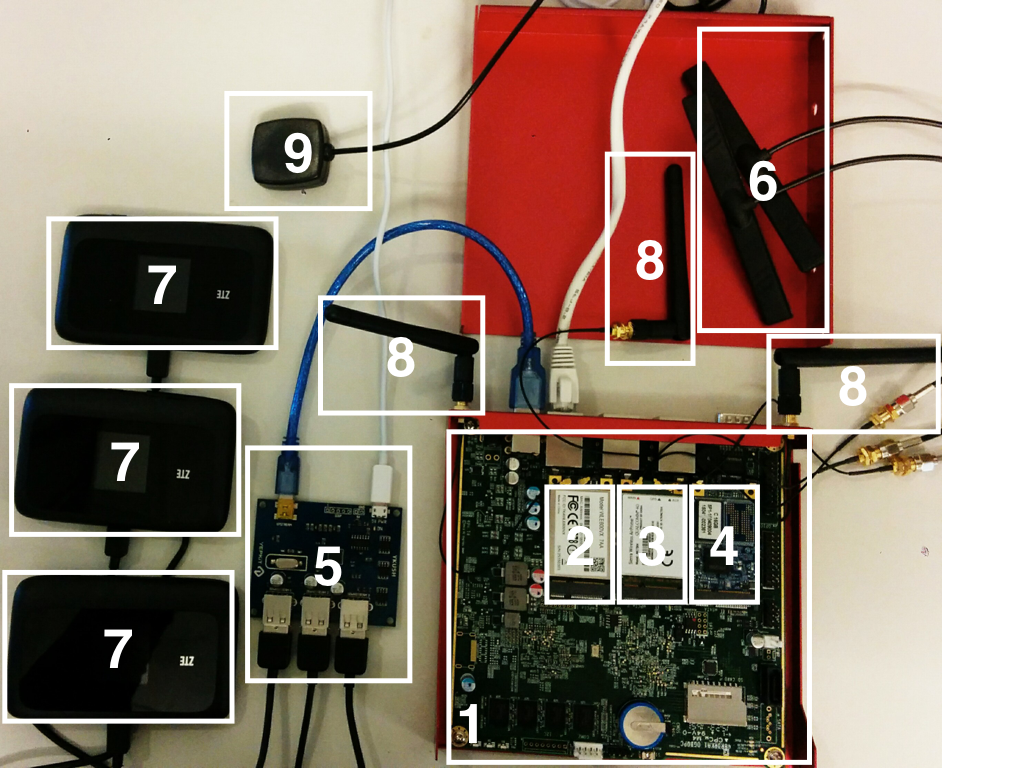
\includegraphics[width=0.75\textwidth]{SystemPicture1.png}
	\caption{First system design. 1) PC Engines APU board. 2) WiFi adaptor. 3) Internal 4G Cat3 Sierra Wireless modem for management. 4) SSD. 5) USB hub. 6) Internal 4G modem antennas. 7) ZTE MF910 LTE Cat4 MiFis. 8) WiFi antennas. 9) GPS antenna.}
	\label{fig:firstNodeDesign}
\end{figure}

\subsubsection{Second design}

The new \monroe{} design presents a heterogeneous set of nodes grouped in pairs:
\begin{itemize*}
	\item ``Head,'' with two Sierra Wireless LTE Cat6 modems.
	\item ``Tail,'' with one Sierra Wireless LTE Cat6 modem and one WiFi adaptor.
\end{itemize*}
Figure~\ref{fig:secondNodeDesign} shows the current node design.
Both types of nodes are based on a PC Engines APU2D4 motherboard with the following characteristics:
\begin{itemize*}
	\item \SI{1}{\giga\hertz} 64-bit quad core AMD Geode APU.
	\item \SI{4}{\gibi\byte} RAM.
	\item \SI{16}{\gibi\byte} SDD.
	\item Three miniPCIe slots, two of which support a 3G/4G modem.
\end{itemize*}

\begin{figure}[tp]
	\centering
	\includegraphics[width=0.75\textwidth]{SystemPicture2.jpg}
	\caption{Second system design. Left: Tail node with one LTE Cat6 modem and one WiFi adaptor. Right: Head node with two LTE Cat6 modems.}
	\label{fig:secondNodeDesign}
\end{figure}

The new node design does not support a dedicated management MBB interface.
Thus, additional measures have been taken to minimize the interference of background traffic with user experiments.
In particular, most maintenance operations (except optionally the transfer of user results) are paused during experiment execution.
Also, a fix hour is reserved for maintenance in all nodes every day.


\subsection{Overview of the node configuration}

\monroe{} nodes have been designed to have minimal impact on the experiments that run on them.
Therefore, only one experiment can run at a given time in a node.
Although the experiments are executed inside a Docker container, they have no quotas on CPU or memory usage, subject only to available node resources.
Container image size and temporary storage in the node may be restricted, though.

Every \monroe{} node runs, in addition to user experiments, the following background processes:

\begin{itemize}
	\item The experiment scheduler, which arbitrates the execution of user experiments in the node.
	The scheduler runs permanently in the background and contacts periodically the scheduling server, sending ``heartbeats'' and checking for new schedules for the node.
	When an experiment is not running, the scheduler may start the deployment of the containers for one or several experiments scheduled to be run in the immediate future, so that they are prepared on advance.
	The scheduler checks the duration of the slot assigned to an experiment; if the experiment does not finish on time, it stops the whole container.
	\item Synchronization (rsync) services to copy data files to the \monroe{} repository.
	This service copies user experiment results, the data collected by passive experiments and assorted metadata measurements.
	It runs continuously, transferring files to the server as they appear in the corresponding folders.
	This service uses the management interface, which is different from the interfaces available for the experiments.
	However, the management interface may share in some cases the same subscriber contract with one of the experiment interfaces; operators might restrict the total bandwidth available for all the SIMs linked to the same contract.
	Additionally, two modems (management plus experiment) using the same operator antenna may somehow affect the bandwidth available for the experiment.
	Therefore, experimenters should be aware of the small amount of data that can be transferred by this service in parallel to their experiments.
	\item Several systems run continuously in the background gathering information on the status of diverse components.
	Examples include a service to read the signal strength and network configuration of each of the experiment modems, the GPS data and various node parameters such as CPU load, memory usage or CPU temperature.
	These services run continuously in the background with a frequency that varies from one second up to several minutes.
	Although their impact on user experiments should be minimal, their existence must be known by the experimenters.
	\item In addition to the services that gather metadata, \monroe{} nodes keep several containers active all the time.
	These containers run experiments that are deemed basic for the \monroe{} platform and include:
	\begin{itemize}
		\item A ping experiment.
		Container number \num{1} executes continuously an ICMP ping operation to a fixed external server (currently, Google's DNS at 8.8.8.8).
		The RTT values are collected and transferred to the servers.
		The ping experiment runs continuously with a frequency of one second, for every interface.
		\item A container that runs Tstat, the passive mPlane monitoring probe that collects, for each interface, detailed flow level statistics.
		The Tstat container generates no traffic; flow level data is synchronized to the \monroe{} repository using the standard synchronization process described above.
	\end{itemize}
	\item Finally, some built-in \monroe{} experiments run as scheduled containers.
	These experiments will not run at the same time than user experiments:
	\begin{itemize}
		\item A bandwidth measurement test, which periodically downloads an object using the HTTP protocol to measure the achievable bandwidth.
		The test runs on each interface.
		The periodicity of this experiment and whether it can be run while user experiments are being executed are yet to be decided.
		\item A container that periodically executes a paris-traceroute to several popular websites recording information about all the intermediate hops.
		This container will in principle be run several times per day, but the interactions with user experiments are yet to be determined.
	\end{itemize}
\end{itemize}

\subsection{Overview of the experimental workflow}

Experiments conducted in the \monroe{} platform follow the workflow shown in Figure~\ref{fig:ExperimentWorkflow}, which consists of three phases: Experiment design, testing and experimentation.
During the experiment design phase, the experiment goals and properties are defined and the container required to deploy it in \monroe{} nodes is configured.
During the testing phase, the container is executed on nodes specifically devoted to testing new experiments.
If the experiment passes all the safety and behavior tests, a \monroe{} manager will digitally sign the container image.
Signed containers cannot be further modified without running again through the testing phase.
Finaly, the experimenter is free to schedule the experiment container on any nodes, subject to the specific quotas assigned to their project.

\begin{figure}[tp]
	\centering
	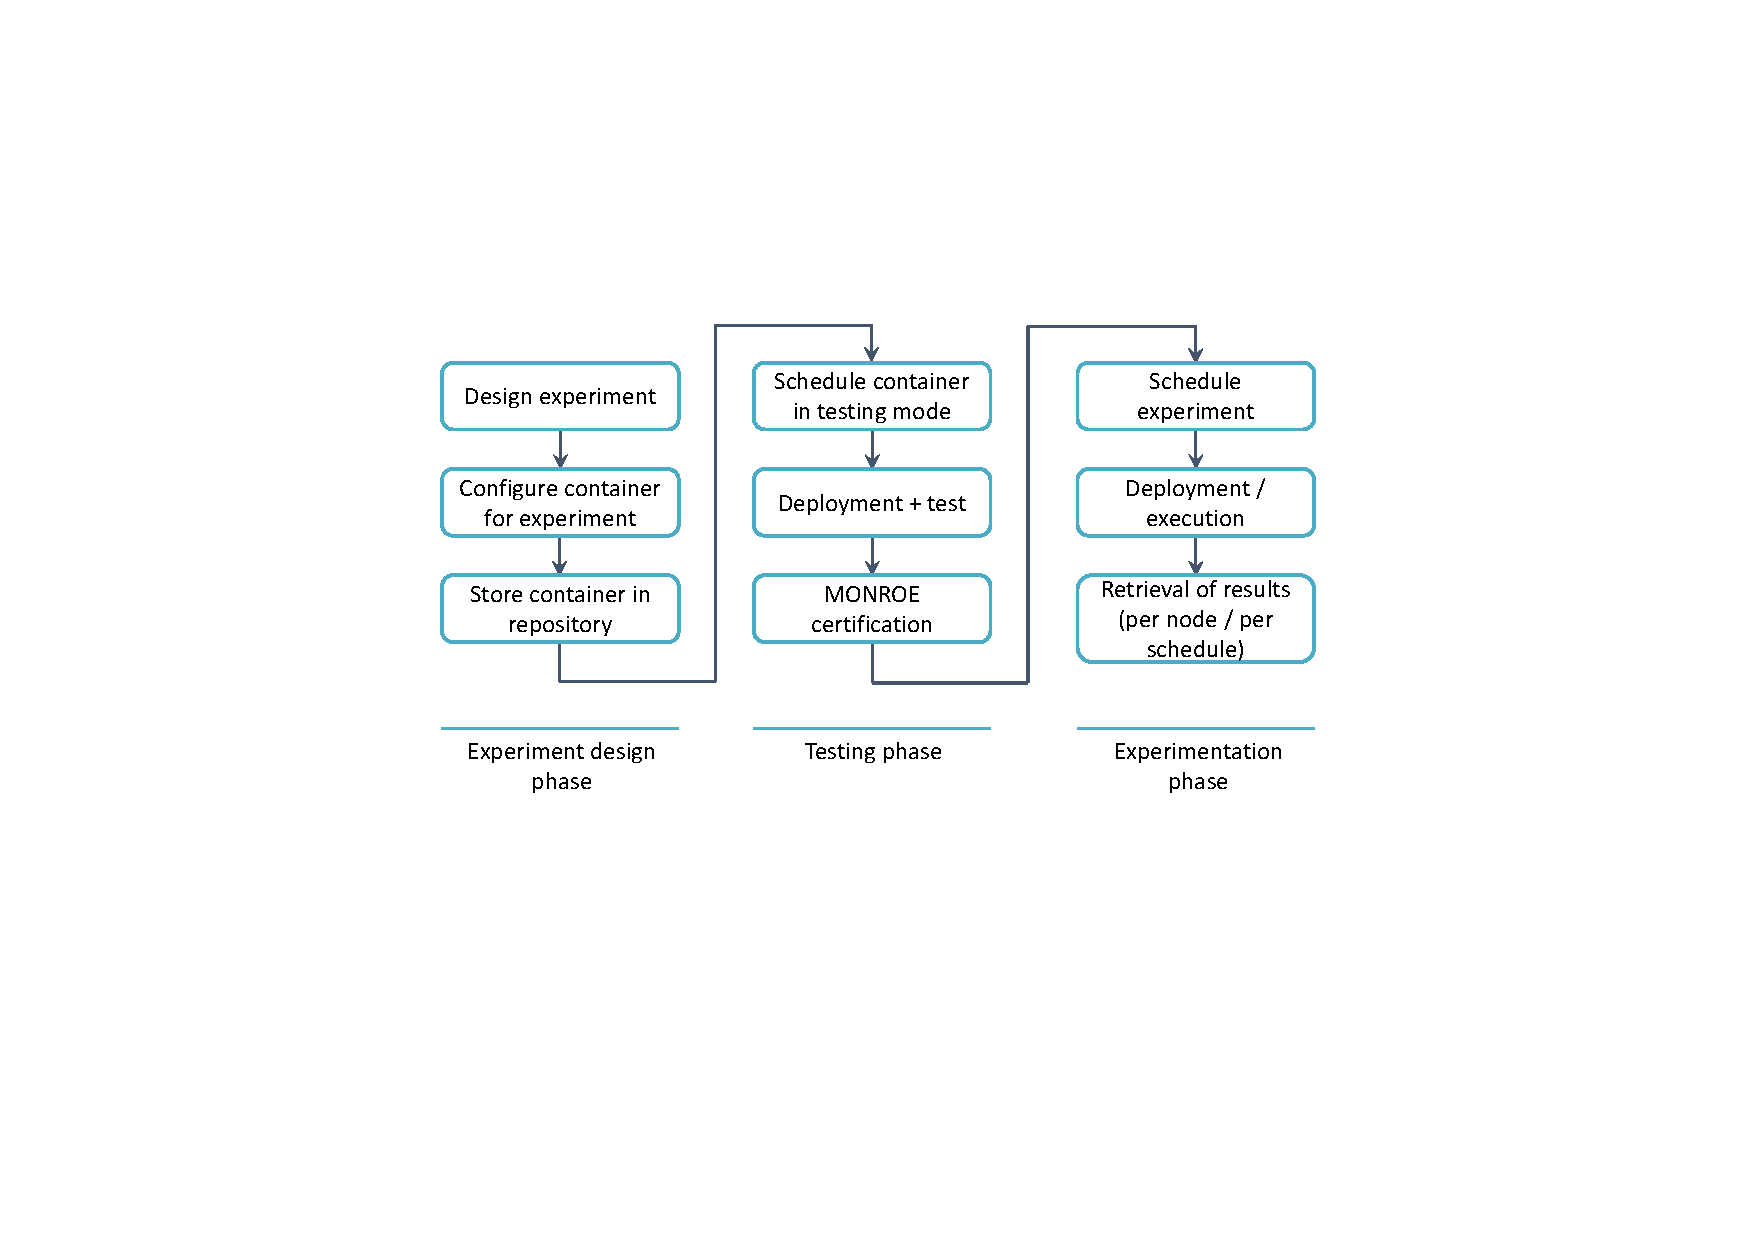
\includegraphics[width=1.0\textwidth,trim={7cm 7.5cm 7cm 5cm}]{ExperimentWorkflow.pdf}
	\caption{Experimental workflow.}
	\label{fig:ExperimentWorkflow}
\end{figure}


%------------------------------------------------------------%
%------------------------------------------------------------%
%------------------------------------------------------------%

\section{Experiment preparation}
\label{sec:experimentPreparation}

%Abcd.

\subsection{General experiment notes}
\label{subsec:generalExperimentNotes}

\monroe{} experiments run under the root user of a Docker container.
Therefore, experimenters can design any kind of experiment within the security restrictions of the platform, including the configuration of routing tables, stopping or starting interfaces and executing any kind of applications.
We assume the reader is familiar with the Docker technology.
Otherwise, we suggest getting used to it by accessing the documentation at \url{https://docs.docker.com/engine/understanding-docker/}~.

Creating and using containers is a two-step process.
At design time, the experimenters create the image for the container in their local machine using a container-creation script.
If necessary, they can install new packages (e.g., via apt-get) or copy libraries.
The docker tools read the script and create the final image for the experiment, which will then have to be uploaded to a repository.
At run-time, the nodes retrieve the container image from the repository and start it as scheduled.

During execution, the experiment should not install additional applications or download any data that is not part of the experiment itself (e.g., if the experiment uploads a file to a server to test upstream speed, either include the file to be uploaded in the container at design time or create it locally).

\emph{$\Rightarrow$~Experiments will under no circumstances allow direct ssh access to the node or any other form of running interactive commands from outside the container that can pose a security risk for the platform.~$\Leftarrow$}

\subsection{Container preparation}
\label{subsec:containerPreparation}

\monroe{} experiments are deployed in Docker containers (\url{https://www.docker.com/}).
Preparing a new container from \monroe{}'s base image is an easy process:

\begin{enumerate}
	\item Install Docker in your machine. Do it preferably downloading the installation script  from the web page, rather than through a package manager such as apt-get:
		{\VerbatimFont\begin{verbatim}
			$ wget https://get.docker.com -O install.sh
			$ chmod u+x install.sh
			$ ./install.sh
		\end{verbatim}}
		You will have to run docker as root unless you add yourself to the docker group.

		Mac users: Download and install ``Docker for MAC''\\
		(\url{https://www.docker.com/products/docker#/mac})\\
		or the ``Docker Toolbox''\\ (\url{https://docs.docker.com/toolbox/overview/}), according to your OS version.
	\item Test the Docker installation with the `Hello world!' example:
		{\VerbatimFont\begin{verbatim}
			$ sudo docker run hello-world
			Unable to find image 'hello-world:latest' locally
			latest: Pulling from library/hello-world
			03f4658f8b78: Pull complete
			a3ed95caeb02: Pull complete
			Digest: sha256:xxxxxxxxxxxxxxxxxxxxxxxx
			Status: Downloaded newer image for hello-world:latest
		\end{verbatim}}
		If everything has worked correctly up to here, you will see a welcome message similar to the following:
		{\VerbatimFont\begin{verbatim}
			Hello from Docker.
			This message shows that your installation appears to be working correctly.
			...
		\end{verbatim}}
		You can check which images are locally installed with:
		{\VerbatimFont\begin{verbatim}
			$sudo docker images
			REPOSITORY    TAG      IMAGE ID       CREATED        SIZE
			hello-world   latest   690ed74de00f   4 months ago   960 B
		\end{verbatim}}
  \item Now you are ready to download the \monroe{} base image:
		{\VerbatimFont\begin{verbatim}
			git clone https://github.com/MONROE-PROJECT/Experiments.git
		\end{verbatim}}
		This will fetch the repository with \monroe{}'s example containers.
	\item Head to \identifier{Experiments/experiments/template/}.
		Here, you will find the required files to prepare your image based on \monroe{}'s base.
		You should care about four things: a) The contents of the \identifier{files/} folder, b) the \identifier{build.sh} file, c) the \identifier{push.sh} file and d) the \identifier{template.docker} script file that describes how to create your container.
		In the directory \identifier{files/} you can put all the files that are part of your experiment.
		As a simple example, we can use the following script:
		{\VerbatimFont\begin{verbatim}
			$vi files/myscript.sh
			  #!/bin/bash
			  ls -lah > /monroe/results/listing.txt
		\end{verbatim}}
		Any files that your experiment creates in \identifier{/monroe/results} are delivered to the repository, where you will be able to retrieve them.
		\emph{Writes to any other part of the filesystem will be lost once the experiment is finished.}
		In periodic schedules, no data will survive from one execution to the next (i.e., the container is loaded fresh before each execution).
		If result persistence is needed, the experimenter will have to supply it by downloading the needed files from the network during the experiment itself.
	\item You should not need to modify the \identifier{build.sh} file. The name of the container is the name of the current directory, and it must match the name of the \identifier{.docker} file (e.g., \identifier{template.docker} as we are in a folder named \identifier{template/}).
	
	\item The file \identifier{template.docker} is the script used to build your container.
		You can modify it to:
		\begin{itemize}
			\item Define the entry point of your experiment (``ENTRYPOINT'').
			\item Change the base image of the container, e.g., \identifier{monroe/base}.
			\item Install additional packages or libraries.
		\end{itemize}
		For example:
		{\VerbatimFont\begin{verbatim}
			FROM monroe/base
		
			MAINTAINER your-email-address
		
			COPY files/* /opt/monroe/
		
			#Default cmd to run.
			ENTRYPOINT ["dumb-init", "--", "/bin/bash", "/opt/monroe/myscript.sh"]
		\end{verbatim}}
	
		This example will copy the files in the \identifier{files/} directory to the one you specify \emph{inside} the docker container (e.g., \identifier{/opt/monroe}).
		
		TIP: If you need to install additional packages in the container, be sure to clean any temporary files from the image. Also, notice that the Docker creation script analyses the contents of the container filesystem after every line in the .docker script is executed. That means that, even if you delete files at the end, Docker will create intermediate ``layers'' that will be downloaded and applied sequentially to build the final image of your container. Consider instead using one-liners such as the following:
		{\VerbatimFont\begin{verbatim}
		    RUN apt-get update && apt-get install -y vim && apt-get clean
		\end{verbatim}}
		This will ensure that the files are deleted before Docker analyses the filesystem.
	\item Modify the file \identifier{push.sh} to reflect the name of your repository:
		{\VerbatimFont\begin{verbatim}
			#!/bin/bash
			DIR="$( cd "$( dirname "${BASH_SOURCE[0]}" )" && pwd )"
			
			CONTAINER=${DIR##*/}
			
			CONTAINERTAG=myuser/myrepo # --> Modify to your own dockerhub user/repo
			
			docker login && docker tag ${CONTAINER} ${CONTAINERTAG} && docker push ${CONTAINERTAG} && \
			    echo "Finished uploading ${CONTAINERTAG}"					
		\end{verbatim}}
		During the development phase of your experiment, follow these steps to make your container accessible for the testing nodes:
		\begin{itemize}
			\item Create an account at Docker Hub.
			\item Create a private repository (you can create one container as private; no limits for public ones).
			\item In your development machine, run: \identifier{docker login}. It will ask you for your credentials.
		\end{itemize}
	\item After populating the \identifier{files/} directory, modifying the .docker file and updating the \identifier{push.sh} file, you are ready to create the image:
		{\VerbatimFont\begin{verbatim}
			$sudo ./build.sh
			Using default tag: latest
			latest: Pulling from monroe/base
			Digest: sha256:6df1195a3cc3da2bfe70663157fddc42e174ec88761ead7c9a3af591e80ebbd5
			Status: Image is up to date for monroe/base:latest
			Sending build context to Docker daemon 11.26 kB
			Step 1 : FROM monroe/base
			---> d1b4f4baa60d
			Step 2 : MAINTAINER mikepeon@imdea.org
			---> Using cache
			---> 0b05b5c453c7
			Step 3 : COPY files/* /opt/monroe/
			---> acc2df443070
			Removing intermediate container 66a666516a27
			Step 4 : ENTRYPOINT dumb-init -- /bin/bash /opt/monroe/myscript.sh
			---> Running in f4b7a1ee804a
			---> 096c7a56ff1c
			Removing intermediate container f4b7a1ee804a
			Successfully built 096c7a56ff1c
			Finished building template
		\end{verbatim}}
	\item Test that your new docker container is available:
		{\VerbatimFont\begin{verbatim}
			$sudo docker images
			REPOSITORY                                   TAG    IMAGE ID      CREATED         SIZE
			hello-world                                  latest 690ed74de00f  4 months ago    960 B
			your_docker_account/your_experiment          latest xxxxxxxxxxxx  32 seconds ago  626.6 MB
			monroe/base                                  latest xxxxxxxxxxxx  12 days ago     626.6 MB
		\end{verbatim}}
		Exact image ids and sizes will vary.
	\item Push the container image to the repository:
		{\VerbatimFont\begin{verbatim}
			$ sudo ./push.sh
			Username (your-Docker-user-name):
			Password: (type your DockerHub password)
			WARNING: login credentials saved in /home/your-username/.docker/config.json
			Login Succeeded
			The push refers to a repository [docker.io/mikepeon/template]
			5f339bfdaae2: Pushed
			486ab26686cc: Layer already exists
			034f70c0d9cd: Layer already exists
			86b5acd8772a: Layer already exists
			f03317610243: Layer already exists
			50f6c1bd7ce6: Layer already exists
			aec5953bffa2: Layer already exists
			507169b05eea: Layer already exists
			5d799297d10c: Layer already exists
			759d76df9ac7: Layer already exists
			5f70bf18a086: Layer already exists
			12e469267d21: Layer already exists
			latest: digest: sha256:c855de65307191b4832b2ec60a4401c1b63424827c29149703c5d7ef07b519f7
			size: 3001
			Finished uploading your-username/template
		\end{verbatim}}
	\item You can now test that your image runs correctly, even on your own PC (if the experiment logic and resource demands allow for it).
		{\VerbatimFont\begin{verbatim}
			$mkdir /run/shm/myresults
			$sudo docker run -v /run/shm/myresults:/monroe/results your_docker_account/your_experiment
			    --> The output of your experiment will be in /run/shm/myresults/listing.txt
		\end{verbatim}}
		The docker command line allows you to specify a mapping between a directory inside the docker image and one in the host system.
		In this case, we have mapped \identifier{/monroe/results} from the container to \identifier{/run/shm/my\-results}.
		This is useful if you are running the container locally in a normal PC for debugging purposes.
		
		\textbf{IMPORTANT:} This process shows how to build and run a container \emph{locally} in your workstation.
		However, experimenters do not have direct access to the \monroe{} nodes.
		Therefore, to execute your experiment \emph{in} a \monroe{} node, you will follow the process just up to the \identifier{sudo ./push.sh} step and then use the web interface to upload and schedule the container into the nodes.
\end{enumerate}

You may check the contents of \identifier{experiments/*} for more useful examples.

The following is a list of useful common Docker commands:
\begin{itemize*}
	\item To list installed/built images (and get their ids):
	\begin{verbatim}docker images\end{verbatim}
	\item To list running containers and get their tags:
	\begin{verbatim}docker ps\end{verbatim}
	\item To stop running containers:
	\begin{verbatim}docker kill container-tag\end{verbatim}
	\item To delete images:
	\begin{verbatim}docker rm -f image_id\end{verbatim}
	\item To retrieve the latest version of an image (e.g., \identifier{monroe/base}):
	\begin{verbatim}docker pull monroe/base\end{verbatim}
	\item To attach to a running container and get an interactive shell:
	\begin{verbatim}docker exec -i -t container-tag bash\end{verbatim}
\end{itemize*}

\subsubsection{Package and tool installation}
\label{subsubsec:packagesInstallation}

If you have to install extra packages, libraries or tools, do it from the \identifier{my\_experiment.docker} file.
You should never pull repositories or download libraries from inside your experiment as this will count against your data quota (and execution slot) for every instance of your experiment.
Instead, modify the container configuration file as in the following example:
{\VerbatimFont\begin{verbatim}
			FROM monroe/base
			
			MAINTAINER your-email-address
			
			RUN apt-get update && apt-get install -y \
			    python \
			    python-pip \
			    traceroute \
			    && apt-get clean
			RUN pip install pygame
			
			RUN mkdir -p /opt/yourname
			COPY files/* /opt/yourname/
			
			#Default cmd to run
			ENTRYPOINT ["dumb-init", "--", "/bin/bash", "/opt/yourname/myscript.sh"]
\end{verbatim}}

You may also download any files using \identifier{wget}, but you may simply put them in the \identifier{files/} folder as well.
Remember, this happens during container creation on your PC, \emph{not} during experiment execution on the nodes.

If you find the need for big libraries that you think should go into the base image, please contact \monroe{}'s administrators.

TIP: The easiest way to find out which packages and versions are available in the \monroe{} base image is to create a simple container and run an interactive batch session inside it in your workstation.
For example, assuming that you have a basic container that simply waits when run, you may follow the following steps:
{\VerbatimFont\begin{verbatim}
	mkdir /run/shm/myresults
	docker run -v /run/shm/myresults:/monroe/results repository/your_container &
	docker ps --> Look for the tag of your running container
	docker exec -i -t container_tag bash
	--> Here you are inside the container
	dpkg -l > /monroe/results/package-listing.txt
	exit
	--> You'll find the output at /run/shm/myresults/package-listing.txt
\end{verbatim}}
For easier reference, Table~\ref{tab:installedPackages} in Appendix~\ref{app:installedPackages} gives a detailed listing of packages available in \identifier{monroe/base} at the time of writing this text.

\subsection{Optional interactive debugging}
To speed up the process of debugging experiments in the nodes, three debugging paths are provided.

First, experimenters can order (buy) a number of ``development'' nodes to be hosted locally in their premises.
These nodes, which will not be accessible through the standard scheduler and user interface, can be accessed through local interfaces (eth, serial console) and provide root access.

Second, and only for ``testing'' nodes, the user interface includes an option to provide an SSH public key to the container.
Once the container starts, experimenters can connect to monitor experiment progress.
The SSH session can extend until the container finishes or is stopped.

Finally, a virtual machine containing a ``virtual \monroe{} node'' has been designed to ease development and debugging on a local PC.
This virtual node replays metadata previously recorded from a real one.

\subsection{Mandatory certification process}
\label{subsec:testingProcess}
\monroe{} experiments have to be certified before they can be executed by deployed nodes.
A small number of nodes are available through the user interface so that experimenters can test their experiments before starting the certification process.

The certification process consists of the following steps:
\begin{enumerate}
	\item The experimenter contacts their patron to inform them that a new version of their experiment is ready for certification.
	
	\item The experimenter has to provide a summary of the experiment, i.e., overall purpose, design and implementation (reasonable length around \num{0.5} to \num{1} A4~pages).
	
	\item The container should be submitted as source (i.e., build scripts for Docker, not tools source code) for easy inspection by the patron.
	Additionally, this will allow the \monroe{} administrators to update the containers when a new version of \identifier{monroe/base} is available.
	
	\item The patron, or the maintenance team, will then build (or pull) the container, tag it as \identifier{partnername/\allowbreak experimentname}, and push it to the deployed docker repository.
\end{enumerate}

Every experiment submitted to the \monroe{} testbed \emph{must} first pass through a testing process to receive manual approval by a \monroe{} administrator.
To submit your experiment for testing, you have to use the web interface specifying ``testing'' as the required node type.

\subsection{Deployment}
\label{subsec:deployment}
\monroe{}'s scheduling system will automatically deploy experiments to the nodes before their execution time.
The nodes will fetch the container image from the Docker repository, and the size of the download will be accounted in your data quota.
Notice that in the case of periodic experiments, each time an experiment is run, the Docker container may have to be re-downloaded and its costs will be accounted in your quota.

\subsection{Life cycle of monroe/base}

The current version of \identifier{monroe/base} deployed on nodes is tagged as ``latest.''
New versions will be tagged as ``staging;'' their existence will be announced on the experimenters mail list.
Experimenters must check their experiments against the new stagging version to verify that no incompatibilities appear.
Any relevant issues can be discussed with the \monroe{} administrators.
After a reasonable period of time, the new version will be retagged as ``latest,'' and deployed into the nodes.
All the containers should have been built against the new version at this time to avoid wasting quota resources when they are deployed in the nodes.


%------------------------------------------------------------%
%------------------------------------------------------------%
%------------------------------------------------------------%

\section{Resource allocation, and experiment scheduling and monitoring}
\label{sec:allocSchedMonitor}

Once a experiment is configured as a Docker container, it can be scheduled multiple times under different conditions using the user client web located at \url{https://www.monroe-system.eu}~.

\subsection{User login and certificates}
\label{subsec:login}
User identification in \monroe{} is achieved through client certificates.
Every experimenter has their own certificate compatible with the FED4FIRE%
\footnote{\url{http://www.fed4fire.eu/}} %
federation.
User certificates are issued by iMinds through the following URL: \url{https://authority.ilabt.iminds.be/}.
New users must create a new account (``sign up'').
Be sure to select the option ``Join Existing Project'' and type the name ``Monroe'' in the project name field (Figure~\ref{fig:iMindsCreateAccount}).
The authorization process involves a manual verification step by one of the \monroe{} administrators, so it will probably take one or two days.

\begin{figure}[tp]
	\centering
	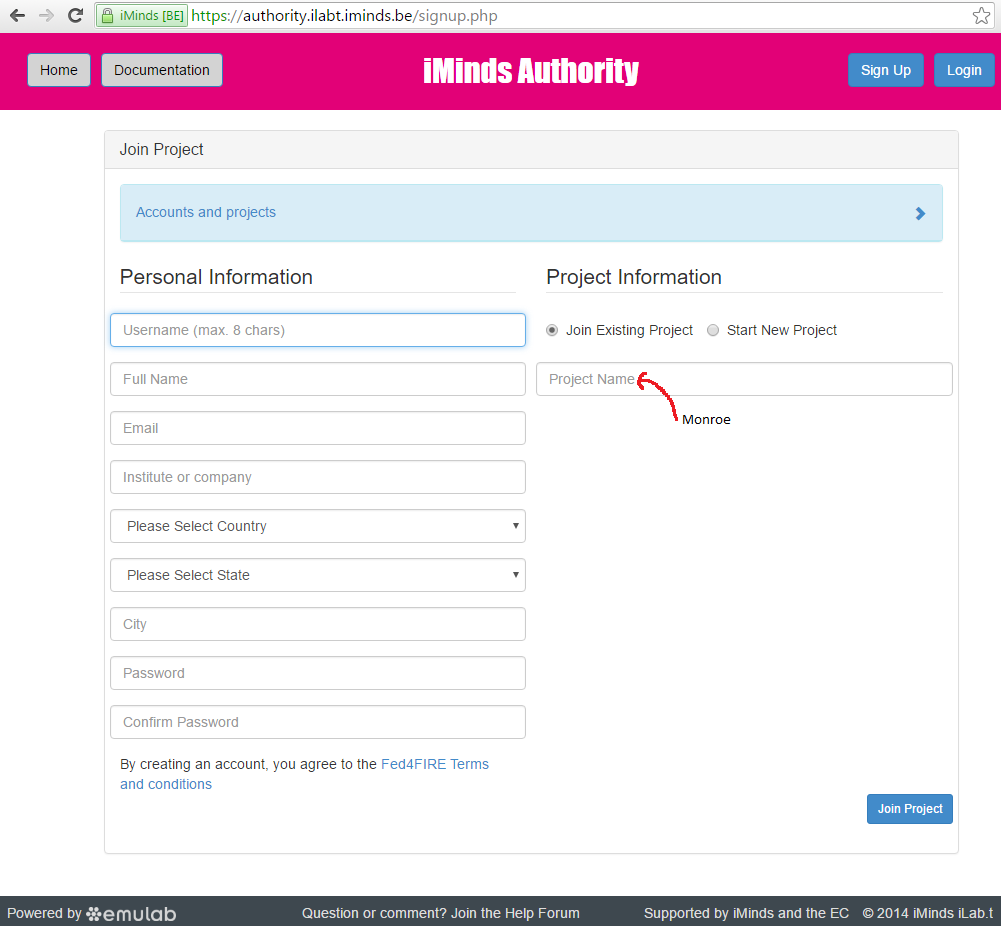
\includegraphics[width=0.5\textwidth]{iMindsCreateAccount2.png}
	\caption{iMinds registration page to obtain FED4FIRE-compatible certificates for use with the \monroe{} platform.}
	\label{fig:iMindsCreateAccount}
\end{figure}

Please, notice that the current policy for \monroe{} is to use one user certificate per project, shared between all the experimenters belonging to that project.

Once the identity of the experimenter is approved, they will receive an informative email.
They should then log into the iMinds webpage to download the certificate files (PKCS12).
These files must be installed in the experimenter browser.
After that, the user should be able to access the user web directly.
Upon request of the main (index.html) file, the browser will contact \monroe{} servers to verify that the user credentials are correct.
In the case of any problems, the user will be presented with instructions on how to obtain a certificate.
If the client certificate is verified successfully, they will be automatically redirected to the listing of their experiments.

\textbf{NOTE:} User certificates are manually activated in the scheduling software.
To use your certificate, please send its SSL ID (``fingerprint'') to one of the \monroe{} administrators (e.g., \url{mailto:mikepeon@imdea.org}).
You may find it in the screen after pressing the ``Try me'' button, once the certificate is correctly installed in your browser:
{\VerbatimFont\begin{verbatim}
{
"fingerprint": "c79f1967aea17811a1ebed39b7d718430904338a",
"user": {
    "id": 3,
    "name": "MONROE Test admin",
    "quota_data": 50000000000,
    "quota_storage": 500000000,
    "quota_time": 500000000,
    "role": "admin",
\end{verbatim}
\color{red}
\vspace{-0.7cm}
\begin{verbatim}
    "ssl_id": "c79f1967aea17811a1ebed39b7d718430904338a"
\end{verbatim}
\color{black}
\vspace{-0.7cm}
\begin{verbatim}
},
"verified": "SUCCESS"
}
\end{verbatim}}

~\\$\Rightarrow$~We have identified some common issues that are not yet solved. Below are some workarounds:
\begin{itemize}
	\item For the first login, you may be asked for your user certificate and then your browser may show a security warning. This is due to the use of a self-signed server certificate. Please ask your browser to proceed. Then, you will probably see an error page from \monroe{}. Please, click the red button labeled ``Try me'' and check that you get a successful data output. Finally, please proceed again to the main page of the project. From that point, you should be able to access the system without further problems in future sessions. (Pointers on how to simplify this issue are welcome!)
	\item Firefox on OSX has an issue with CORS headers. Although the web and scheduling servers are running now on the same machine, you may still encounter this problem.
\end{itemize}

\subsubsection{Installation of user certificates in Chrome}
\label{subsec:userCertsInstallWinChrome}

This section explains how to install the FED4FIRE-compatible user certificates used by the \monroe{} platform in Google Chrome for Windows.
The procedure for other browsers and platforms should be similar.

\begin{enumerate}
	\item Go to your browser settings page:\\
	\begin{center}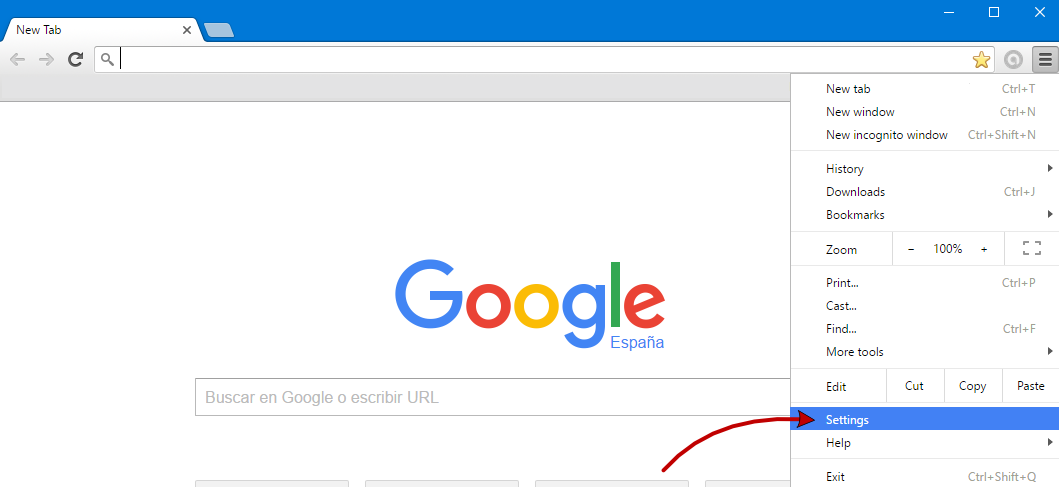
\includegraphics[width=0.7\textwidth]{InstallCert01.png}\end{center}
	
	\item Display the advanced configuration settings:\\
	\begin{center}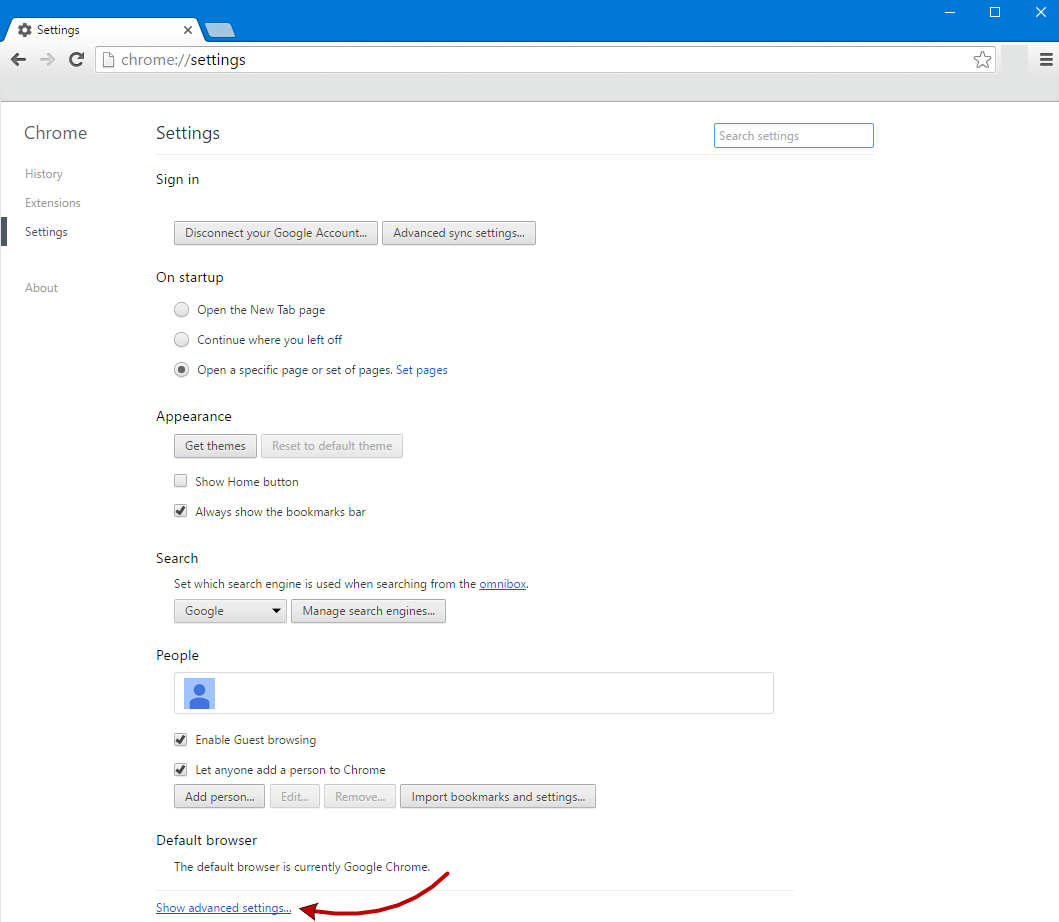
\includegraphics[width=0.7\textwidth]{InstallCert02.png}\end{center}
	
	\item Go to the section labeled ``HTTPS/SSL'' and click the button ``Manage certificates...'':\\
	\begin{center}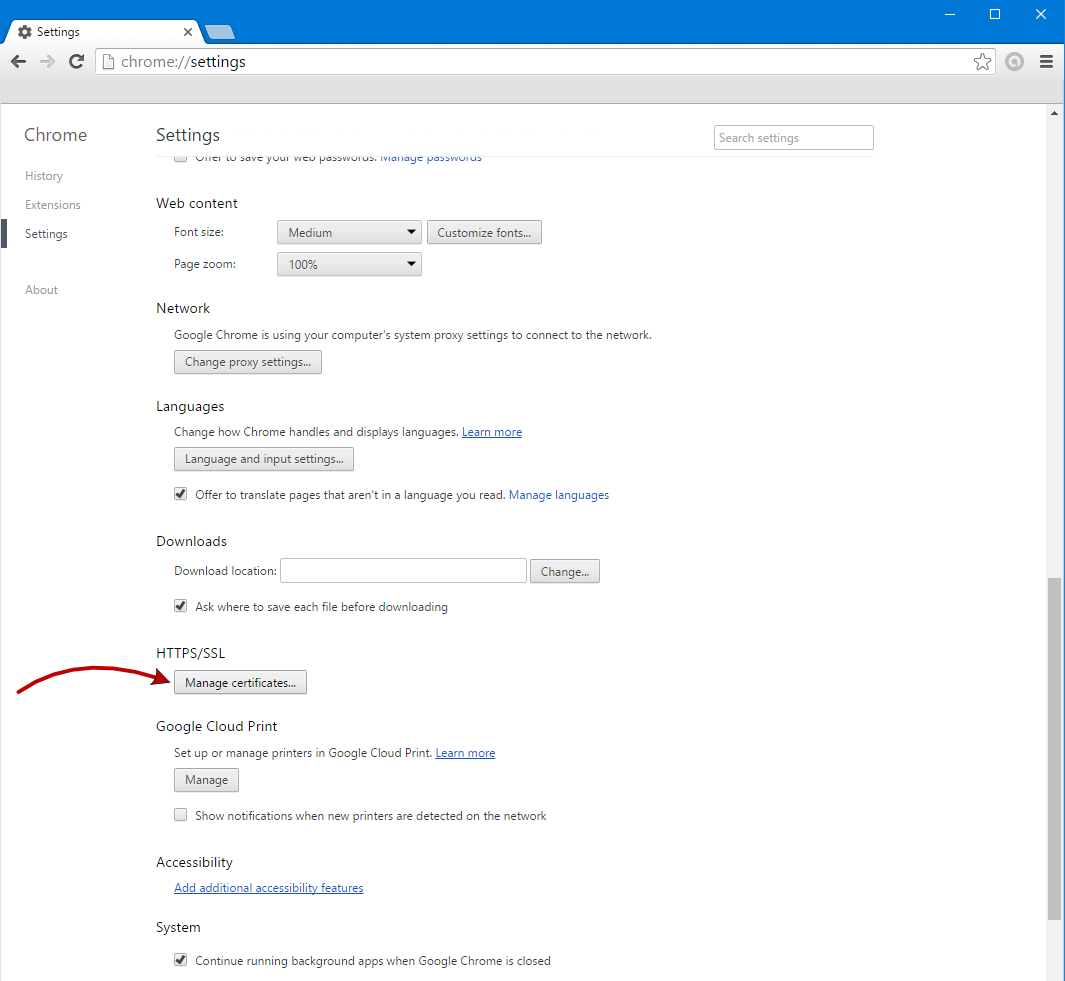
\includegraphics[width=0.7\textwidth]{InstallCert03.png}\end{center}
	
	\item The dialog box for managing your certificates will be displayed. Press the button ``Import...'' to import your certificate:\\
	\begin{center}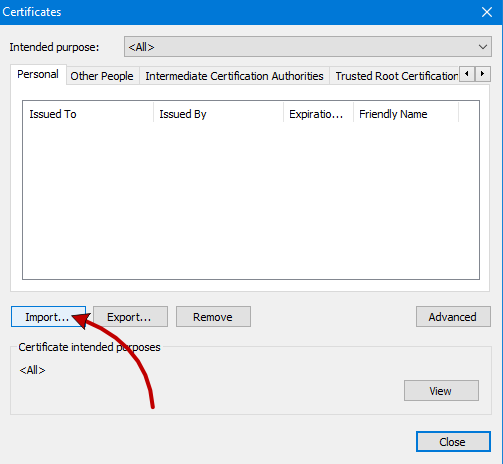
\includegraphics[width=0.5\textwidth]{InstallCert04.png}\end{center}
	
	\item In the new dialog, click ``Next'':\\
	\begin{center}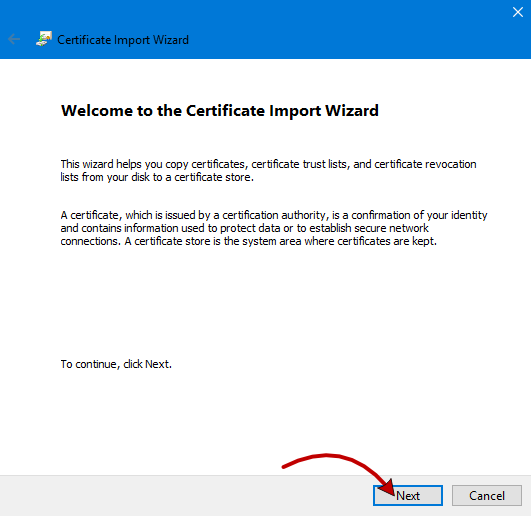
\includegraphics[width=0.5\textwidth]{InstallCert05.png}\end{center}
	
	\item In the file-selection dialog that appears next, change the file type from ``X.509 Certificate (*,cer;*.crt)'' to ``Personal Information Exchange'':\\
	\begin{center}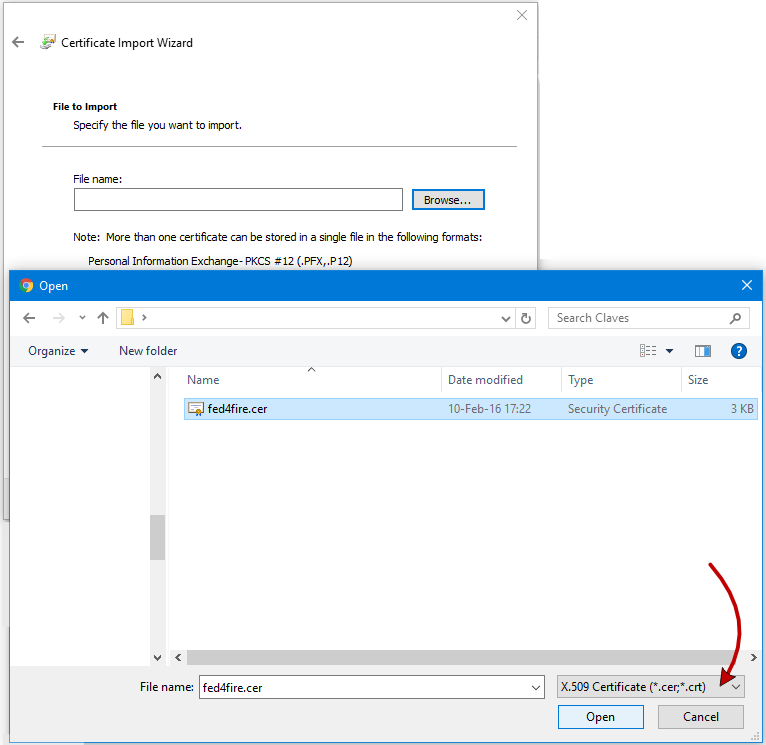
\includegraphics[width=0.6\textwidth]{InstallCert06.png}\end{center}
	
	\item And select the file containing your certificate:\\
	\begin{center}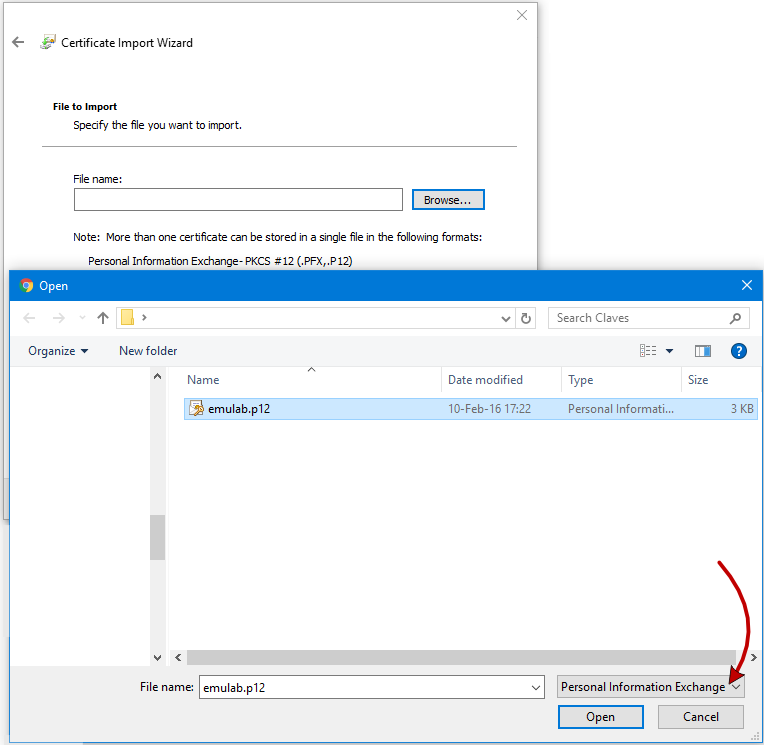
\includegraphics[width=0.6\textwidth]{InstallCert07.png}\end{center}
	
	\item In the next dialog box, enter your certificate password:\\
	\begin{center}\centering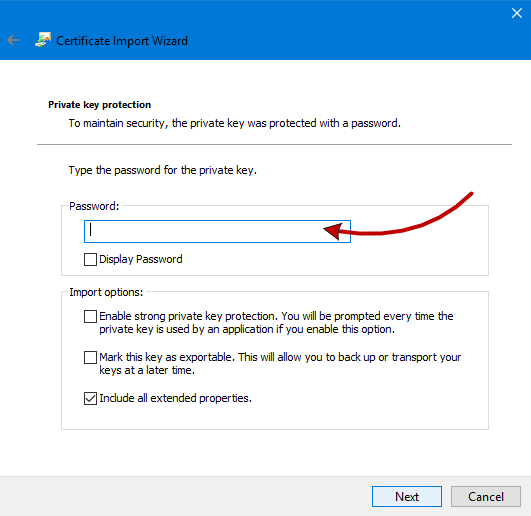
\includegraphics[width=0.5\textwidth]{InstallCert08.png}\end{center}
	
	\item If the import is successful, your certificate will be imported to your ``Personal Store'' and you will be able to access the \monroe{} user interface by selecting it when prompted by your browser. Notice that you may still get a warning about the validity of the server certificate.
	
\end{enumerate}

\FloatBarrier
\subsection{Resource allocation}
\label{subsec:resourceAllocation}
The ``New'' tab allows assigning resources and scheduling new experiments.
Here, the user will be presented with a page similar to Figure~\ref{fig:newExperimentBlank}.

\begin{figure}[tp]
	\centering
	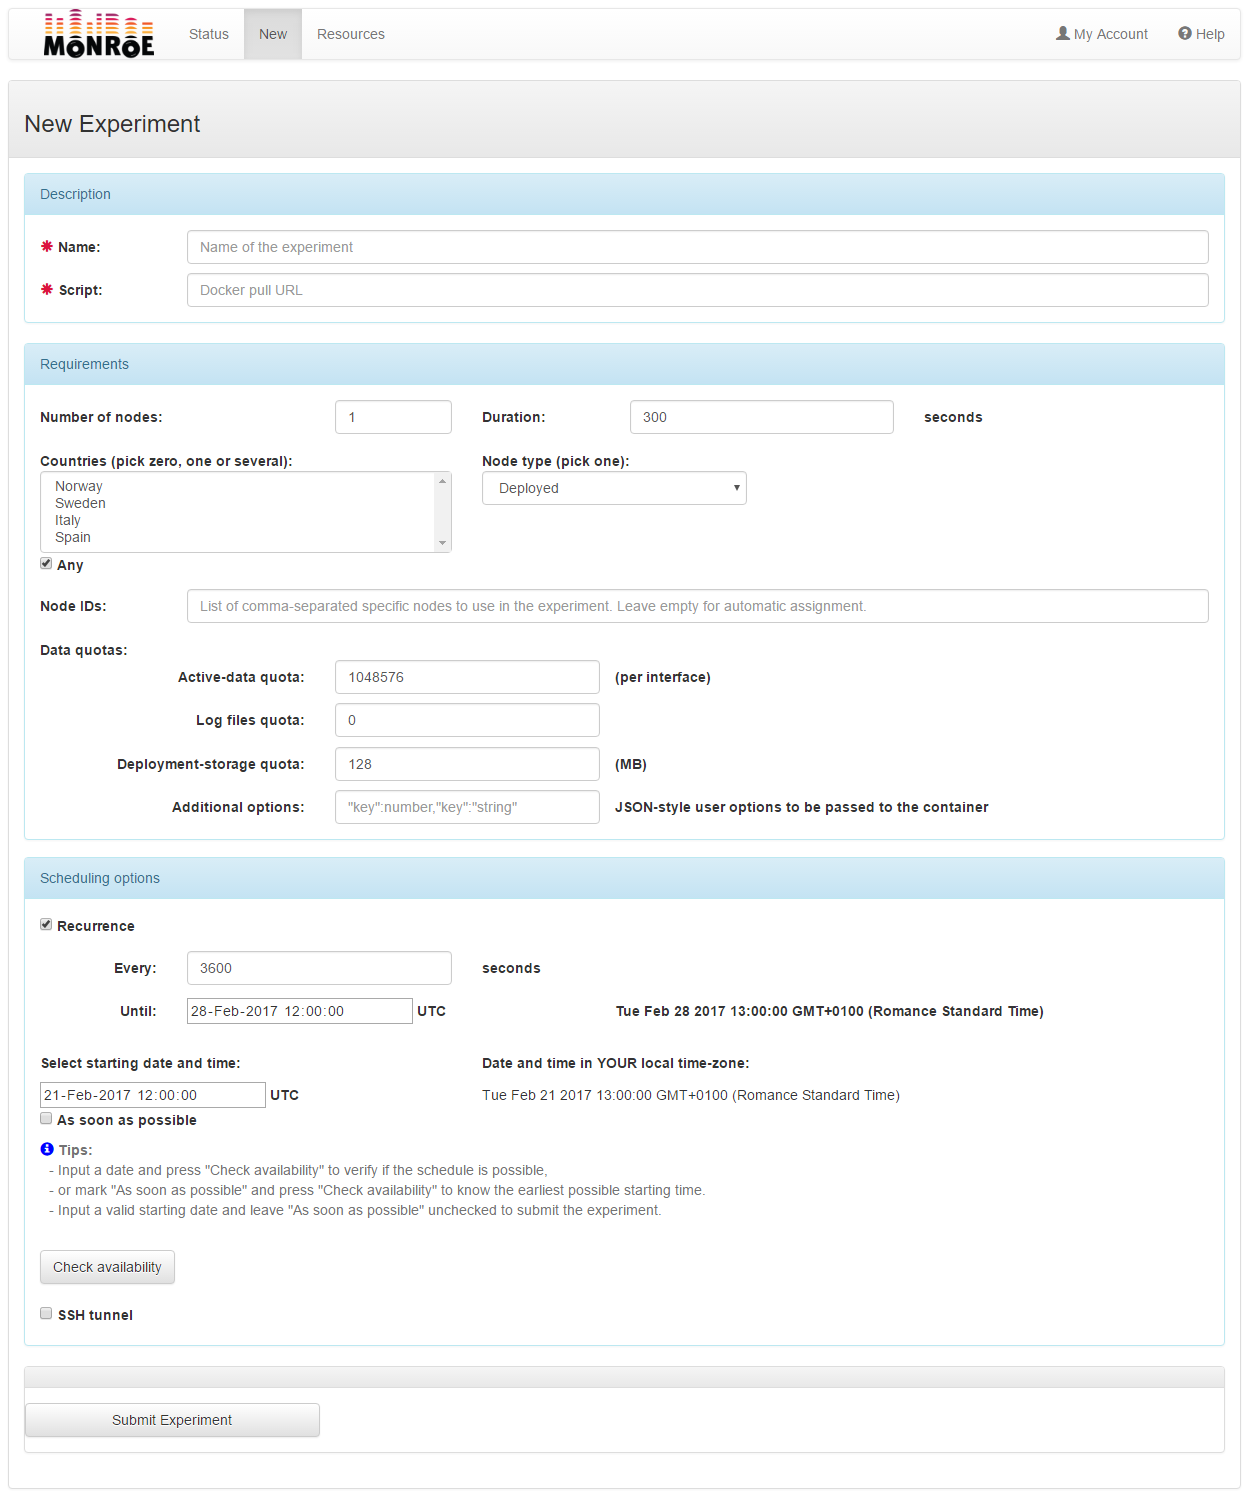
\includegraphics[width=1.0\textwidth]{NewExperiment_blank.png}
	\caption{Example for the creation of a new experiment.}
	\label{fig:newExperimentBlank}
\end{figure}

To create a new experiment, at least the following parameters must be specified:
\begin{description}
	\item [Name:] A representative experiment description.
	\item [Script:] A Docker hub path for the experiment container. In the previous example, it would be \identifier{your\_\allowbreak docker\_\allowbreak account/my\_\allowbreak experiment.} Experiments on deployed nodes must be lodged in \monroe{}'s repository: \identifier{monroe1.cs.kau.se:5000/my\_experiment}.
	\item [Number of nodes:] The number of nodes that must execute the experiment.
	\item [Duration:] Length of the experiment execution, in seconds (excluding the time required to deploy the container).
	The node will kill the experiment after this time. The minimum slot that can be reserved is $\SI{5}{\minute}$ and the maximum, $\SI{24}{\hour}$. However, because of the scheduling of \monroe{} experiments, the maximum possible duration is in practice slightly less than three hours.
\end{description}

If the starting date is fixed, the user can introduce it in the field ``Start.''
All dates are introduced as UTC times; the interface presents alongside the corresponding local time for the user's browser.
The scheduler will then try to satisfy the requirements.

Alternatively, if the starting date is not relevant, the user may leave this field empty and press the button ``Check availability'' to check the earliest available slot (add at least ten minutes to the proposed time to allow for container deployment into the nodes).
If the user just wants to submit the experiment as soon as possible, they can just mark the option ``As soon as possible'' and leave the other fields empty when pressing the ``Submit'' button.

Additionally, the user may specify the following restrictions (Figure~\ref{fig:newExperimentFilters}):
\begin{description}
	\item [Country filter:] The user may select nodes located in one or several countries, or they may choose to use nodes from any country indistinctly.
	\item [Node type:] %Available node types are static or mobile (e.g., in buses or trains).
	%Some mobile nodes may have restricted availability.
	%The ``testing'' nodes are reserved for experiments that must still be sanctioned by a \monroe{} administrator.
	Currently available node types are deployed or testing.
	The testing nodes are reserved for experiments that must still be verified by a \monroe{} administrator.
	Experiments on deployed nodes must be lodged in \monroe{}'s repository: \identifier{monroe1.cs.kau.se:5000/}.
	\item [Node model:] Until complete retirement of the old \monroe{} nodes, experiments can run on old or new nodes. Eventually, all experiments will be run on new nodes.
	\item [Number of interfaces:] New \monroe{} nodes come in pairs of co-located nodes, where one node (``head'') has two 4G interfaces, and the other (``tail'') has one 4G interface and one WiFi interface.
	Specifying the number of required interfaces for the experiment restricts the type of nodes that can be selected by the scheduler:
	\begin{itemize*}
		\item One interface: The scheduler chooses only nodes with one 4G interface and WiFi (tails).
		\item Two interfaces: The scheduler chooses only nodes with two 4G interfaces (heads).
		\item Three interfaces: The scheduler chooses pairs of co-located nodes. In that case, the number of requested nodes must be even, as each pair is counted as two nodes. The assignment is atomic, i.e., either the complete pairs will be secured or the complete assignment will fail.
	\end{itemize*}
	The numbering of nodes follows the convention that the head in a pair receives number $n$ and the co-located tail receives number $n+1$, where $n$ is even.
	\item [Node IDs:] If the experimenter wants to use a set of specific nodes, for example, to repeat one experiment under the very same conditions, it is possible to introduce a comma-separated list of required nodes, instead of accepting any available ones.
	\item [Active-data quota:] The experimenter must specify the active-data quota for each interface, that is, the maximum amount of data that each interface can use.
	The scheduler checks this value against the quota available for the user.
	\item [Log files quota:] The user may want to place an estimate on the maximum amount of data that may be generated as result files in \identifier{/monroe/results}.
	This is important because the size of the results is also counted against the user quota.
	\item [Deployment-storage quota:] This is the size allocated for the container file system in the node.
	Bigger sizes require more time to deploy.
	The maximum limit is \SI{1}{\giga\byte}.
	\item [Additional options:] The user may provide a set of comma separated key-value pairs.
	These options will be appended to the JSON-formatted configuration file that can be read at run-time by the container at \identifier{/monroe/config}.
	This mechanism enables experiment parameterization.
\end{description}

\begin{figure}[tp]
	\centering
	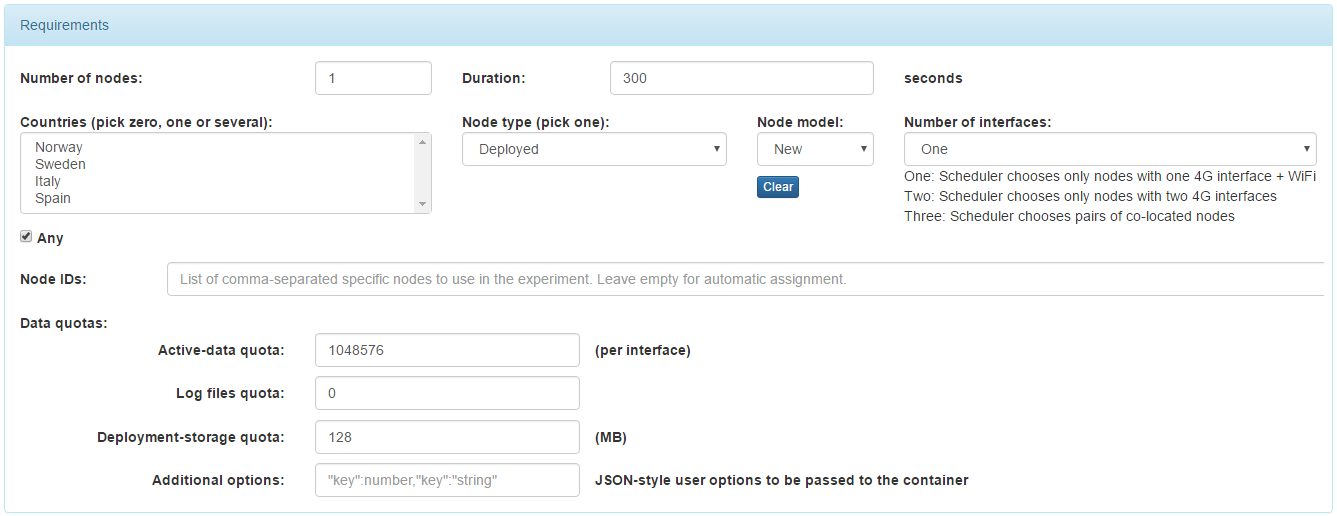
\includegraphics[width=1.0\textwidth]{NewExperimentFilters.png}
	\caption{Filters for node selection.}
	\label{fig:newExperimentFilters}
\end{figure}

\subsection{Experiment scheduling}
\label{subsec:experimentScheduling}

When all the requirements are specified, the user needs to click the ``Submit experiment'' button to submit to the scheduler.
The experiments must respect several restrictions to be successfully scheduled:
\begin{itemize}
	\item The starting time must be at least \SI{10}{\minute} in the future, to allow time for container deployment.
	\item No experiment can be scheduled more than one month in advance.
	\item Periodic experiments must have a period greater than \SI{3600}{\second}.
	The finishing time must also obey the previous rule, that is, the last experiment instance in the recurrence must be scheduled in less than a month from the current time.
	\item No experiment (or instance in a series) can last more than one day.
	In practice, the longest period that an experiment will be awarded is less than \SI{3}{\hour}.
	\item If a list of specific nodes and a starting date are given, the scheduler may be unable to grant the required resources.
%	TODO: Find a way to ease the problem of finding a slot, with perhaps a time-line of resource availability.
\end{itemize}

\subsubsection{Recurrence}
\monroe{}'s scheduler allows to specify experiments that need to be repeated periodically.
In that case, the user has to specify the repetition period ($\ge \SI{3600}{\second}$) and the final stopping date.
The scheduler will treat each repetition as a different experiment and will try to satisfy the requirements for each of them consecutively.
However, the operation is atomic:
Either all the repetitions are scheduled, or none are.

\subsubsection{Checking availability}
If the exact starting time is not relevant, the user can press the ``Check availability'' button.
If the requirements can be satisfied, a message explaining when the experiment might be started will be displayed.
Additionally, it will also inform of the maximum number of nodes that can be used during this period, and the maximum ending time.
With these data, the experimenter may decide to increase the number of nodes that run the experiment, or increase its duration until the time that the scheduler is likely being able to grant.
Figure~\ref{fig:newExperimentCheckAvailability} shows the answer of the scheduler for an availability query.

\begin{figure}[tp]
	\centering
	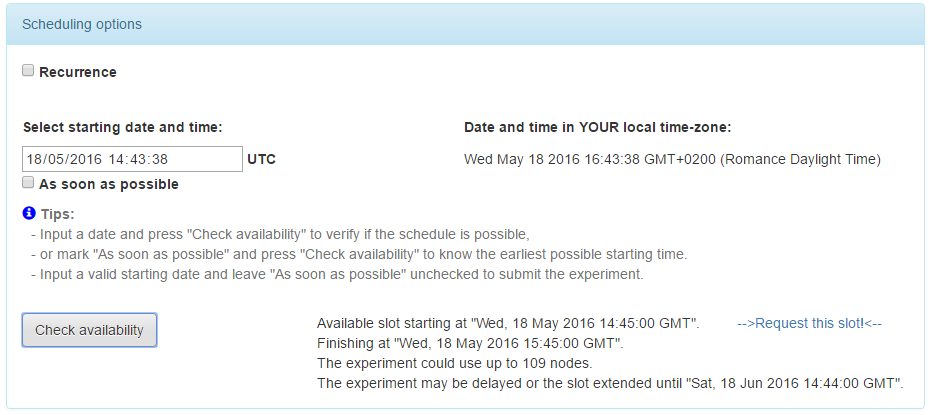
\includegraphics[width=1.0\textwidth]{NewExperimentCheckAvailability.png}
	\caption{The scheduler may supply hints on the scheduling availability, including the earliest starting date that is possible, the end of the availability period for the required resources and the maximum number of nodes, with the specified requirements, that the experiment could reserve. In this example, the experiment can start on ``2017-02-28 16:04:08 UTC'' and can last until ``2017-02-28 16:45:02 UTC.'' The experiment can be scheduled with up to 36 nodes during this period.}
	\label{fig:newExperimentCheckAvailability}
\end{figure}


\subsection{Experiment monitoring}
\label{subsec:experimentMonitoring}

Once an experiment is successfully submitted, the user can check its progress under the ``Status'' tab.
Figure~\ref{fig:ExperimentsSummary} shows an example of a list of experiments.

\begin{figure}[tp]
	\centering
	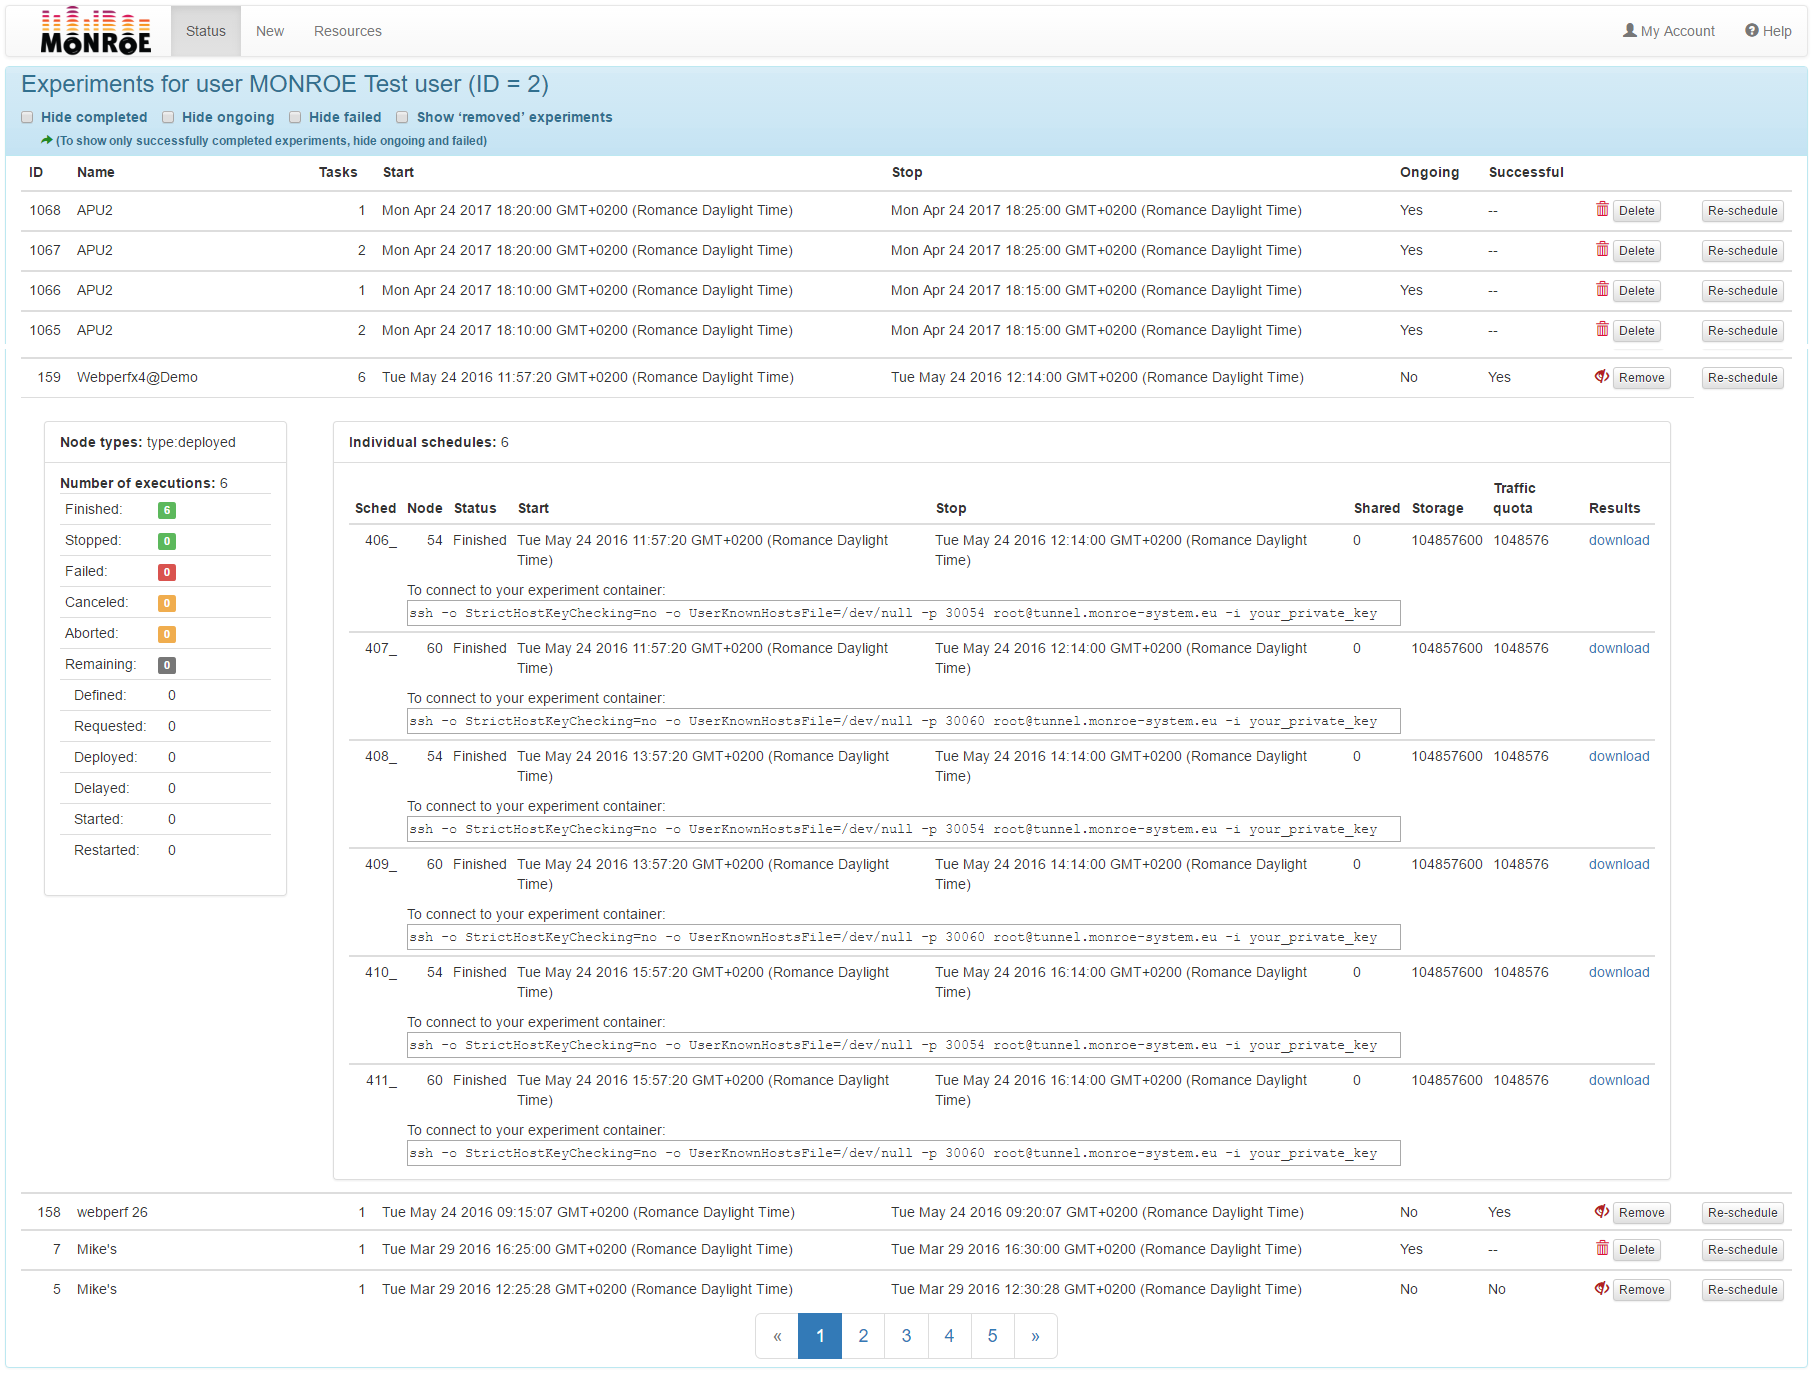
\includegraphics[width=1.0\textwidth]{ExperimentSummary.png}
	\caption{List of user experiments.}
	\label{fig:ExperimentsSummary}
\end{figure}

All the active (i.e., not completed) experiments for the user are shown.
Experiments that have not yet been started can be canceled and deleted.
However, the scheduler will try to stop experiments that have already started, but they will not be deleted from the list.

Clicking on any experiment displays the details for its individual schedules.
There, the number of schedules that are defined but not yet deployed, the ones that are deployed and ready to be started, the ones that are currently running, etc., is summarized.
One line is presented for each individual schedule on each \monroe{} node.
Table~\ref{tab:experimentStates} explains the states in which an individual task may be.

\begin{table}[tp]
	\caption{Experiment states}\label{tab:experimentStates}
	\begin{center}
		\begin{tabular*}{1\textwidth}{p{0.15\textwidth}p{0.8\textwidth}}
			\toprule
			\textbf{STATE} & \textbf{DESCRIPTION} \\ \midrule
			\multicolumn{2}{l}{\textbf{(Ongoing states)}}\\~\\
			\textcolor{blue}{Defined} & The experiment is created in the scheduler. If a task remains in this state past its starting time, the node was probably shut down and the task will not be executed anymore.\\
			\textcolor{blue}{Requested} & The node has requested the container and is deploying it.\\
			\textcolor{blue}{Deployed} & The node has already deployed the container and is waiting for its starting time.\\
			\textcolor{blue}{Delayed} & The scheduling process failed temporarily.\\
			\textcolor{blue}{Started} & The container is being executed in the designated node. The ``download'' link for the task results is already available.\\
			\textcolor{blue}{Restarted} & The node has restarted the experiment after a node failure.\\~\\
			\midrule
			\multicolumn{2}{l}{\textbf{(Final states)}}\\~\\
			\textcolor{green}{Finished} & The task was correctly executed and it finished on its own before consuming the complete time slot.\\
			\textcolor{green}{Stopped} & The task was correctly executed, but it was stopped by the scheduler at the end of the execution slot (correct for tasks designed to remain in execution until the end of their time slot).\\
			\textcolor{red}{Failed} & The task stopped abnormally.\\
			\textcolor{red}{Canceled} & The task was canceled by the user before being started (but other tasks in the experiment were already started).\\
			\textcolor{red}{Aborted} & The task was aborted by the user after being started.\\
			\bottomrule
		\end{tabular*}
	\end{center}
\end {table}

Some experiments may be designed to finish after completion.
For those ones, the correct finishing state is ``Finished.''
If they are stopped by the scheduler, they probably exceeded the execution time foreseen by the experimenter.
However, other experiments may be designed to run continuously for a period of time.
In those cases, the ``Stopped'' state could actually be the correct ending state as intended by the experimenter.

%------------------------------------------------------------%
\FloatBarrier{}
\subsection{Command Line Interface}
\label{subsec:cli}

The \monroe{} scheduler REST API is normally used through the provided WEB interface.
However, experimenters can use it directly to improve task automation.
A complete command-line tool is available at \url{https://github.com/ana-cc/monroe-cli}.%
\footnote{The command-line interface tool has been provided by Ana Custura, from the University of Aberdeen Court, in the context of the MONROE-PREC project.}
The following paragraphs describe how to install and use the tool.

\subsubsection{Installation}

Installation prerequisites:
{\VerbatimFont\begin{verbatim}
sudo apt-get install python3 python3-setuptools python3-cryptography
sudo pip install straight.plugin
\end{verbatim}}

\noindent From the directory that contains the tool sources:
{\VerbatimFont\begin{verbatim}
python3 setup.py develop
\end{verbatim}}

\noindent The user certificate can be imported with:
{\VerbatimFont\begin{verbatim}
$ monroe setup --cert MyCert.p12
Enter passphrase:
Your certificate files were stored in ~/.monroe
\end{verbatim}}
This feature depends on a recent version of OpenSSH.
Alternatively, the cert/key files can be extracted manually and placed under \identifier{$\sim$/.monroe/}  with the names \identifier{mnrCrt.pem} and \identifier{mnrKey.pem}.

\subsubsection{Usage}

The tool has integrated help:
{\VerbatimFont\begin{verbatim}
$ monroe -h
 usage: monroe [-h] Command ...
 
 Monroe Cli
 
 optional arguments:
 -h, --help   show this help message and exit
 
 Experiment:
 The following commands can be used to create and submit experiments
 
 Command      Description
 create     Creates an experiment
 whoami     Displays MONROE user details
 quota      Displays MONROE quota details
 experiments
 Display recent experiments
 setup      Specifies MONROE user certificate to use for accessing the
 scheduler
 delete     Deletes an experiment
 results    Downloads the results for an experiment
\end{verbatim}}

\noindent Correct installation of the tool can be tested trying to retrieve the user identification:
{\VerbatimFont\begin{verbatim}
$ monroe whoami
Authentication ID: 2, Name: MONROE Test user, Storage Quota remaining: 49597346816 bytes
\end{verbatim}}

\noindent User quotas can be easily retrieved:
{\VerbatimFont\begin{verbatim}
$ monroe quota
2017-05-05 : Remaining time is 138888.00 hours.
2017-05-05 : Remaining storage quota is 46.00 GB.
2017-05-05 : Remaining data quota is 46.00 GB.
\end{verbatim}}

\noindent The tool allows retrieving the list of recent experiments:
{\VerbatimFont\begin{verbatim}
$ monroe experiments
Experiment ID: 6798 Name: mike test on new nodes Script: steven76/headless Summary: {u'aborted': 1}
Experiment ID: 6799 Name: mike test on new nodes Script: steven76/headless Summary: {u'aborted': 1}
Experiment ID: 6800 Name: mike test on new nodes Script: steven76/headless Summary: {u'aborted': 1}
\end{verbatim}}

\noindent The results of an experiment can also be automatically retrieved:
{\VerbatimFont\begin{verbatim}
$ monroe results --exp 6479
\end{verbatim}}
\noindent This command downloads the experiment results into \identifier{6479/sched\_id}, for all the task IDs associated to that experiment.

For experiment creation, the tool supports defining SSH access to the container (in testing nodes), additional options and recurrence.
Finally, the tool can be used as a library:
{\VerbatimFont\begin{verbatim}
from monroe.core import *
\end{verbatim}}


%------------------------------------------------------------%
%------------------------------------------------------------%
%------------------------------------------------------------%

\section{Retrieval of metadata and experiment results}
\label{sec:resultRetrieval}

\monroe{} repositories contain two types of data: \monroe{} metadata itself and the results of user experiments.

%------------------------------------------------------------%
\subsection{User experiment results}

Any files written during the experiment to the \identifier{/monroe/results} directory will be synchronized to the experiment repository.
This operation happens continuously during experiment execution and then upon its finalization.
Therefore, it is advisable that only final files ready to be transferred are copied (indeed, mv'ed) to that location to avoid the system to sync temporary files and consume your quota or produce invalid results.
This recommendation means that files in the results folder should not be updated; experimenters are encouraged to copy intermediate result files as soon as they are ready so they can retrieve partial results if the experiment fails in the middle of its execution.

The result files can be accessed through the user interface:
For experiments that have already been started, the interface presents a link under the column ``Results'' that redirects the user to the HTTP folder (Figure~\ref{fig:ResultsRetrieval}) that contains the files already synchronized from the node where the experiment runs to the repository.
In this way, the experimenter can retrieve result files even for partial experiments that fail or are canceled.

\begin{figure}[tp]
	\centering
	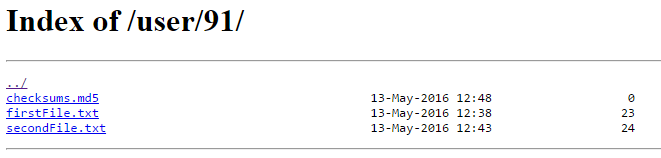
\includegraphics[width=0.7\textwidth]{ResultsRetrieval.png}
	\caption{Folder containing the results of an individual schedule, transferred to \monroe{}'s servers.}
	\label{fig:ResultsRetrieval}
	\end{figure}

In addition, the experiment may use any network functionalities to communicate with outside servers as needed (e.g., \identifier{scp} some files to an external server).
In order to improve safety, private keys should be restricted to the experiments and discarded after a reasonable time.
Additionally, instead of saving your keys in the container itself, you may want to pass them as additional options during experiment scheduling.
The values will be available during container execution as a JSON file at \identifier{/monroe/config}.
Notice that this file is created by the node scheduler.
The same effect is achievable when the containers are run manually in user development nodes adding the \identifier{-v} option to the command line.
To map both a locally created config file and the results folder of the container to a node folder, in development nodes without a scheduler, the following command line fragment may be used:\footnote{Thanks to Eneko Atxutegi Narbona and Jonas Karlsson for pointing this out.}
\begin{verbatim}
-v /monroe/results:/monroe/results -v /monroe/config:/monroe/config:ro
\end{verbatim}

%------------------------------------------------------------%
\subsection{\monroe{} metadata}

\monroe{} metadata can be freely accessed by two means.
First, a CSV dump of all database tables is generated daily.
The files can be accessed at the following URL (a valid user certificate is needed): \url{https://www.monroe-system.eu/user/dailyDumps/}.
The dump files should be available every day after 12:00 CET (24-hour format).
Each file covers the period [00:00, 00:00) GMT.

Our servers run on CET time, but metadata timestamps use GMT.
Therefore, to cover ``a day'' of metadata using, e.g., the local time in Norway, two CSV files need to be combined.
During Winter time, the needed metadata is in the period [day$_0$:01:00, day$_1$:01:00).
During Summer time, the needed metadata is in the period [day$_0$:02:00, day$_1$:02:00).

Alternatively, metadata can be accessed directly in a replica of \monroe{}'s Cassandra database, which is updated daily approximately at noon with the data from the previous (GMT) day.
Access credentials for this server will be provided as requested.
\monroe{} repositories include several examples on how to access the database.


%------------------------------------------------------------%
%------------------------------------------------------------%
%------------------------------------------------------------%

\section{Run-time considerations for experimenters}
\label{sec:experimentRuntime}

This section discusses several considerations that experimenters must take into account when designing and running their experiments on the \monroe{} platform.

%------------------------------------------------------------%
\subsection{Node identification}
\label{subsec:nodeIdentification}

An experiment can identify the node it is running on by reading the contents of the \identifier{/etc/nodeid} file:
{\VerbatimFont
\begin{verbatim}
cat /etc/nodeid
54
\end{verbatim}}

%------------------------------------------------------------%
\subsection{Communication during the experiment}
\label{subsec:communicationDuringExperiment}

During execution, the experiment is free to establish any network communications through the available interfaces.
The user can choose to bind explicitly from each command or application to a specific interface, or they may define default routes during the experiment:
{\VerbatimFont\begin{verbatim}
	route add default gw 172.16.0.1 eth0
\end{verbatim}}

%------------------------------------------------------------%
\subsection{Interface naming and default route}
\label{subsec:interfaceNaming}

To offer a consistent view of the platform resources, whereas allowing flexibility for future changes in the platform configuration, the following naming scheme is used for each of the interfaces available for the experiments:
\begin{enumerate*}
	\item [\textbf{op0}:] First mobile interface.
	\item [\textbf{op1}:] Second mobile interface.
	\item [\textbf{op2}:] Only for old nodes, third mobile interface.
	\item [\textbf{eth0}:] Ethernet (wired) network connection, when available.
\end{enumerate*}
The platform guarantees that a given op$_i$ corresponds to the same operator during experiment execution.
However, \emph{the assignment may change} between nodes in the same country or even between successive executions in the same node.
Therefore, \emph{experiments must check the metadata stream} to select the correct interface associated to the desired operator.

Under some circumstances, the mobile devices used in the \monroe{} nodes may loose connectivity, reset themselves or undergo any other process that makes them temporarily unavailable for the experiments.
To identify and tackle with these situations, experimenters are encouraged to build ``robust'' experiments subscribing to the corresponding metadata streams.

If the experimenter writes their own code:
\begin{enumerate*}
	\item Subscribe to the metadata broadcast.
	\item Wait for a \identifier{MODEM.*.UPDATE} message for the modem(s)/operators of interest.
	\item Once this information is obtained, use the desired interface and store the results with the corresponding ICCID or operator name.
	\item Should the interface disappear (\identifier{ENODEV} error, ``no such device''), start over at 2.
\end{enumerate*}
	
When using an external tool that does not handle \identifier{ENODEV} (e.g., ``fping''), replace step 4 by:
\begin{itemize*}
	\item Monitor the metadata for a \identifier{MODEM.*.CONNECTIVITY} message indicating that connectivity was lost, or monitor the interface list to check if the device disappears. Upon either event, start over at 2.
\end{itemize*}
	
Experimenters should take notice that an interface may not only go down, but it may actually disappear from the list of available interfaces (e.g., if the modem has to be restarted).
Even if it reappears soon after, any existing network connections on the old interface will fail with \identifier{ENODEV}. 
	
It is also possible to skip steps 1 and 2 when reconnecting to an interface after a failure, as the interface name corresponding to the desired operator is already known.
It is still necessary to keep retrying to connect to the interface, until it comes up.

%------------------------------------------------------------%
\subsection{Interface binding}
\label{subsec:binding}

Experiments running in \monroe{} nodes have access to several network interfaces.
By default, that is, if the experiment does not take any special configuration actions, the default route will be configured to one of the mobile broadband interfaces, if available.
However, experimenters have the possibility of explicitly binding external tools or their programs to specific interfaces.
Several options are available to bind an experiment to an interface.

\begin{enumerate*}
	\item Most standard tools can be instructed to use an specific interface:
	{	\VerbatimFont
		\begin{verbatim}
		ping -I op0 host_name
		tcpdump --I op0 target
		wget --bind-address ...
		curl --interface ...
		\end{verbatim}
	}
	
	\item Explicit binding in the source code.
	\begin{itemize*}
		\item In C:
		{
			\VerbatimFont
			\begin{verbatim}
			snprintf(ifr.ifr_name, sizeof(ifr.ifr_name), "op0");
			setsockopt(s, SOL_SOCKET, SO_BINDTODEVICE, (void *)&ifr, sizeof(ifr))
			localaddr.sin_addr.s_addr = inet_addr("192.168.1.100");
			bind(sockfd, (struct sockaddr *)&localaddr, sizeof(localaddr));
			\end{verbatim}
		}
		\item In Python:
		{
			\VerbatimFont
			\begin{verbatim}
			s = socket.socket()
			s.bind('192.168.1.152', 0))
			\end{verbatim}
		}
	\end{itemize*}
	
	\item Library overloading the \identifier{bind()} and \identifier{connect()} functions through \identifier{LD\_PRELOAD}:
	
	\url{http://www.ryde.net/code/bind.c.txt}
	
	\item Changing the default route:
	{
		\VerbatimFont
		\begin{verbatim}
		route del default gw ...; route add ...
		\end{verbatim}
	}
\end{enumerate*}


%------------------------------------------------------------%
\subsection{Metadata at run-time}
\label{subsec:metadataRunTime}

\monroe{} nodes retrieve constantly some metadata information concerning their own state and the network conditions.
This information is continuously uploaded to the \monroe{} servers and stored in a database.
One of the main goals of the \monroe{} project is to make all that information freely accessible.
Therefore, experimenters may perform an off-line correlations of events in their experiment with the information in the \monroe{} database.

\monroe{} experimenters can also access all the metadata information at run-time from their experiments to achieve easy correlation of events or modify the behavior of the experiment during its execution. For example:
\begin{itemize*}
	\item Experiments that depend on external factors (location):
	\begin{itemize*}
		\item Round trip time vs. location.
		\item Proactive HTTP caching according to location.
		\item Round trip time vs. base station.
		\item Round trip time vs. signal strength.
		\item Route selection according to current conditions.
	\end{itemize*}
	\item Experiment validation:
	\begin{itemize*}
		\item Verify that node temperature is/was within limits.
		\item Verify that system load is/was below threshold.
	\end{itemize*}	
\end{itemize*}

The metadata is broadcast locally using ZeroMQ.
The following excerpt in Python shows how an application can subscribe to the metadata stream:
{\VerbatimFont
\begin{verbatim}
import zmq

context = zmq.Context()
socket = context.socket(zmq.SUB)
socket.connect ("tcp://172.17.0.1:5556")

# An empty string subscribes to everything:
topicfilter = ''   # E.g., use 'MONROE.META.DEVICE.GPS' for GPS-only metadata
socket.setsockopt(zmq.SUBSCRIBE, topicfilter)

while True:
  string = socket.recv()
  print string
\end{verbatim}
}

%------------------------------------------------------------%
\subsubsection{Example: Correlate experiment results with metadata at run-time}

The following example shows how to create an application that executes a ping to an external machine and saves the results alongside the node location:

\begin{itemize*}
	\item Pipe the ping command through a ``ping formatter.''
	\item The ``ping'' formatter subscribes to a zmq socket and topic:
	\begin{itemize*}
		\item Socket : 'tcp://172.17.0.1:5556'
		\item Topic : 'MONROE.META.DEVICE.GPS' 
	\end{itemize*}
	\item Cache the GPS position received. 
	\item Wait for output from the ping command (stdin).
	\item Store experiment information including the GPS position:
	\begin{itemize*}
		\item Use the ``library'' \identifier{monroe\_exporter} (python only).
		\item Call the \identifier{monroe\_exporter} script via the command line.
	\end{itemize*}
\end{itemize*}

Below is the corresponding source code:
{\VerbatimFont
\begin{verbatim}
socket.connect('tcp://localhost:5557')
socket.setsockopt(zmq.SUBSCRIBE, 'MONROE.META.DEVICE.GPS')
LAST_GPS_FIX = None

monroe_exporter.initalize('MONROE.EXP.PING', 1, 5.0)

'''fork and wait for for gps messages'''
while True:
  (topic, msgdata) = socket.recv_multipart()
  LAST_GPS_FIX = json.loads(msgdata)

'''main process waits for ping experiment output '''
while line:
  exp_result = r.match(line).groupdict()
  msg = {
    'InterfaceName': interface,
    'Bytes': int(exp_result['bytes']),
    'Host': exp_result['host'],
    'Rtt': float(exp_result['rtt']),
    'SequenceNumber': int(exp_result['seq']),
    'TimeStamp': float(exp_result['ts'])
  }
  if LAST_GPS_FIX != None:
    msg.update(
      {
        'GPSTimeStamp': LAST_GPS_FIX['TimeStamp'],
        'Latitude': LAST_GPS_FIX['Latitude'],
        'Longitude': LAST_GPS_FIX['Longitude'],
        'Altitude': LAST_GPS_FIX['Altitude'],
        'NumberofSatellites': LAST_GPS_FIX['NumberofSatellites']
          })

  monroe_exporter.save_output(msg)
  line = sys.stdin.readline()
\end{verbatim}
}
 
%------------------------------------------------------------%
\subsubsection{Metadata information}

Currently, the collected metadata includes:
\begin{itemize*}
	\item Node GPS.
	\item Node sensors (CPU temp) and probes (load, memory usage).
	\item Modem status and events.
	\item Continuous and scheduled internal experiments:
	\begin{itemize*}
		\item RTT (through ping).
		\item Bandwidth (through HTTP download).
	\end{itemize*}
\end{itemize*}

The following and some examples of the information received in the metadata stream:

\begin{itemize}
	\item RTT experiment:\\
	\texttt{\footnotesize\{"\textbf{DataId}": "MONROE.EXP.PING", "\textbf{Bytes}": 84, "\textbf{NodeId}": "54", \\
		"\textbf{SequenceNumber}": 301, "\textbf{DataVersion}": 1, "\textbf{Timestamp}": 1465805479.747943, \\
		"\textbf{Rtt}": 71.2, "\textbf{Host}": "8.8.8.8", "\textbf{Operator}": "Orange", \\
		"\textbf{Iccid}": "8934014251541036013", "\textbf{Guid}": \\ "sha256:a9f9fb2c04bba3782ef2624e118faa18f16b08c826155cae5e1ea7e1d88832b5.0.54.3791"\}}

	\item Sensors, where each message may contain information about a different set of measurements:\\
	\texttt{\footnotesize\{"\textbf{DataId}": "MONROE.META.NODE.SENSOR", "\textbf{softirq}": "205270", "\textbf{SequenceNumber}": 48581,\\
		"\textbf{DataVersion}": 1, "b": "1059270", "b": "4885494", "\textbf{guest}": "0", "\textbf{NodeId}": "54", \\
		"\textbf{idle}": "42657942", "\textbf{user}": "10480984", "\textbf{irq}": "0", "\textbf{steal}": "0", \\
		"\textbf{Timestamp}": 1465786966.123456, "\textbf{nice}": "3063"\}}\\~\\
	\texttt{\footnotesize\{"\textbf{DataId}": "MONROE.META.NODE.SENSOR", "\textbf{SequenceNumber}": 48567, "\textbf{DataVersion}": 1,\\
		"\textbf{Timestamp}": 1465786961.123456, "\textbf{percent}": "65.98", "\textbf{NodeId}": "54", "\textbf{current}": "302234", \\
		"\textbf{start}": "1465484726", "\textbf{total}": "5246545.72", "\textbf{id}": "39"\}}\\~\\
	\texttt{\footnotesize\{"\textbf{DataId}": "MONROE.META.NODE.SENSOR", "\textbf{SequenceNumber}": 48460, "\textbf{DataVersion}": 1,\\
		"\textbf{Timestamp}": 1465786926.123456, "\textbf{apps}": "3632746496", "\textbf{NodeId}": "54", "\textbf{free}": "483119104", \\
		"\textbf{swap}": "0"\}}
	
	\item Modem events:\\
	\texttt{\footnotesize\{"\textbf{DataId}": "MONROE.META.DEVICE.MODEM", "\textbf{InterfaceName}": "usb2", "\textbf{CID}": 72209509,\\
		"\textbf{DeviceState}": 3, "\textbf{SequenceNumber}": 33548, "\textbf{DataVersion}": 1, \\
		"\textbf{Timestamp}": 1465803136.123456, \\
		"\textbf{NWMCCMNC}": 21404, "\textbf{Band}": 3, "\textbf{RSSI}": -80, "\textbf{IPAddress}": "10.33.101.173", \\
		"\textbf{IMSIMCCMNC}": 21404, "\textbf{DeviceMode}": 5, "\textbf{NodeId}": "54", "\textbf{IMEI}": "864154023645179", \\
		"\textbf{RSRQ}": -8, "\textbf{RSRP}": -85, "\textbf{LAC}": 28014, "\textbf{Frequency}": 1800, \\
		"\textbf{InternalIPAddress}": "192.168.0.153", "\textbf{Operator}": "YOIGO", \\
		"\textbf{ICCID}": "8934041514050774002", "\textbf{IMSI}": "214040113950108"\}}
	
	\item GPS:\\
	\texttt{\footnotesize\{"\textbf{DataId}": "MONROE.META.DEVICE.GPS", "\textbf{SequenceNumber}": 34164, "\textbf{DataVersion}": 1, \\
		"\textbf{Timestamp}": 1465805718.123456, "\textbf{Altitude}": -1455.900024, "\textbf{NodeId}": "63", \\
		"\textbf{Longitude}": -3.777019, "\textbf{NMEA}":\\ "\$GPGGA,081518.0,4020.002011,N,00346.621107,W,1,02,500.0,-1455.9,M,53.0,M,,*5D\textbackslash{}r\textbackslash{}n",\\
		"\textbf{SatelliteCount}": 2, "\textbf{Latitude}": 40.333366\}}
	
\end{itemize}

%------------------------------------------------------------%
\subsubsection{Metadata format}
Metadata and internal experiment results follow a JSON structure, as detailed in \url{https://github.com/MONROE-PROJECT/Experiments/wiki}~:
\begin{itemize*}
	\item All Metadata messages have a topic according to Table~\ref{tab:metadataTopics}. Appendix~\ref{app:metadataFields} gives the complete description of the meaning of all the metadata fields.
	\item All metadata topics are prefixed with ``MONROE.META.''
	\item All internal experiments are prefixed with ``MONROE.EXP.''
	\item Experiments receive metadata messages only for topics to which they subscribe.
	\item An empty string ("") subscribes to all topics.
\end{itemize*}

\begin{table}[tp]
	\caption{Metadata topics.}\label{tab:metadataTopics}
	\begin{center}
	\begin{tabular}{ll}
		\toprule
		\textbf{TOPIC} & \textbf{DESCRIPTION} \\
		\midrule
		*.DEVICE.MODEM.iccid.UPDATE	& \\
		*.DEVICE.MODEM.iccid.MODE & \\
		*.DEVICE.MODEM.iccid.SIGNAL	& \\
		*.DEVICE.MODEM.iccid.LTEBAND	& \\
		*.DEVICE.MODEM.iccid.ISPNAME	& \\
		*.DEVICE.MODEM.iccid.IPADDR	& \\
		*.DEVICE.MODEM.iccid.LOCCHANGE	& \\
		*.DEVICE.MODEM.iccid.NWMCCMNCCHANGE	& \\
		*.DEVICE.GPS	& \\
		*.NODE.SENSOR.sensor\_name & Temp sensor, running experiments, quotas, \ldots \\
		*.NODE.EVENT & Power up events, etc, \ldots \\
		\bottomrule
	\end{tabular}
	\end{center}
\end{table}

%------------------------------------------------------------%
\subsection{Tstat at run-time}
\label{subsec:tsattRunTime}
The Tstat (\url{http://www.tstat.polito.it/}) \textbf{runs} on all nodes in the mPlane container as one of the basic MONROE containers. The Tstat is a passive probe able to provide several insight on the traffic patterns at both the network and the transport levels. The Tstat generates two different types of logs. 

\subsubsection{Tstat Round Robin Database}

\begin{figure}[h]
	\centering
	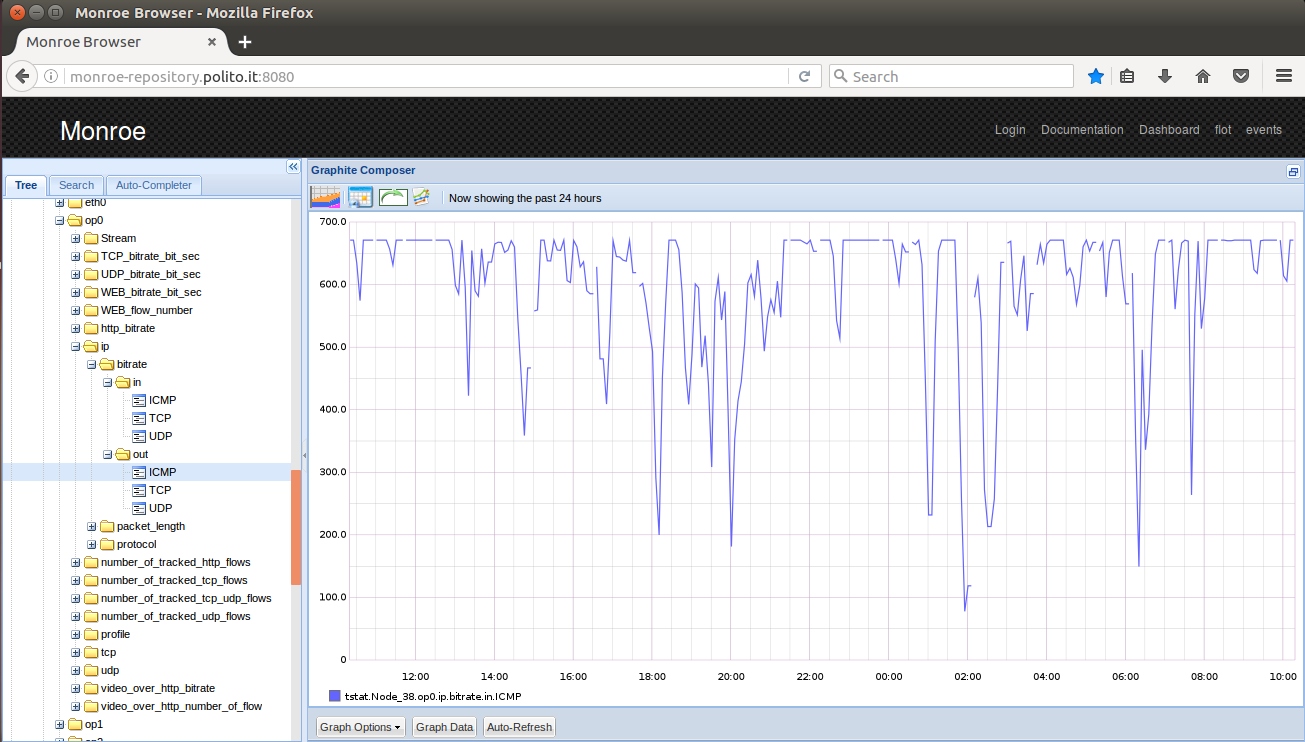
\includegraphics[width=1\textwidth]{TstatRRDGUI.png}
	\caption{Graphite GUI of the Tstat RRD logs.}
	\label{fig:TstatRRDGUI}
\end{figure}

The RRD (Round Robin Database) logs is an average of samples of each packet in 5 minutes, it imposes at least 5 minutes delay to visualize RRDs. The detail description of the RRD logs is available on Tstat documentation(\url{http://tstat.polito.it/HOWTO.shtml#RRD}). RRD are available via the (\url{http://monroe-repository.polito.it:8080/}) and the Graphite GUI provides some tool to present RRD logs and save the interested plots. Fig.~\ref{fig:TstatRRDGUI} shows the bit rate of the ICMP packet for the node \#38 on interface \textit{op0} over the last 24 hours. 
There is possibility to create a dashboard to monitor the experiments and interfaces' status. Fig.~\ref{fig:TStatGraphitedashboard} illustrates an example of saved dashboard to monitor the volume of traffic on one node. 

\begin{figure}[h]
	\centering
	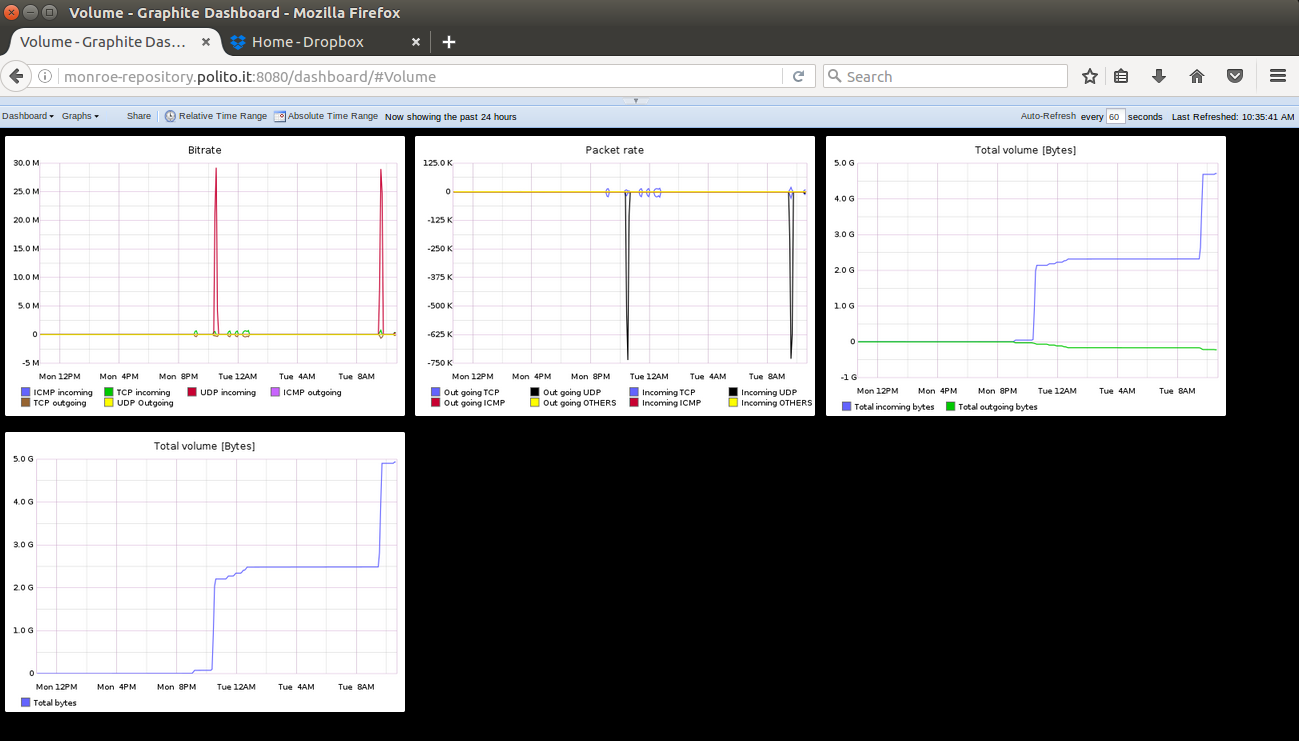
\includegraphics[width=1.0\textwidth]{TStatGraphitedashboard.png}
	\caption{An example of dashboard on Tstat RRD GUI.}
	\label{fig:TStatGraphitedashboard}
\end{figure}


\subsubsection{Tstat logs}
Tstat generates detailed flow level logs for TCP, UDP, and HTTP flows. These are text file with more than 100 metrics, containing information about the client and server addresses, network and application level metrics, and DNS queries. The description of the metrics presents (\url{http://tstat.polito.it/measure.shtml#LOG}).
In MONROE, the Tstat configure to generate 4 different logs as following:

\begin{table}[h]
	\caption{Tstat log types.}\label{tab:Tstatlogs}
	\begin{center}
	\begin{tabular}{ll}
		\toprule
		\textbf{TYPE} & \textbf{DESCRIPTION} \\
		\midrule
		log\_tcp\_complete & Every TCP connection that has been tracked \\
		log\_tcp\_nocomplete	& All the connections for which the three way handshake is not properly seen \\
		log\_udp\_complete & Every tracked UDP flow pair \\
		log\_http\_complete & Information from every HTTP request and response \\
			\bottomrule
	\end{tabular}
	\end{center}
\end{table}
    
Logs are available in two ways, 
\begin{itemize}
\item[1.] Real time access on the node, logs for the last three generated are shared with MONROE experimenters on the "/monroe/tstat", it helps the MONROE users to use passive traces collected by Tstat during their experiment. The three logs can cover at most the last three hours.
\item[2.] On demand, all logs are imported into MONROE database for all node. The schema of the tables are available on github (\url{https://github.com/MONROE-PROJECT/Database/blob/master/db_schema.cql}). Three columns, (NodeId,Iccid,DataId) added to each table bring the possibility to join with metadata and collected data. 
\end{itemize}

It is recommended to check the description of the logs on (\url{http://tstat.polito.it/measure.shtml#LOG}).  Tables~\ref{tab:TStattcp},~\ref{tab:TStattcprtt} and~\ref{tab:TStathttp}  present the table describing of some interesting metrics in tcp and http logs.
\begin{table}[tp]
	\caption{Core TCP Set.}\label{tab:TStattcp}
	\TableFont{
		\begin{center}
			\rowcolors{1}{LightYellow}{LightYellow}
			\begin{tabular*}{1\textwidth}{|l|l|l|l|p{0.6\textwidth}}
				\toprule
				\cellcolor{BrightYellow}\textbf{C2S}		& \cellcolor{BrightYellow}\textbf{S2C} & \cellcolor{BrightYellow}\textbf{Short description} & \cellcolor{BrightYellow}\textbf{Unit}	& \cellcolor{BrightYellow}\textbf{Long description}\\ \midrule
				1	& 15	& Client/Server IP addr		& --	& IP addresses of the client/server\\ \hline
				2	& 16	& Client/Server TCP port	& --	& TCP port addresses for the client/server\\ \hline
				3	& 17	& packets					& --	& total number of packets observed from the client/server\\
				4	& 18	& RST sent					& 0/1	& 0 = no RST segment has been sent by the client/server\\
				5	& 19	& ACK sent					& --	& number of segments with the ACK field set to 1\\
				6	& 20	& PURE ACK sent				& --	& number of segments with ACK field set to 1 and no data\\ \hline
				7	& 21	& unique bytes				& \si{\byte}	& number of bytes sent in the payload\\ \hline
				8	& 22	& data pkts					& --	& number of segments with payload\\ \hline
				9	& 23	& data bytes				& \si{\byte}	& number of bytes transmitted in the payload, including retransmissions\\ \hline
				10	& 24	& rexmit pkts				& --	& number of retransmitted segments\\ \hline
				11	& 25	& rexmit bytes				& \si{\byte}	& number of retransmitted bytes\\ \hline
				12	& 26	& out seq pkts				& --	& number of segments observed out of sequence\\ \hline
				13	& 27	& SYN count					& --	& number of SYN segments observed (including rtx)\\ \hline
				14	& 28	& FIN count					& --	& number of FIN segments observed (including rtx)\\ \hline
				\rowcolor{PalePink}\multicolumn{2}{l|}{29}	& First time abs	& \si{\milli\second}	& Flow first packet absolute time (epoch)\\ \hline
				\rowcolor{PalePink}\multicolumn{2}{l|}{30}	& Last time abs		& \si{\milli\second}	& Flow last segment absolute time (epoch)\\ \hline
				\rowcolor{PalePink}\multicolumn{2}{l|}{31}	& Completion time	& \si{\milli\second}	& Flow duration since first packet to last packet\\ \hline
				\rowcolor{PalePink}\multicolumn{2}{l|}{32}	& C first payload	& \si{\milli\second}	& Client first segment with payload since the first flow segment\\
				\rowcolor{PalePink}\multicolumn{2}{l|}{33}	& S first payload	& \si{\milli\second}	& Server first segment with payload since the first flow segment\\
				\rowcolor{PalePink}\multicolumn{2}{l|}{34}	& C last payload	& \si{\milli\second}	& Client last segment with payload since the first flow segment\\
				\rowcolor{PalePink}\multicolumn{2}{l|}{35}	& S last payload	& \si{\milli\second}	& Server last segment with payload since the first flow segment\\ \hline
				\rowcolor{PalePink}\multicolumn{2}{l|}{36}	& C first ack		& \si{\milli\second}	& Client first ACK segment (without SYN) since the first flow segment\\ \hline
				\rowcolor{PalePink}\multicolumn{2}{l|}{37}	& S first ack		& \si{\milli\second}	& Server first ACK segment (without SYN) since the first flow segment\\ \hline
				\rowcolor{LightGreen}\multicolumn{2}{l|}{38}	& C internal		& 0/1					& 1 = client has internal IP, 0 = client has external IP\\ \hline
				\rowcolor{LightGreen}\multicolumn{2}{l|}{39}	& S internal		& 0/1					& 1 = server has internal IP, 0 = server has external IP\\ \hline
				\rowcolor{LightGreen}\multicolumn{2}{l|}{40}	& C anonymized		& 0/1					& 1 = client IP is CryptoPAn anonymized\\ \hline
				\rowcolor{LightGreen}\multicolumn{2}{l|}{41}	& S anonymized		& 0/1					& 1 = server IP is CryptoPAn anonymized\\ \hline
				\multicolumn{2}{l|}{42}	& Connection type	& --				& Bitmap stating the connection type as identified by TCPL7 inspection engine (see protocol.h)\\ \hline
				\multicolumn{2}{l|}{43}	& P2P type			& --				& Type of P2P protocol, as identified by the IPP2P engine (see ipp2p\_tstat.h)\\ \hline
				\multicolumn{2}{l|}{44}	& HTTP type			& --				& For HTTP flows, the identified Web2.0 content (see the http\_content enum in struct.h)\\
				\bottomrule
			\end{tabular*}
		\end{center}
	}
	\end {table}


\begin{table}[tp]
	%\setlength\arrayrulewidth{0.75pt}
	\caption{TCP End to End Set.}\label{tab:TStattcprtt}
	\TableFont{
		\begin{center}
			\rowcolors{1}{LightYellow}{LightYellow}
			\begin{tabular*}{1\textwidth}{|l|l|l|l|p{0.65\textwidth}}
				\toprule
				\cellcolor{BrightYellow}\textbf{C2S}		& \cellcolor{BrightYellow}\textbf{S2C} & \cellcolor{BrightYellow}\textbf{Short description} & \cellcolor{BrightYellow}\textbf{Unit}	& \cellcolor{BrightYellow}\textbf{Long description}\\ \midrule
				45	& 52	& Average rtt	& \si{\milli\second}	& Average RTT computed measuring the time elapsed between the data segment and the corresponding ACK\\ \hline
				46	& 53	& rtt min		& \si{\milli\second}	& Minimum RTT observed during connection lifetime\\ \hline
				47	& 54	& rtt max		& \si{\milli\second}	& Maximum RTT observed during connection lifetime\\ \hline
				48	& 55	& Stdev rtt		& \si{\milli\second}	& Standard deviation of the RTT\\ \hline
				49	& 56	& rtt count		& --					& Number of valid RTT observation\\ \hline
				50	& 57	& ttl\_min		& --					& Minimum Time To Live\\
				51	& 58	& ttl\_max		& --					& Maximum Time To Live\\
				\bottomrule
			\end{tabular*}
		\end{center}
	}
	\end {table}


\begin{table}[tp]
	\caption{Core HTTP Set.}\label{tab:TStathttp}
	\TableFont{
	\begin{center}
		\rowcolors{1}{LightYellow}{LightYellow}
		\begin{tabular*}{1\textwidth}{|l|l|l|l|p{0.65\textwidth}}
			\toprule
			\cellcolor{PalePink}\textbf{C2S}		& \cellcolor{LightGreen}\textbf{S2C} & \cellcolor{BrightYellow}\textbf{Short description} & \cellcolor{BrightYellow}\textbf{Unit}	& \cellcolor{BrightYellow}\textbf{Long description}\\ \midrule
			\cellcolor{PalePink}1					& \cellcolor{LightGreen}1			& Client IP addr	& --	& IP addresses of the client (sending the request/receiving the response) \\ \hline
			\cellcolor{PalePink}2					& \cellcolor{LightGreen}2			& Client TCP port	& --	& TCP port addresses for the client \\ \hline
			\cellcolor{PalePink}3					& \cellcolor{LightGreen}3			& Server IP addr	& --	& IP addresses of the server (receiving the request/sending the response) \\ \hline
			\cellcolor{PalePink}4					& \cellcolor{LightGreen}4			& Server TCP port	& --	& TCP port addresses for the server \\ \hline
			\cellcolor{PalePink}5					& \cellcolor{LightGreen}5			& Segment time abs	& \si{s}& Absolute time [s] (epoch) of the request/response \\ \hline
			\cellcolor{PalePink}6					& 									& Request method	& --	& Request method (GET/POST/HEAD) [*] \\ \hline
			\cellcolor{PalePink}7					& 									& Hostname			& --	& Value fo the ``Host:'' HTTP request field \\ \hline
			\cellcolor{PalePink}8					& 									& FQDN				& --	& DN-Hunter cached DNS name [\^{}] \\ \hline
			\cellcolor{PalePink}9					& 									& URL Path			& --	& URL request path \\ \hline
			\cellcolor{PalePink}10					& 									& Referer			& --	& Value of the ``Referer:'' HTTP request field \\ \hline
			\cellcolor{PalePink}11					& 									& User agent		& --	& Value of the ``User-Agent:'' HTTP request field \\ \hline
			\cellcolor{PalePink}12					& 									& Cookie			& --	& Value of the ``Cookie:'' HTTP request field \\ \hline
			\cellcolor{PalePink}13					& 									& Do Not Track		& --	& Value of the ``DNT:'' HTTP request field \\ \hline
													& \cellcolor{LightGreen}6			& Response string	& --	& Response identifier (always ``HTTP'') [*] \\ \hline
													& \cellcolor{LightGreen}7			& Response code		& --	& HTTP response code (2xx/3xx/4xx/5xx) \\ \hline
													& \cellcolor{LightGreen}8			& Content len		& \si{\byte}	& Value of the ``Content-Length:'' HTTP response field \\ \hline
													& \cellcolor{LightGreen}9			& Content type		& --	& Value of the ``Content-Type:'' HTTP response field \\ \hline
													& \cellcolor{LightGreen}10			& Server			& --	& Value of the ``Server:'' HTTP response field \\ \hline
													& \cellcolor{LightGreen}11			& Range				& --	& Value of the ``Content-Range:'' HTTP response field for partial content (Code 206) \\ \hline
													& \cellcolor{LightGreen}12			& Location			& --	& Value of the ``Location:'' HTTP response field for redirected content (Code 302) \\ \hline
													& \cellcolor{LightGreen}13			& Set Cookie		& --	& Value of the ``Set-Cookie:'' HTTP response field \\
			\bottomrule
		\end{tabular*}
	\end{center}
	}
\end {table}

%------------------------------------------------------------%
\subsection{Access to user-owned development nodes}

This section refers to development nodes owned by external users under the dispositions of their specific \monroe{} agreement.
Two options are possible for the management of those nodes:
\begin{enumerate*}
	\item The nodes join the pool of \monroe{} nodes.
	Experiments are scheduled through the \monroe{} scheduler and users, including the node owners, do not have direct SSH access to them.
	The metadata produced by these nodes will join the rest of the \monroe{} databases.
	\item The nodes are considered ``development nodes'' for private use of their owners.
	In that case, they will not join the \monroe{} platform and will not be accessible through the \monroe{} scheduler, neither for their owners nor for other users.
	The nodes will be marked as ``storage'' or ``development.''
	Thus, users (again, only their owners) must log locally into the nodes to manually schedule their containers using Docker commands.
	The nodes will not run the base experiments; no metadata, or any other information produced by them will join the \monroe{} databases.
\end{enumerate*}

In essence, ``managed'' nodes are part of the testbed and work as any other ones, whereas ``development'' nodes are for private use of their owners.
The following paragraphs provide relevant information for the use of development nodes.

\subsubsection{Accessing user-owned development nodes}
Development nodes can be accessed either through the management interface (the black wire connected to eth2) via SSH, or directly via the serial console (DB9 connector, using a null-modem cable).
The necessary passwords will be provided on request through a secure channel.
Table~\ref{tab:developmentNodeUsers} explains the uses of each available user.

\begin{table}[tp]
	\caption{Node users}\label{tab:developmentNodeUsers}
	\begin{center}
		\begin{tabular}{llll}
			\toprule
			\textbf{USER} & \textbf{PASSWORD} & \textbf{SUDO} & \textbf{USES} \\ \midrule
			monroe & \emph{[redacted]} & reboot & maintenance, troubleshooting \\
			monroeSA & \emph{[redacted]} & yes & administration, development \\
			\bottomrule
		\end{tabular}
	\end{center}
\end {table}

Do not distribute passwords or keys to unauthorized personnel.
Do not send passwords or keys over insecure channels.
Use of the administrator user 'monroeSA' is allowed only for development on local nodes, unless granted permission to perform a specific task requiring this user.
Creation of user accounts on nodes is forbidden.
Modifying user accounts on nodes is forbidden.
Modifying \identifier{authorized\_keys} on nodes is forbidden.
Be VERY careful if you change any firewall settings, and only do this on development nodes.
Be smart.

Local access, which allows password authentication, can be achieved through the serial port and the management interface.

The APU's third ethernet port (eth2), nearest the USB ports, has the IP address 172.16.254.1/24.
The node can be accessed setting a static IP address in the 172.16.254.0/24 network span (e.g., 172.16.254.2) on the developer side of the link and establishing an SSH connection.

The DB-9 serial port (console) allows direct terminal access.
The boot process and grub menu are visible and interactive through this connection; some kernel messages will be printed as well while connected.
Connecting to the console port requires a \textbf{null modem} cable.
In the following examples, \identifier{/dev/ttyS0} has to be substituted with the device path for the developer's cable.
A typical case for USB-to-serial adapters is \identifier{/dev/ttyUSB0}:
\begin{verbatim}
minicom -D /dev/ttyS0          ---or---          screen /dev/ttyS0 115200
\end{verbatim}


%------------------------------------------------------------%
%------------------------------------------------------------%
%------------------------------------------------------------%

\section{Monitoring node status}
\label{subsec:nodeStatus}

The state of the nodes can be checked under the tab ``Resources.''
Figure~\ref{fig:Resources} shows an example of the supplied information.
Experimenters can use the operator codes and names to manually pick nodes with concrete operators.

Column ``Location'' opens a Google Maps window with the last known position of the node, when available.
Similarly, column ``Graphs'' opens the visualization page for the selected node.
There, experimenters can see the last known RTT and RSSI measures for the node, its current location and state.

\begin{figure}[tp]
	\centering
	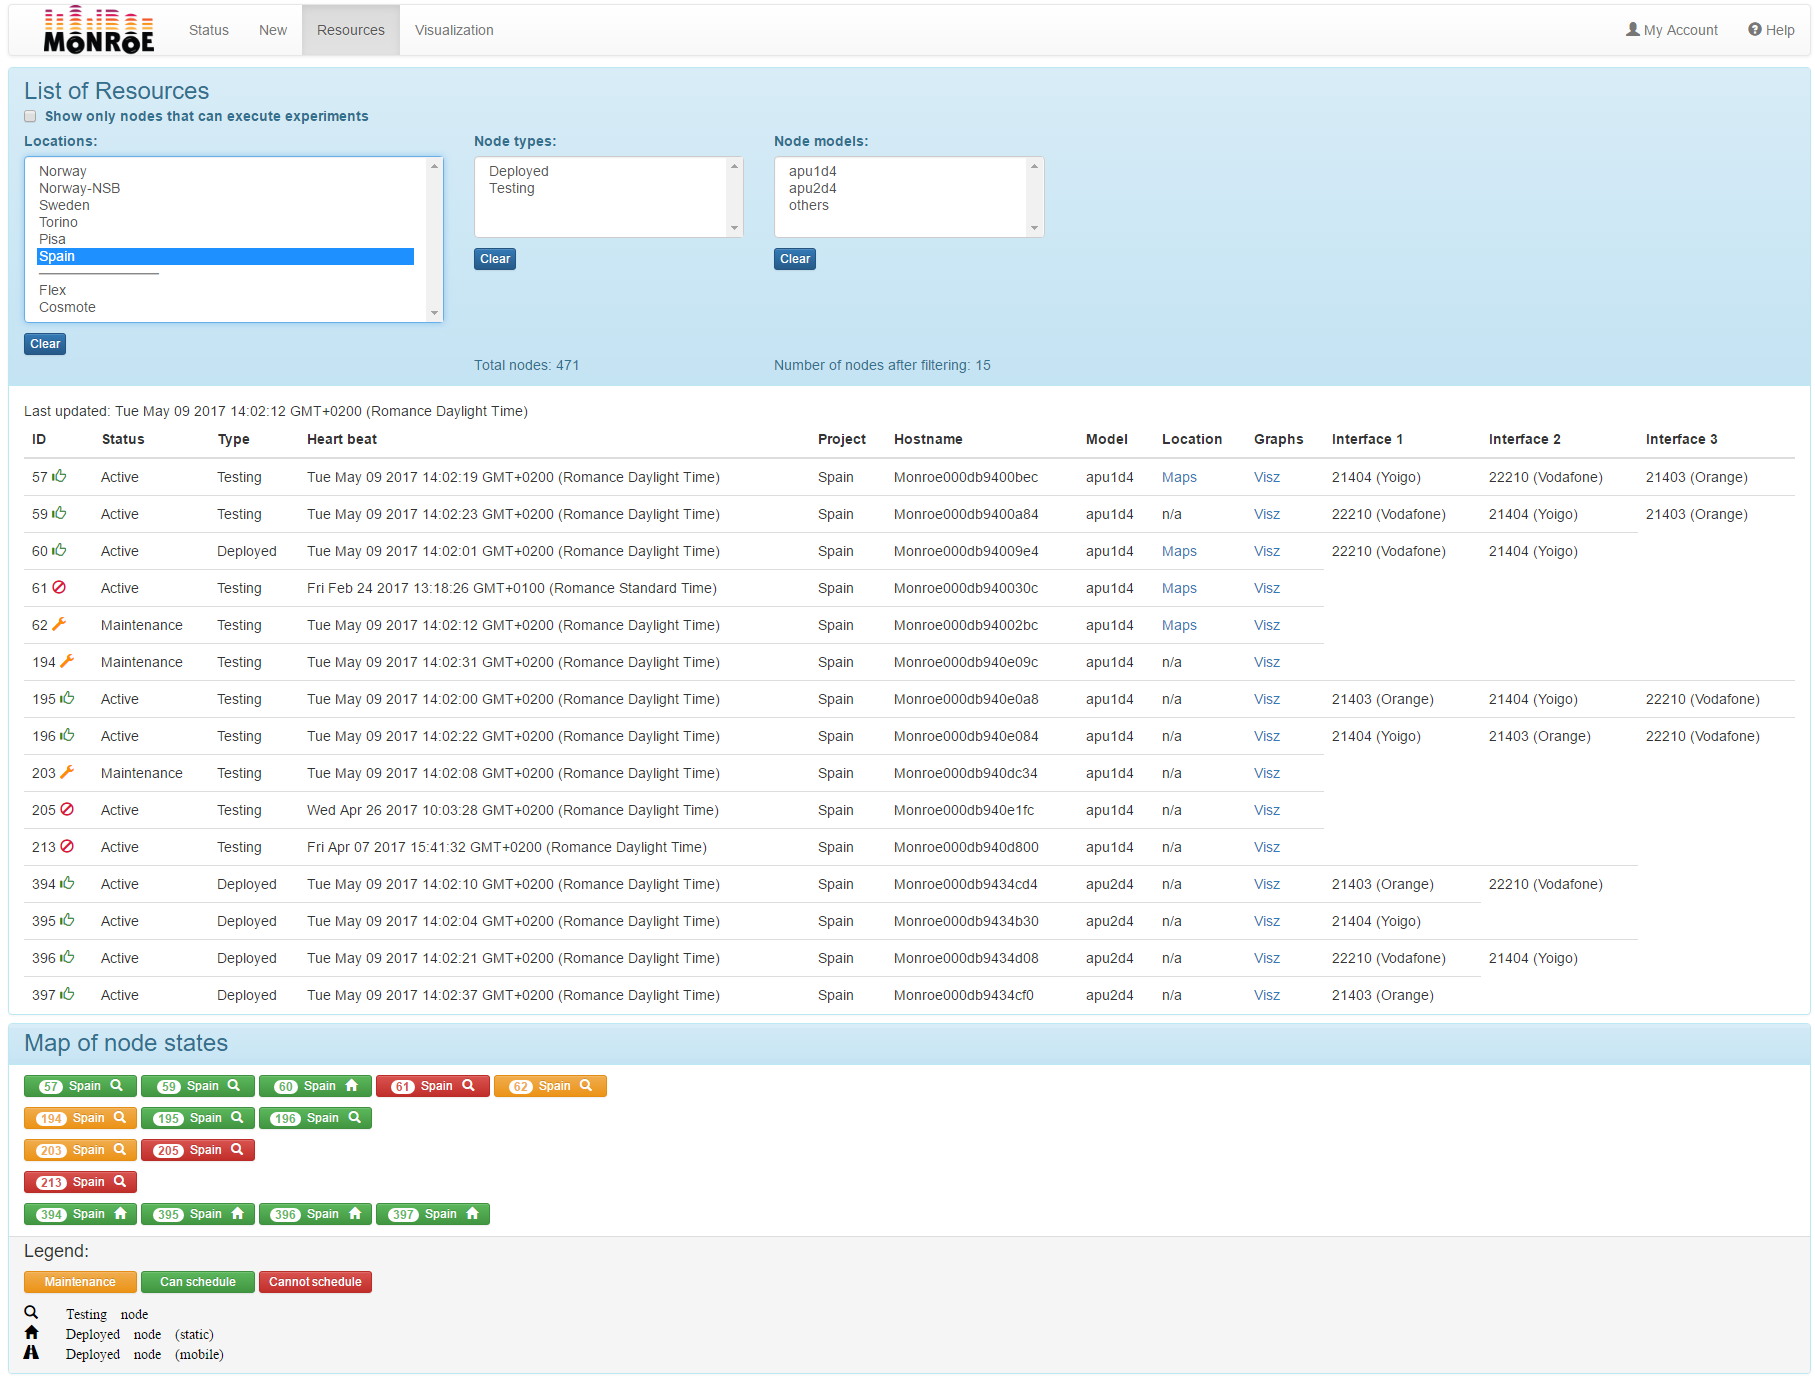
\includegraphics[width=1\textwidth]{Resources.png}
	\caption{Status of the \monroe{} nodes. The screen capture shows all types of nodes in Spain. The green approval sign (``thumbs-up'') close to the node IDs indicates that this node is capable of executing experiments. Clicking on the ``Location'' link for a node opens a Google Maps page showing the location of the node. Finally, the bottom part of the screen shows a ``map'' of nodes that allows users and \monroe{} administrators to quickly identify available (and problematic) nodes in the platform.}
	\label{fig:Resources}
\end{figure}


%------------------------------------------------------------%
%------------------------------------------------------------%
%------------------------------------------------------------%

\section{\monroe{} templates, examples and default experiments}
\label{sec:examples}

This section details the template for building \monroe{} experiments, the experiments that run as part of the default \monroe{} platform and several additional examples that can be directly used or that can serve as the basis for new ones.
The source code for the examples is publicly available at \url{https://github.com/MONROE-PROJECT/Experiments}.


%------------------------------------------------------------%
\subsection{Example template}
\label{subsec:exampleTemplate}

This experiment template provides an extensive example to show the capabilities of the \monroe{} platform.
The experiment will download a url (file) over http using \identifier{curl} from a configurable operator while at the same time recording the GPS positions of the node.
If the operator is not available at the time of execution, the experiment will fail.

\subsubsection{Usage}
\label{subsubsec:templateUsage}
%The default values are provided in the \identifier{/monroe/config} file.
%These values can be modified with the following two methods, where ``Additional options'' take precedence over the values specified in the configuration file:

%\begin{enumerate*}
%	\item Supplying your own \identifier{/monroe/config} file.
%	The file in your Docker layer will override the default file in the template docker layer.
%	The configured parameters will be fixed for all the executions of your container.
%	Notice that the whole file is substituted in the file system; hence, parameters not included in the configuration file of the user experiment will remain unspecified.
%	\item Supplying a JSON string in the ``Additional options'' field of the web user interface.
%	In this way, each execution of the experiment can receive a specific set of parameters.
%\end{enumerate*}

The configuration values can be supplied as a JSON string in the ``Additional options'' field of the web user interface.
This allows to specify a different set of parameters for each execution of the experiment.

The values of the configuration parameters can be read by the experiment from the \identifier{/monroe/config} file.
The following text shows a configuration file with %per-container and 
per-execution (``additional options'' field) options:%
\footnote{Entries in the \identifier{/monroe/config} file may appear in different order.}

{\VerbatimFont
	\begin{verbatim}
	{
	"stop": 1486653420, 
	"start": 1486653120,
	"traffic": 1048576,
	"script": "mikepeon/mike-depurar",
	"shared": 0,
	"storage": 134217728,
	"resultsQuota": 0,
	"guid": "sha256:3796f833f55c8dbca7e9845ea06120ccebec85c2770c0de2deb57509300efa44.165695.48.1",
	"option1": "value1",
	"option2": "value2",
	"nodeid": "48"
	}
	\end{verbatim}}

The default configuration values are as follows:

{\VerbatimFont
	\begin{verbatim}
	{
	# The following values are specific to the monroe platform
	"guid": "no.guid.in.config.file",              # Created by the scheduler
	"nodeid": "no.nodeid.in.config.file",          # Created by the scheduler
	"storage": 104857600,                          # Created by the scheduler
	"traffic": 104857600,                          # Created by the scheduler
	"script": "jonakarl/experiment-template",      # Created by the scheduler
	"zmqport": "tcp://172.17.0.1:5556",
	"modem_metadata_topic": "MONROE.META.DEVICE.MODEM",
	"gps_metadata_topic": "MONROE.META.DEVICE.GPS",
	# "dataversion": 1,                            # Version of the experiment
	# "dataid": "MONROE.EXP.JONAKARL.TEMPLATE",    # Name of the experiement
	"meta_grace": 120,                             # Grace period to wait for interface metadata
	"exp_grace": 120,                              # Grace period before killing experiment
	"meta_interval_check": 5,                      # Interval to check if interface is up
	"verbosity": 2,                                # 0="Mute", 1=error, 2=information, 3=verbose
	"resultdir": "/monroe/results/",
	# These values are specic for this experiment
	"operator": "Telenor SE",
	"url": "http://193.10.227.25/test/1000M.zip",
	"size": 3*1024 - 1,                            # The maximum size in Kbytes to download
	"time": 3600                                   # The maximum time in seconds for a download
	}
	\end{verbatim}}

The download will abort when either size OR time OR actual size of the ``url'' is downloaded.
All debug/error information will be printed on \identifier{stdout}, depending on the ``verbosity'' variable.

\subsubsection{Requirements}

The following directories and files must exist and have read and write permissions for the user/process running the container:

\begin{itemize*}
	\item \identifier{/monroe/config}, supplyed by the scheduler in the nodes.
	\item ``\identifier{resultdir},'' according to the values supplied in the configuration string or the default ones (Section~\ref{subsubsec:templateUsage}).
\end{itemize*}

\subsubsection{Output}

The experiment will execute a statement similar to running \identifier{curl} with the following command line:

{\VerbatimFont
	\begin{verbatim}
	curl -o /dev/null --raw --silent --write-out "{ remote: %{remote_ip}:%{remote_port},
	size: %{size_download}, speed: %{speed_download}, time: %{time_total},
	time_download: %{time_starttransfer} }" --interface eth0 --max-time 100 --range 0-100
	http://193.10.227.25/test/1000M.zip
	\end{verbatim}}

The experiment will produce a single-line JSON object similar to this (pretty printed to improve readability):

{\VerbatimFont
	\begin{verbatim}
	{
	"Bytes": 30720000,
	"DataId": "313.123213.123123.123123",
	"DataVersion": 1,
	"DownloadTime": 2.716,
	"GPSPositions": [
	{
	"Altitude": 225.0,
	"DataId": "MONROE.META.DEVICE.GPS",
	"DataVersion": 1,
	"Latitude": 59.404697,
	"Longitude": 13.581558,
	"NMEA": "$GPGGA,094832.0,5924.281896,N,01334.893500,E,1,05,1.6,225.0,M,35.0,M,,*5D\r\n",
	"SatelliteCount": 5,
	"SequenceNumber": 14,
	"Timestamp": 1465551728
	},
	{
	"DataId": "MONROE.META.DEVICE.GPS",
	"DataVersion": 1,
	"Latitude": 59.404697,
	"Longitude": 13.581558,
	"NMEA": "$GPRMC,094832.0,A,5924.281896,N,01334.893500,E,0.0,,100616,0.0,E,A*2B\r\n",
	"SequenceNumber": 15,
	"Timestamp": 1465551728
	}
	],
	"Guid": "sha256:15979bc2e2449b0011826c2bb8668df980da88221af3fc7916cb2eba4f2296c1.0.45.15",
	"Host": "193.10.227.25",
	"Iccid": "89460850007006922138",
	"InterfaceName": "usb0",
	"NodeId": "45",
	"Operator": "Telenor SE",
	"Port": "80",
	"SequenceNumber": 1,
	"SetupTime": 0.004,
	"Speed": 11295189.0,
	"TimeStamp": 1465551458.099917,
	"TotalTime": 2.72
	}
	\end{verbatim}}

\subsubsection{Overview of the code structure}

The experiment consists of one main process and two sub processes, where one process listens to modem and gps information, and the other executes the experiment.
The main process supervises the execution of its two children.

\paragraph{Information sharing between processes.}
Information is shared between processes via two thread-safe data structures (i.e., a Python ``Manager'' object).
Regarding modem information, the latest metadata update (for the specified operator) is stored in a dictionary.
The GPS information is continuously appended to a list as it is received.

\paragraph{The metadata sub-process.}
This process listens to GPS and modem messages sent on the ZeroMQ bus and updates the shared data structures.

\paragraph{The experiment sub-process.}
This process reads entries from the shared data structures, runs the experiment and saves its result when finished.

\subsection{Docker miscellaneous usage notes}

\begin{itemize*}
	\item List running containers:
	\begin{verbatim}docker ps\end{verbatim}
	
	\item Debug shell:
	\begin{verbatim}docker run -i -t --entrypoint bash --net=host template\end{verbatim}
	
	\item Normal execution with output to \identifier{stdout}:
	\begin{verbatim}docker run -i -t --net=host template\end{verbatim}
	
	\item Attach to a running container (with shell):
	\begin{verbatim}docker exec -i -t [container runtime name] bash\end{verbatim}
	
	\item Get container logs (\identifier{stderr} and \identifier{stdout}):
	\begin{verbatim}docker logs [container runtime name]\end{verbatim}
\end{itemize*}


%------------------------------------------------------------%
\subsection{Experiment: ping}

This background experiment runs continuously an RTT estimate on each MBB operator on the node (one independent experiment is run per interface).
The experiments measure IP RTT by continuously sending ping packets to a configurable server (by default \identifier{8.8.8.8}, Google's public DNS server).
The experiment will send one ``Echo Request'' (ICMP type 8) packet per second over the specified interface until aborted.
RTT is measured as the time between the echo request is sent and the echo reply (ICMP type 0) is received from the server.
The experiment runs on all interfaces in parallel.

\subsubsection{Usage}

The experiment is designed to run as a Docker container and will not attempt to do any active network configuration.
If the specified interface does not exist (i.e., is not up) when the experiment starts, it will immediately exit.

The default parameter values are:

{\VerbatimFont
	\begin{verbatim}
	{
	"guid": "no.guid.in.config.file",                # Created by the scheduler
	"zmqport": "tcp://172.17.0.1:5556",
	"nodeid": "fake.nodeid",
	"modem_metadata_topic": "MONROE.META.DEVICE.MODEM",
	"server": "8.8.8.8",                             # ping target
	"interval": 1000,                                # time in ms between successive packets
	"dataversion": 2,
	"dataid": "MONROE.EXP.PING",
	"meta_grace": 120,                               # Grace period to wait for interface metadata
	"ifup_interval_check": 5,                        # Interval to check if interface is up
	"export_interval": 5.0,
	"verbosity": 2,                                  # 0="Mute", 1=error, 2=Information, 3=verbose
	"resultdir": "/monroe/results/",
	"modeminterfacename": "InternalInterface",
	"interfacename": "eth0",                         # Interface to run the experiment on
	"interfaces_without_metadata": ["eth0", "wlan0"] # Manual metadata on these interfaces
	}
	\end{verbatim}}

All debug/error information will be printed on \identifier{stdout} depending on the value of the ``verbosity'' parameter.

\subsubsection{Requirements}

The following directories and files must exist and have read and write permissions for the user/process running the container:

\begin{itemize*}
	\item \identifier{/monroe/config}, supplyed by the scheduler in the nodes.
	\item ``\identifier{resultdir},'' according to the values supplied in the configuration string or the default ones (Section~\ref{subsubsec:templateUsage}).
\end{itemize*}

\subsubsection{Output}

The experiment will execute a statement similar to running \identifier{fping} with the following command line:

{\VerbatimFont
	\begin{verbatim}
	fping -I eth0 -D -c 1 -p 1000 -l 8.8.8.8
	\end{verbatim}}

The experiment will produce one of the two following single-line JSON objects, depending on whether it got a reply form the server or not.
If a reply was received:

{\VerbatimFont
	\begin{verbatim}
	{
	"Guid": "313.123213.123123.123123", # exp_config['guid']
	"Timestamp": 23123.1212, # time.time()
	"Iccid": 2332323, # meta_info["ICCID"]
	"Operator": "Telia", # meta_info["Operator"]
	"NodeId" : "9", # exp_config['nodeid']
	"DataId": "MONROE.EXP.PING",
	"DataVersion": 2,
	"SequenceNumber": 70,
	"Rtt": 6.47,
	"Bytes": 84,
	"Host": "8.8.8.8",
	}
	\end{verbatim}}

If the reply was not received (Bytes and RRR values are not present):

{\VerbatimFont
	\begin{verbatim}
	{
	"Guid": "313.123213.123123.123123", # exp_config['guid']
	"Timestamp": 23123.1212, # time.time()
	"Iccid": 2332323, # meta_info["ICCID"]
	"Operator": "Telia", # meta_info["Operator"]
	"NodeId" : "9", # exp_config['nodeid']
	"DataId": "MONROE.EXP.PING",
	"DataVersion": 2,
	"SequenceNumber": 71,
	"Host": "8.8.8.8",
	}
	\end{verbatim}}


%------------------------------------------------------------%
\subsection{Experiment: http\_download}

This is a periodically scheduled experiment that monitors the download speed of each MBB operator on the node.
The experiment will, over each MBB operator in sequence, download the specified url (file) with \identifier{curl} (http), presenting one result per interface.
The \monroe{} experiment template described in Section \ref{subsec:exampleTemplate} corresponds to this experiment, therefore, it is not further detailed here.


%------------------------------------------------------------%
\subsection{Experiment: Tstat \& mPlane}

The mPlane protocol provides control and data interchange for passive and active network measurement tasks.
It is built around a simple workflow that can interact with different frameworks to provide the results of the measurements.
This package includes an mPlane proxy and generic configuration files for Tstat.

mPlane captures traffic flow on all interfaces with the Tstat (\url{http://tstat.polito.it/}) probe.
The mPlane container is always running as one of the default experiments on all \monroe{} nodes.
The Tstat passive traces are stored locally on the node and are accessible by the experimenters.
A detailed description and the source code are available on github (\url{https://github.com/MONROE-PROJECT/mPlane}).

Tstat RRD logs and the compressed log are stored in the node at \identifier{/experiments/monroe/mplane}.
Tstat logs are transfered to the \monroe{} server and imported into \monroe{}'s (Cassandra) database.
The structure of the database tables is available on github (\url{https://github.com/MONROE-PROJECT/Database/blob/master/db_schema.cql}).

During experiment execution, the last three Tstat logs are shared with the experiment at \identifier{/monroe/tstat}.
Therefore, \monroe{} users can access the passive traces collected by Tstat during their experiments.

The data collected for a subset of the most relevant metrics for the HTTP experiments are visualized by the \monroe{} visualization tool.
And example of the metrics contained in the Tstat logs can be seen here: \url{http://213.182.68.136:8080/#/experiment/tstat}.

\subsubsection{Requirements}

The script must have access to \identifier{/nodeid} and run \identifier{get\_nodeid}.

\subsubsection{Usage}

Create your docker image normally and execute the container with the following command line:

{\VerbatimFont
	\begin{verbatim}
	docker run -i -t --net=host -d -v /mplane:/monroe/results -v /tstat:/monroe/tstat
	-v /etc/nodeid:/nodeid:ro monroe/mplane
	\end{verbatim}}


%------------------------------------------------------------%
\subsection{\monroe{} example: helloworld}

This experiment provides an easy example for using the configuration options from the scheduler, listen to and record the metadata stream (e.g., GPS and operator information), and show the experiment log functionality on a \monroe{} node.
The experiment listens to the metadata stream and records the \identifier{nr\_of\_messages} first messages.
The metadata messages are saved in JSON format with a custom field (``Hello'') in the output directory.
Additionally, the experiment prints out some debugging messages to show how these messages are logged and later retrieved via the web user interface.

\subsubsection{Usage}
\label{subsubsec:helloworldUsage}

The experiment is configured with a JSON string introduced via the ``Additional options'' field in the web user interface.
The configurable parameters and their default values are:

{\VerbatimFont
	\begin{verbatim}
	{
	"zmqport": "tcp://172.17.0.1:5556",
	"nodeid": "fake.nodeid",              # Needs to be overriden
	"metadata_topic": "MONROE.META",
	"verbosity": 2,                       # 0 = "Mute", 1=error, 2=Information, 3=verbose
	"resultdir": "/monroe/results/",
	"nr_of_messages": 3
	}
	\end{verbatim}}

\subsubsection{Requirements}

The following directories and files must exist and have read and write permissions for the user/process running the container:

\begin{itemize*}
	\item \identifier{/monroe/config}, supplyed by the scheduler in the nodes.
	\item ``\identifier{resultdir},'' according to the values supplied in the configuration string or the default ones (Section~\ref{subsubsec:helloworldUsage}).
\end{itemize*}

\subsubsection{Output}

The experiment will produce a single-line JSON object similar to the following ones, depending on the metadata received (``pretty printed'' here to improve readability):

{\VerbatimFont
	\begin{verbatim}
	{
	"DataId": "MONROE.META.NODE.SENSOR",
	"DataVersion": 1,
	"SequenceNumber": 58602,
	"Timestamp": 1465888420,
	"NodeId": "9",
	"Hello": "World"
	}
	\end{verbatim}}

\noindent The log file will contain records similar to these ones:

{\VerbatimFont
	\begin{verbatim}
	[2017-02-07 09:53:27.190338] Hello: Default config {
	"metadata_topic": "MONROE.META", 
	"nodeid": "fake.nodeid", 
	"nr_of_messages": 3, 
	"resultdir": "/monroe/results/", 
	"verbosity": 2, 
	"zmqport": "tcp://172.17.0.1:5556"
	}
	[2017-02-07 09:53:27.20000] Hello: Start recording messages with configuration {
	"metadata_topic": "MONROE.META", 
	"nodeid": "fake.nodeid", 
	"nr_of_messages": 3, 
	"resultdir": "/monroe/results/", 
	"verbosity": 2, 
	"zmqport": "tcp://172.17.0.1:5556"
	}
	[[2017-02-07 09:53:27.30000] Received message 1 with topic : MONROE.META.NODE.SENSOR
	{
	"DataId": "MONROE.META.NODE.SENSOR",
	"DataVersion": 1,
	"SequenceNumber": 58602,
	"Timestamp": 1465888420,
	"NodeId": "9",
	"Hello": "World"
	}
	. # And so on for each metadata message received until the configured value of metadata messages
	.
	.
	[2017-02-07 09:53:27.40000] Hello : Finished the experiment
	\end{verbatim}}


%------------------------------------------------------------%
\subsection{\monroe{} example: paris-traceroute}

This example showcases how to use the \monroe{}-modified version of paris-traceroute inside a container.
The binary of this tool is included in the base image of \monroe{}.

The original version of paris-traceroute has no option to choose which interface should be used.
In this version, flags to set the interface and source IP of the transmitted packets have been added.
Setting the interface is obligatory; if it is not set, the program will crash (by design), since if the interface were chosen automatically, it would probably not be what the experimenter intended to use.
The source IP flag is optional.
Just setting the IP flag to the IP of an interface without setting the interface flag will not work either.
This is done on purpose as well, as it might be possible for multiple interfaces to have the same IP within the \monroe{} network namespace.
If the IP flag is not set, the source IP is set to the IP of the chosen interface.

\subsubsection{Usage (inside a \monroe{} container)}

The parameters of this experiment are provided as ``Additional options'' in the scheduling web interface.
The following JSON string is an example of the additional options that can be passed to this container:
\begin{verbatim}
"interfaces": ["op1", "op2"], "targets": ["8.8.8.8", "www.uc3m.es"],
"traceAlgos": ["exh"], "protocol": "udp"
\end{verbatim}

Flags:
\begin{verbatim}
-C  --nodeIPArgument              Source IP
-O  --nodeInterfaceArgument       Source interface (mandatory)
\end{verbatim}

The paris-traceroute binary can be executed (as any normal Linux command) either without specifying a traceroute algorithm to perform a ``simple'' traceroute (similar to the output of the ordinary traceroute command), or with the flags \identifier{-n -a exh}, to perform an exhaustive traceroute.
Exhaustive traceroutes provide more detailed and accurate paths between the host (\monroe{} node) and the target server that are able to detect, among others, the presence of load balancers, which create multiple paths between host and target.

\subsubsection{Output}

The experiment output is a text file:

{\VerbatimFont
	\begin{verbatim}
	root@b59e69a56297:/# paris-traceroute -O op2 -C 192.168.1.127 8.8.8.8
	traceroute [(192.168.1.127:33456) -> (8.8.8.8:33457)], protocol udp, algo hopbyhop, duration 18 s
	1  192.168.1.1 (192.168.1.1)  2.946 ms   0.553 ms   0.559 ms 
	2  * * *
	3  10.133.17.29 (10.133.17.29)  83.259 ms   136.577 ms   82.050 ms 
	4  10.133.17.14 (10.133.17.14)  78.783 ms   131.510 ms   79.231 ms 
	5  10.133.17.236 (10.133.17.236)  84.243 ms   133.024 ms   79.785 ms 
	6  10.133.17.3 (10.133.17.3)  81.543 ms   139.381 ms   100.263 ms 
	7  83.224.40.186 (83.224.40.186)  89.319 ms   188.926 ms   179.963 ms 
	MPLS Label 24703 TTL=254
	8  83.224.40.185 (83.224.40.185)  82.710 ms   172.438 ms   147.020 ms 
	9  85.205.14.105 (85.205.14.105)  85.179 ms   137.514 ms   125.869 ms 
	10  72.14.223.169 (72.14.223.169)  85.609 ms   137.363 ms   118.063 ms 
	11  216.239.47.128 (216.239.47.128)  79.567 ms   146.356 ms   145.285 ms 
	12  209.85.243.33 (209.85.243.33)  129.615 ms   198.938 ms   269.407 ms 
	MPLS Label 568892 TTL=1
	13  64.233.174.143 (64.233.174.143)  108.599 ms   185.810 ms   246.661 ms 
	MPLS Label 692130 TTL=1
	14  108.170.234.47 (108.170.234.47)  111.645 ms   825.615 ms   1424.942 ms 
	15  * * *
	16  google-public-dns-a.google.com (8.8.8.8)  103.087 ms !T2   166.279 ms !T2   224.649 ms !T2 
	\end{verbatim}
}


\subsubsection{Additional remarks}

Paris-traceroute instances should be run sequentially and preferably when the node is generating little traffic in general because it uses raw packet capture to detect the replies from intermediate nodes and background traffic might interfere with this process.


%------------------------------------------------------------%
\subsection{\monroe{} example: headlessbrowsing}

This experiment evaluates the performance of different HTTP protocols (HTTP1.1, HTTP1.1/TLS, HTTP2) using the headless Firefox browser.
It uses the Selenium browser-automation framework, which enables execution of web-browsing automation tests in different browsers such as Firefox and Chrome.
The Selenium web-driver is used for Firefox.
For a given url, HTTP protocol and source network interface, Selenium launches the native Firefox browser to visit that url.

\subsubsection{Output}
This experiment generates an HTTP ARchive (HAR) file during the download of a target url that helps to find afterwards the impact of different web-page features on its overall Page Load Time (PLT).

The experiment generates a single JSON file such as:

{\VerbatimFont
	\begin{verbatim}
	{
	"DataId":"MONROE.EXP.FIREFOX.HEADLESS.BROWSING",
	"ping_min":" 55.6",
	"ping_max":"56.8",
	"NumObjects":6,
	"InterfaceName":"usb2",
	"Web load time":196,
	"PageSize":35641,
	"DataVersion":1,
	"Timestamp":1481536829.0814,
	"NWMCCMNC":22210,
	"Objects":[
	{
	"objectSize":1951,
	"mimeType":"image/png",
	"startedDateTime":"2016-12-12T10:00:21.293+00:00",
	"url":"https://www.wikipedia.org/portal/wikipedia.org/assets/img/Wikipedia_wordmark.png",
	"timings":{"receive":1, "send":0, "connect":1, "dns":0, "blocked":0, "wait":60},
	"time":62
	},
	{
	"objectSize":13196,
	"mimeType":"image/png",
	"startedDateTime":"2016-12-12T10:00:21.294+00:00",
	"url":"https://www.wikipedia.org/portal/wikipedia.org/assets/img/Wikipedia-logo-v2.png",
	"timings":{"receive":52, "send":3, "connect":59, "dns":2, "blocked":0, "wait":53 },
	"time":169
	},
	{
	"objectSize":9425,
	"mimeType":"application/javascript",
	"startedDateTime":"2016-12-12T10:00:21.295+00:00",
	"url":"https://www.wikipedia.org/portal/wikipedia.org/assets/js/index-abc278face.js",
	"timings":{"receive":3, "send":0, "connect":120, "dns":0, "blocked":0, "wait":65},
	"time":188
	},
	{
	"objectSize":1164,
	"mimeType":"application/javascript",
	"startedDateTime":"2016-12-12T10:00:21.296+00:00",
	"url":"https://www.wikipedia.org/portal/wikipedia.org/assets/js/gt-ie9-c84bf66d33.js",
	"timings":{"receive":0, "send":1, "connect":64, "dns":2, "blocked":0, "wait":70 },
	"time":137
	},
	{
	"objectSize":1590,
	"mimeType":"image/png",
	"startedDateTime":"2016-12-12T10:00:21.381+00:00",
	"url":"https://www.wikipedia.org/portal/wikipedia.org/assets/img/sprite-icons.png?
	27378e2bb51199321b32dd1ac3f5cd755adc21a5",
	"timings":{"receive":1, "send":0, "connect":1, "dns":0, "blocked":0, "wait":49 },
	"time":51
	},
	{
	"objectSize":8315,
	"mimeType":"image/png",
	"startedDateTime":"2016-12-12T10:00:21.425+00:00",
	"url":"https://www.wikipedia.org/portal/wikipedia.org/assets/img/sprite-project-logos.png?
	dea6426c061216dfcba1d2d57d33f4ee315df1c2",
	"timings":{"receive":2, "send":0, "connect":8, "dns":0, "blocked":0, "wait":54 },
	"time":64
	} ],
	"IPAddress":"2.43.181.254",
	"IMSIMCCMNC":22210,
	"tracedRoutes":["192.168.96.1", "193.10.227.25", "xx.xx.xx.xx" ..... "192.168.96.1" ],
	"InternalInterface":"op0",
	"NodeId":"41",
	"ping_exp":1,
	"Protocol":"HTTP1.1",
	"SequenceNumber":1,
	"url":"www.wikipedia.org",
	"ping_avg":"56.2",
	"InternalIPAddress":"192.168.96.123",
	"Operator":"voda IT",
	"Iccid":"8939104160000392116"
	}
	\end{verbatim}}

%------------------------------------------------------------%
\subsection{\monroe{} example: pReplay}

The pReplay experiment replays the dependency graph of a web site.

The traversal begins with the first activity: Loading the root HTML.
After building the dependency graph, it acts for each task whose dependencies have already been met.
For network tasks, it makes a request for the corresponding url; correspondingly, for computation activities, it waits for the amount of time mentioned in the graph.
Once a particular activity is finished, pReplay checks if any activities depending on that one have already met all of their dependencies and must thus be triggered.
pReplay walks through the dependency graph until all activities in the graph have been visited.

\subsubsection{Usage}

Execute pReplay on a command line inside a container as with any other Linux command:
{\VerbatimFont
	\begin{verbatim}
	./pReplay interface_name server testfile [http|https|http2] [max-connections] [cookie-size]
	\end{verbatim}}

\noindent Parameters:
\begin{itemize*}
	\item \textbf{interface\_name:} Source interface for outgoing traffic.
	\item \textbf{server:} DNS name or IP address.
	\item \textbf{testfile:} Relative path to test file in JSON format.
	\item \textbf{protocol:}
	\begin{itemize*}
		\item http: http 1.1
		\item https: http 1.1 with SSL
		\item http2: http 2
	\end{itemize*}
	\item \textbf{max-connections:} Maximum amount of concurrent connections.
	\item \textbf{cookie-size:} Size of cookie --- works with http1 only.
\end{itemize*}


%------------------------------------------------------------%
\subsection{\monroe{} example: astream}

AStream is a Python based emulated video player to evaluate the performance of the DASH bitrate adaptation algorithms.
The supported rate adaptation algorithms are:

\begin{itemize*}
	\item Basic adaptation.
	\item Segment Aware Rate Adaptation (SARA)~\cite{p:juluri2015}.
	\item Buffer-Based Rate Adaptation (Netflix)~\cite{p:teyuan2014}.
\end{itemize*}

\subsubsection{Usage}

The experimenter can choose the rate adaptation algorithm passing a JSON string to the scheduler through the user interface (e.g., \identifier{"playback":"NETFLIX"}).
The default is the basic adaptation scheme.
Additionally, the user can specify the target MPD file to play (e.g., \identifier{"mpd\_file":"http://128.39.37.161:8080/BigBuck\-Bunny\_4s.mpd"}) and the number of segments to retrieve (e.g., \identifier{"segment\_limit":10}).

\subsubsection{Output}

The astream container outputs two log files:
\begin{enumerate*}
	\item Buffer logs: Epoch time, current playback time, current buffer size (in segments), current playback state.
	\item Playback logs: Epoch time, playback time, segment number, segment size, playback bitrate, segment duration, weighted harmonic mean average download rate.
\end{enumerate*}


%------------------------------------------------------------%
\subsection{\monroe{} example: udpbwestimator}

Udpbwestimator is an experiment setup to estimate available bandwidth for a particular network interface.
It consists of two applications, a receiver and a traffic generator (server).
The receiver initiates connections and requests the server for traffic.
Then, every second, the server sends a burst of UDP packets back to back to the receiver, which follows the packet arrival times and estimates the available bandwidth.

\subsubsection{Usage}

The receiver accepts the following command line parameters:
\begin{itemize*}
	\item[] -c : Number of back-to-back packets to be sent in each second.
	\item[] -b : Number of bursts to be sent.
	\item[] -l : Payload length in bytes.
	\item[] -s : Source IP to bind to.
	\item[] -o : Source port.
	\item[] -d : Destination IP.
	\item[] -p : Destination port.
	\item[] -w : Optional, filename for writing the packet arrival times.
\end{itemize*}

\subsubsection{Output}

The experiment will produce a single-line JSON object similar to the following:

{\VerbatimFont
	\begin{verbatim}
	{
	"CID" : 33346602,
	"DataId" : "MONROE.EXP.UDPBWESTIMATOR",
	"DataVersion" : 1,
	"DeviceMode" : 5,
	"DeviceState" : 3,
	"Guid" : "sha256:872af8c8b8f1635be6936a111b5fa838071e6f42cb317e9db1d9bb0c7db31425.93321.204.1",
	"IMEI" : "864154023639966",
	"IMSI" : "240016025247086",
	"IMSIMCCMNC" : 24001,
	"IPAddress" : "78.79.63.124",
	"Iccid" : "89460120151010468086",
	"InterfaceName" : "usb0",
	"InternalIPAddress" : "192.168.68.118",
	"InternalInterface" : "op1",
	"LAC" : 2806,
	"NWMCCMNC" : 24202,
	"NodeId" : "204",
	"Operator" : "NetCom",
	"RSRP" : -72,
	"RSRQ" : -7,
	"RSSI" : -49,
	"SequenceNumber" : 1,
	"Timestamp" : 1479312368.633218,
	"bw" : "48.41 38.98 36.44 50.00 30.20 45.21 47.02 37.89 44.37 28.90 25.91 38.57 48.74 
	39.94 43.37 37.94 43.81 39.60 52.00 47.55 48.20 34.85 41.44 47.60 57.26 46.11 
	45.66 52.04 37.43 49.67 33.56 50.35 41.11 51.63 45.33 104.01 45.73 49.95 50.37 
	38.57 29.45 50.95 54.95 45.42 47.13 34.30 46.10 103.68 79.75 45.72 52.03 30.38 
	50.21 36.96 71.51 54.66 39.26 44.12 45.18 39.93"
	}
	\end{verbatim}}


%------------------------------------------------------------%
\subsection{\monroe{} example: traceroute\_background\_experiment}

Performs traceroute periodically to various targets.
This experiment is meant to be run in the background and can be run in parallel with experiments of other users.
It uses the default traceroute binary distributed by the Debian repositories.

Each traceroute produces a text file that is parsed by \identifier{outputParser.py} to generate the JSON output of this experiment.
The JSON file is then imported into the \monroe{} database.

\subsubsection{Usage}

To reduce experiment duration, the traceroutes can be run in parallel.
The number of parallel traceroute instances is dictated by the \identifier{maxNumberOfTotalTracerouteInstances} parameter.
It is possible to parallelize on a per-interface basis (i.e., \identifier{maxNumberOfTotalTracerouteInstances} per interface) or per the whole experiment (i.e., \identifier{maxNumberOfTotalTracerouteInstances} total in the experiment instance spread among all the interfaces).
This behavior is controlled by the \identifier{executionMode} parameter.
The available options are: serially, serialPerInterface and parallel.

Additionally, a flag can be provided to choose the protocol of the probes: default, udp, tcp and icmp.

The parameters of this experiment are provided as ``Additional options'' in the web user interface.
An example JSON string that can be used with this container as additional options is:

{\VerbatimFont
	\begin{verbatim}
	"interfaces": ["op0", "op1", "op2"], "targets": ["www.ntua.gr", "www.uc3m.es", "Google.com", 
	"Facebook.com", "Youtube.com", "Baidu.com", "Yahoo.com", "Amazon.com", "Wikipedia.org", 
	"audio-ec.spotify.com", "mme.whatsapp.net", "sync.liverail.com", "ds.serving-sys.com", 
	"instagramstatic-a.akamaihd.net"], "maxNumberOfTotalTracerouteInstances": 5, 
	"executionMode": "parallel"
	\end{verbatim}}


%------------------------------------------------------------%
\subsection{Other containers in the repositories}

Our public repositories contain the source code for other Docker containers that perform varied tasks in the nodes.
Although they are not intended as examples, users can take a look into them to gain a deeper understanding of the platform configuration. 

\subsubsection{Container: metadata-subscriber}

The subscriber is designed to listen to ZMQ messages send out by the metadata-multicaster.
The subscriber attaches to a configurable ZeroMQ socket and listens to all messages that begin with the topic ``MONROE.META,'' except the ones whose topic ends with ``.UPDATE'' (rebroadcasts) and/or begins with ``MONROE.META.DEVICE.CONNECTIVITY.'' as these are redundant.
All messages are updated with NodeId, but are otherwise saved verbatim as a JSON formatted file suitable for later import in the \monroe{} databases.

\subsubsection{Container: tunnelbox-server}

This container acts as an SSH reverese tunnel endpoint that clients can use to directly connect to their experiment containers (on any \monroe{} node).
The purpose is to provide experimenters an interactive way of accessing an experiment running on a real \monroe{} node during development or debugging. 
The client has to supply its own public SSH key to the experiment container using the web user interface.
The web user interface provides further instructions (SSH command line) to connect to the experiment container using the provided key.

\subsubsection{Container: monroe\_base}

This is the container upon which all user experiments \emph{must} be built.
The container is based on Debian ``jessie'' with (\monroe{}) common experiment tools added.
For a list of the tools currently installed see the folder \identifier{monroe\_base.docker} in our repositories.


%------------------------------------------------------------%
%------------------------------------------------------------%
%------------------------------------------------------------%

\section{List of known bugs and issues}

\begin{itemize}
	
	\item In general, Firefox does not render the date-time picker correctly. You will have to either enter the dates and times manually or use Chrome.
	\item Container deployment can take several minutes, particularly for nodes without an Ethernet management connection (e.g., mobile nodes in trains or buses). When scheduling an experiment, the user has to take into account the time needed for the deployment. The system will not automatically take care of this at this moment.
	\item Similarly, the button ``Check availability'' returns the earliest available slot. However, it does not account for the time needed to deploy the container. The user must manually account for that.
	\item Checking the option ``ASAP'' to schedule an experiment as soon as possible may fail due to lack of time to deploy the container. The system does add some slack in this case, but its length may need some adjustment according to the type of nodes and MBB characteristics.
\end{itemize}

%------------------------------------------------------------%
%------------------------------------------------------------%
%------------------------------------------------------------%

\begin{appendices}
\section{List of packages installed in monroe/base}
\label{app:installedPackages}

{\scriptsize
\begin{longtable}{p{3.25cm}@{\hspace{0.25cm}}p{4cm}@{\hspace{0.25cm}}l@{\hspace{0.25cm}}p{7cm}}
	\caption{List of packages installed in \identifier{monroe/base} as of 2017-02-27.}\label{tab:installedPackages}\\
	\toprule
	\textbf{Name} & \textbf{Version} & \textbf{Architecture} & \textbf{Description} \\	\midrule
	\endfirsthead
	\caption{List of packages installed in \identifier{monroe/base}. (Continued)}\\
	\toprule
	\textbf{Name} & \textbf{Version} & \textbf{Architecture} & \textbf{Description} \\	\midrule
	\endhead
%
acl	&	2.2.52-2	&	amd64	&	Access control list utilities	\\
adduser	&	3.113+nmu3	&	all	&	add and remove users and groups	\\
adwaita-icon-theme	&	3.14.0-2	&	all	&	default icon theme of GNOME	\\
apt	&	1.0.9.8.4	&	amd64	&	commandline package manager	\\
base-files	&	8+deb8u6	&	amd64	&	Debian base system miscellaneous files	\\
base-passwd	&	3.5.37	&	amd64	&	Debian base system master password and group files	\\
bash	&	4.3-11+b1	&	amd64	&	GNU Bourne Again SHell	\\
bsdutils	&	1:2.25.2-6	&	amd64	&	basic utilities from 4.4BSD-Lite	\\
bzip2	&	1.0.6-7+b3	&	amd64	&	high-quality block-sorting file compressor - utilities	\\
ca-certificates	&	20141019+deb8u1	&	all	&	Common CA certificates	\\
ca-certificates-java	&	20140324	&	all	&	Common CA certificates (JKS keystore)	\\
coreutils	&	8.23-4	&	amd64	&	GNU core utilities	\\
curl	&	7.38.0-4+deb8u5	&	amd64	&	command line tool for transferring data with URL syntax	\\
d-itg	&	2.8.1-r1023-3	&	amd64	&	Distributed Internet Traffic Generator	\\
dash	&	0.5.7-4+b1	&	amd64	&	POSIX-compliant shell	\\
dbus	&	1.8.20-0+deb8u1	&	amd64	&	simple interprocess messaging system (daemon and utilities)	\\
dconf-gsettings-backend:amd64	&	0.22.0-1	&	amd64	&	simple configuration storage system - GSettings back-end	\\
dconf-service	&	0.22.0-1	&	amd64	&	simple configuration storage system - D-Bus service	\\
debconf	&	1.5.56	&	all	&	Debian configuration management system	\\
debconf-i18n	&	1.5.56	&	all	&	full internationalization support for debconf	\\
debian-archive-keyring	&	2014.3	&	all	&	GnuPG archive keys of the Debian archive	\\
debianutils	&	4.4+b1	&	amd64	&	Miscellaneous utilities specific to Debian	\\
default-jre-headless	&	2:1.7-52	&	amd64	&	Standard Java or Java compatible Runtime (headless)	\\
dh-python	&	1.20141111-2	&	all	&	Debian helper tools for packaging Python libraries and applications	\\
diffutils	&	1:3.3-1+b1	&	amd64	&	File comparison utilities	\\
dmsetup	&	2:1.02.90-2.2+deb8u1	&	amd64	&	Linux Kernel Device Mapper userspace library	\\
dpkg	&	1.17.27	&	amd64	&	Debian package management system	\\
dumb-init	&	1.2.0	&	amd64	&	wrapper script which proxies signals to a child	\\
e2fslibs:amd64	&	1.42.12-2	&	amd64	&	ext2/ext3/ext4 file system libraries	\\
e2fsprogs	&	1.42.12-2	&	amd64	&	ext2/ext3/ext4 file system utilities	\\
findutils	&	4.4.2-9+b1	&	amd64	&	utilities for finding files--find, xargs	\\
flent	&	0.15.0-1	&	all	&	The FLExible Network Tester	\\
fontconfig	&	2.11.0-6.3+deb8u1	&	amd64	&	generic font configuration library - support binaries	\\
fontconfig-config	&	2.11.0-6.3+deb8u1	&	all	&	generic font configuration library - configuration	\\
fonts-dejavu-core	&	2.34-1	&	all	&	Vera font family derivate with additional characters	\\
fping	&	3.10-2	&	amd64	&	sends ICMP ECHO\_REQUEST packets to network hosts	\\
gcc-4.8-base:amd64	&	4.8.4-1	&	amd64	&	GCC, the GNU Compiler Collection (base package)	\\
gcc-4.9-base:amd64	&	4.9.2-10	&	amd64	&	GCC, the GNU Compiler Collection (base package)	\\
glib-networking:amd64	&	2.42.0-2	&	amd64	&	network-related giomodules for GLib	\\
glib-networking-common	&	2.42.0-2	&	all	&	network-related giomodules for GLib - data files	\\
glib-networking-services	&	2.42.0-2	&	amd64	&	network-related giomodules for GLib - D-Bus services	\\
gnupg	&	1.4.18-7+deb8u3	&	amd64	&	GNU privacy guard - a free PGP replacement	\\
gpgv	&	1.4.18-7+deb8u3	&	amd64	&	GNU privacy guard - signature verification tool	\\
gpsd	&	3.11-3	&	amd64	&	Global Positioning System - daemon	\\
gpslogger-oml2	&	2.11.0-mytestbed2	&	amd64	&	Record and store GPS measurements using OML	\\
grep	&	2.20-4.1	&	amd64	&	GNU grep, egrep and fgrep	\\
gsettings-desktop-schemas	&	3.14.1-1	&	all	&	GSettings desktop-wide schemas	\\
gzip	&	1.6-4	&	amd64	&	GNU compression utilities	\\
hicolor-icon-theme	&	0.13-1	&	all	&	default fallback theme for FreeDesktop.org icon themes	\\
hostname	&	3.15	&	amd64	&	utility to set/show the host name or domain name	\\
httperf-oml2	&	2.11.0-mytestbed2	&	amd64	&	HTTP server performance tester, with OML support	\\
httping	&	1.5.8-1	&	amd64	&	ping-like program for http-requests	\\
inetutils-ping	&	2:1.9.2.39.3a460-3	&	amd64	&	ICMP echo tool	\\
init	&	1.22	&	amd64	&	System-V-like init utilities - metapackage	\\
init-system-helpers	&	1.22	&	all	&	helper tools for all init systems	\\
initscripts	&	2.88dsf-59	&	amd64	&	scripts for initializing and shutting down the system	\\
insserv	&	1.14.0-5	&	amd64	&	boot sequence organizer using LSB init.d script dependency information	\\
iperf	&	2.0.5+dfsg1-2	&	amd64	&	Internet Protocol bandwidth measuring tool	\\
iperf-oml2	&	2.11.0-mytestbed2	&	amd64	&	Internet Protocol bandwidth measuring tool, with OML support	\\
iperf3	&	3.0.7-1	&	amd64	&	Internet Protocol bandwidth measuring tool	\\
iproute2	&	3.16.0-2	&	amd64	&	networking and traffic control tools	\\
iptables	&	1.4.21-2+b1	&	amd64	&	administration tools for packet filtering and NAT	\\
java-common	&	0.52	&	all	&	Base of all Java packages	\\
jq	&	1.4-2.1	&	amd64	&	lightweight and flexible command-line JSON processor	\\
libacl1:amd64	&	2.2.52-2	&	amd64	&	Access control list shared library	\\
libapt-pkg4.12:amd64	&	1.0.9.8.4	&	amd64	&	package management runtime library	\\
libasound2:amd64	&	1.0.28-1	&	amd64	&	shared library for ALSA applications	\\
libasound2-data	&	1.0.28-1	&	all	&	Configuration files and profiles for ALSA drivers	\\
libasyncns0:amd64	&	0.8-5	&	amd64	&	Asynchronous name service query library	\\
libatk-bridge2.0-0:amd64	&	2.14.0-2	&	amd64	&	AT-SPI 2 toolkit bridge - shared library	\\
libatk1.0-0:amd64	&	2.14.0-1	&	amd64	&	ATK accessibility toolkit	\\
libatk1.0-data	&	2.14.0-1	&	all	&	Common files for the ATK accessibility toolkit	\\
libatspi2.0-0:amd64	&	2.14.0-1	&	amd64	&	Assistive Technology Service Provider Interface - shared library	\\
libattr1:amd64	&	1:2.4.47-2	&	amd64	&	Extended attribute shared library	\\
libaudit-common	&	1:2.4-1	&	all	&	Dynamic library for security auditing - common files	\\
libaudit1:amd64	&	1:2.4-1+b1	&	amd64	&	Dynamic library for security auditing	\\
libavahi-client3:amd64	&	0.6.31-5	&	amd64	&	Avahi client library	\\
libavahi-common-data:amd64	&	0.6.31-5	&	amd64	&	Avahi common data files	\\
libavahi-common3:amd64	&	0.6.31-5	&	amd64	&	Avahi common library	\\
libblas-common	&	1.2.20110419-10	&	amd64	&	Dependency package for all BLAS implementations	\\
libblas3	&	1.2.20110419-10	&	amd64	&	Basic Linear Algebra Reference implementations, shared library	\\
libblkid1:amd64	&	2.25.2-6	&	amd64	&	block device id library	\\
libbluetooth3:amd64	&	5.23-2+b1	&	amd64	&	Library to use the BlueZ Linux Bluetooth stack	\\
libbsd0:amd64	&	0.7.0-2	&	amd64	&	utility functions from BSD systems - shared library	\\
libbz2-1.0:amd64	&	1.0.6-7+b3	&	amd64	&	high-quality block-sorting file compressor library - runtime	\\
libc-bin	&	2.19-18+deb8u6	&	amd64	&	GNU C Library: Binaries	\\
libc6:amd64	&	2.19-18+deb8u6	&	amd64	&	GNU C Library: Shared libraries	\\
libcairo-gobject2:amd64	&	1.14.0-2.1+deb8u1	&	amd64	&	Cairo 2D vector graphics library (GObject library)	\\
libcairo2:amd64	&	1.14.0-2.1+deb8u1	&	amd64	&	Cairo 2D vector graphics library	\\
libcap-ng0:amd64	&	0.7.4-2	&	amd64	&	An alternate POSIX capabilities library	\\
libcap2:amd64	&	1:2.24-8	&	amd64	&	POSIX 1003.1e capabilities (library)	\\
libcap2-bin	&	1:2.24-8	&	amd64	&	POSIX 1003.1e capabilities (utilities)	\\
libcgi-fast-perl	&	1:2.04-1	&	all	&	CGI subclass for work with FCGI	\\
libcgi-pm-perl	&	4.09-1	&	all	&	module for Common Gateway Interface applications	\\
libcolord2:amd64	&	1.2.1-1+b2	&	amd64	&	system service to manage device colour profiles -- runtime	\\
libcomerr2:amd64	&	1.42.12-2	&	amd64	&	common error description library	\\
libconfig-grammar-perl	&	1.10-2	&	all	&	grammar-based user-friendly config parser	\\
libcroco3:amd64	&	0.6.8-3+b1	&	amd64	&	Cascading Style Sheet (CSS) parsing and manipulation toolkit	\\
libcryptsetup4:amd64	&	2:1.6.6-5	&	amd64	&	disk encryption support - shared library	\\
libcups2:amd64	&	1.7.5-11+deb8u1	&	amd64	&	Common UNIX Printing System(tm) - Core library	\\
libcurl3:amd64	&	7.38.0-4+deb8u5	&	amd64	&	easy-to-use client-side URL transfer library (OpenSSL flavour)	\\
libdatrie1:amd64	&	0.2.8-1	&	amd64	&	Double-array trie library	\\
libdb5.3:amd64	&	5.3.28-9	&	amd64	&	Berkeley v5.3 Database Libraries [runtime]	\\
libdbi1:amd64	&	0.9.0-4	&	amd64	&	DB Independent Abstraction Layer for C -- shared library	\\
libdbus-1-3:amd64	&	1.8.20-0+deb8u1	&	amd64	&	simple interprocess messaging system (library)	\\
libdbus-glib-1-2:amd64	&	0.102-1	&	amd64	&	simple interprocess messaging system (GLib-based shared library)	\\
libdconf1:amd64	&	0.22.0-1	&	amd64	&	simple configuration storage system - runtime library	\\
libdebconfclient0:amd64	&	0.192	&	amd64	&	Debian Configuration Management System (C-implementation library)	\\
libdevmapper1.02.1:amd64	&	2:1.02.90-2.2+deb8u1	&	amd64	&	Linux Kernel Device Mapper userspace library	\\
libdigest-hmac-perl	&	1.03+dfsg-1	&	all	&	module for creating standard message integrity checks	\\
libdrm2:amd64	&	2.4.58-2	&	amd64	&	Userspace interface to kernel DRM services -- runtime	\\
libedit2:amd64	&	3.1-20140620-2	&	amd64	&	BSD editline and history libraries	\\
libencode-locale-perl	&	1.03-1	&	all	&	utility to determine the locale encoding	\\
libexpat1:amd64	&	2.1.0-6+deb8u3	&	amd64	&	XML parsing C library - runtime library	\\
libfcgi-perl	&	0.77-1+b1	&	amd64	&	helper module for FastCGI	\\
libffi6:amd64	&	3.1-2+b2	&	amd64	&	Foreign Function Interface library runtime	\\
libfile-listing-perl	&	6.04-1	&	all	&	module to parse directory listings	\\
libflac8:amd64	&	1.3.0-3	&	amd64	&	Free Lossless Audio Codec - runtime C library	\\
libfontconfig1:amd64	&	2.11.0-6.3+deb8u1	&	amd64	&	generic font configuration library - runtime	\\
libfontenc1:amd64	&	1:1.1.2-1+b2	&	amd64	&	X11 font encoding library	\\
libfreetype6:amd64	&	2.5.2-3+deb8u1	&	amd64	&	FreeType 2 font engine, shared library files	\\
libgcc1:amd64	&	1:4.9.2-10	&	amd64	&	GCC support library	\\
libgcrypt20:amd64	&	1.6.3-2+deb8u2	&	amd64	&	LGPL Crypto library - runtime library	\\
libgdbm3:amd64	&	1.8.3-13.1	&	amd64	&	GNU dbm database routines (runtime version)	\\
libgdk-pixbuf2.0-0:amd64	&	2.31.1-2+deb8u5	&	amd64	&	GDK Pixbuf library	\\
libgdk-pixbuf2.0-common	&	2.31.1-2+deb8u5	&	all	&	GDK Pixbuf library - data files	\\
libgfortran3:amd64	&	4.9.2-10	&	amd64	&	Runtime library for GNU Fortran applications	\\
libgl1-mesa-glx:amd64	&	10.3.2-1+deb8u1	&	amd64	&	free implementation of the OpenGL API -- GLX runtime	\\
libglapi-mesa:amd64	&	10.3.2-1+deb8u1	&	amd64	&	free implementation of the GL API -- shared library	\\
libglib2.0-0:amd64	&	2.42.1-1+b1	&	amd64	&	GLib library of C routines	\\
libgmp10:amd64	&	2:6.0.0+dfsg-6	&	amd64	&	Multiprecision arithmetic library	\\
libgnutls-deb0-28:amd64	&	3.3.8-6+deb8u3	&	amd64	&	GNU TLS library - main runtime library	\\
libgpg-error0:amd64	&	1.17-3	&	amd64	&	library for common error values and messages in GnuPG components	\\
libgps21:amd64	&	3.11-3	&	amd64	&	Global Positioning System - library	\\
libgraphite2-3:amd64	&	1.3.6-1~deb8u1	&	amd64	&	Font rendering engine for Complex Scripts -- library	\\
libgssapi-krb5-2:amd64	&	1.12.1+dfsg-19+deb8u2	&	amd64	&	MIT Kerberos runtime libraries - krb5 GSS-API Mechanism	\\
libgtk-3-0:amd64	&	3.14.5-1+deb8u1	&	amd64	&	GTK+ graphical user interface library	\\
libgtk-3-bin	&	3.14.5-1+deb8u1	&	amd64	&	programs for the GTK+ graphical user interface library	\\
libgtk-3-common	&	3.14.5-1+deb8u1	&	all	&	common files for the GTK+ graphical user interface library	\\
libgtk2.0-0:amd64	&	2.24.25-3+deb8u1	&	amd64	&	GTK+ graphical user interface library	\\
libgtk2.0-common	&	2.24.25-3+deb8u1	&	all	&	common files for the GTK+ graphical user interface library	\\
libharfbuzz0b:amd64	&	0.9.35-2	&	amd64	&	OpenType text shaping engine (shared library)	\\
libhogweed2:amd64	&	2.7.1-5+deb8u1	&	amd64	&	low level cryptographic library (public-key cryptos)	\\
libhtml-parser-perl	&	3.71-1+b3	&	amd64	&	collection of modules that parse HTML text documents	\\
libhtml-tagset-perl	&	3.20-2	&	all	&	Data tables pertaining to HTML	\\
libhtml-tree-perl	&	5.03-1	&	all	&	Perl module to represent and create HTML syntax trees	\\
libhttp-cookies-perl	&	6.01-1	&	all	&	HTTP cookie jars	\\
libhttp-date-perl	&	6.02-1	&	all	&	module of date conversion routines	\\
libhttp-message-perl	&	6.06-1	&	all	&	perl interface to HTTP style messages	\\
libhttp-negotiate-perl	&	6.00-2	&	all	&	implementation of content negotiation	\\
libice6:amd64	&	2:1.0.9-1+b1	&	amd64	&	X11 Inter-Client Exchange library	\\
libicu52:amd64	&	52.1-8+deb8u4	&	amd64	&	International Components for Unicode	\\
libidn11:amd64	&	1.29-1+deb8u2	&	amd64	&	GNU Libidn library, implementation of IETF IDN specifications	\\
libio-html-perl	&	1.001-1	&	all	&	open an HTML file with automatic charset detection	\\
libio-socket-ssl-perl	&	2.002-2+deb8u1	&	all	&	Perl module implementing object oriented interface to SSL sockets	\\
libiperf0	&	3.0.7-1	&	amd64	&	Internet Protocol bandwidth measuring tool (runtime files)	\\
libjasper1:amd64	&	1.900.1-debian1-2.4+deb8u1	&	amd64	&	JasPer JPEG-2000 runtime library	\\
libjbig0:amd64	&	2.1-3.1	&	amd64	&	JBIGkit libraries	\\
libjpeg62-turbo:amd64	&	1:1.3.1-12	&	amd64	&	libjpeg-turbo JPEG runtime library	\\
libjs-cropper	&	1.2.2-1	&	all	&	JavaScript image cropper UI	\\
libjs-prototype	&	1.7.1-3	&	all	&	JavaScript Framework for dynamic web applications	\\
libjs-scriptaculous	&	1.9.0-2	&	all	&	JavaScript library for dynamic web applications	\\
libjson-c2:amd64	&	0.11-4	&	amd64	&	JSON manipulation library - shared library	\\
libjson-glib-1.0-0:amd64	&	1.0.2-1	&	amd64	&	GLib JSON manipulation library	\\
libjson-glib-1.0-common	&	1.0.2-1	&	all	&	GLib JSON manipulation library (common files)	\\
libk5crypto3:amd64	&	1.12.1+dfsg-19+deb8u2	&	amd64	&	MIT Kerberos runtime libraries - Crypto Library	\\
libkeyutils1:amd64	&	1.5.9-5+b1	&	amd64	&	Linux Key Management Utilities (library)	\\
libkmod2:amd64	&	18-3	&	amd64	&	libkmod shared library	\\
libkrb5-3:amd64	&	1.12.1+dfsg-19+deb8u2	&	amd64	&	MIT Kerberos runtime libraries	\\
libkrb5support0:amd64	&	1.12.1+dfsg-19+deb8u2	&	amd64	&	MIT Kerberos runtime libraries - Support library	\\
liblcms2-2:amd64	&	2.6-3+b3	&	amd64	&	Little CMS 2 color management library	\\
libldap-2.4-2:amd64	&	2.4.40+dfsg-1+deb8u2	&	amd64	&	OpenLDAP libraries	\\
liblinear1:amd64	&	1.8+dfsg-4	&	amd64	&	Library for Large Linear Classification	\\
liblocale-gettext-perl	&	1.05-8+b1	&	amd64	&	module using libc functions for internationalization in Perl	\\
liblua5.2-0:amd64	&	5.2.3-1.1	&	amd64	&	Shared library for the Lua interpreter version 5.2	\\
liblwp-mediatypes-perl	&	6.02-1	&	all	&	module to guess media type for a file or a URL	\\
liblwp-protocol-https-perl	&	6.06-2	&	all	&	HTTPS driver for LWP::UserAgent	\\
liblzma5:amd64	&	5.1.1alpha+20120614-2+b3	&	amd64	&	XZ-format compression library	\\
libmount1:amd64	&	2.25.2-6	&	amd64	&	device mounting library	\\
libmpdec2:amd64	&	2.4.1-1	&	amd64	&	library for decimal floating point arithmetic (runtime library)	\\
libncurses5:amd64	&	5.9+20140913-1+b1	&	amd64	&	shared libraries for terminal handling	\\
libncursesw5:amd64	&	5.9+20140913-1+b1	&	amd64	&	shared libraries for terminal handling (wide character support)	\\
libnet-http-perl	&	6.07-1	&	all	&	module providing low-level HTTP connection client	\\
libnet-ssleay-perl	&	1.65-1+deb8u1	&	amd64	&	Perl module for Secure Sockets Layer (SSL)	\\
libnettle4:amd64	&	2.7.1-5+deb8u1	&	amd64	&	low level cryptographic library (symmetric and one-way cryptos)	\\
libnfnetlink0:amd64	&	1.0.1-3	&	amd64	&	Netfilter netlink library	\\
libnspr4:amd64	&	2:4.12-1+debu8u1	&	amd64	&	NetScape Portable Runtime Library	\\
libnss3:amd64	&	2:3.26-1+debu8u1	&	amd64	&	Network Security Service libraries	\\
libocomm	&	2.11.1~rc-mytestbed1	&	amd64	&	OComm:  O? Communications Library (metapackage)	\\
libocomm-dev	&	2.11.1~rc-mytestbed1	&	amd64	&	OML measurement library headers	\\
libocomm1	&	2.11.1~rc-mytestbed1	&	amd64	&	OComm:  O? Communications Library	\\
libogg0:amd64	&	1.3.2-1	&	amd64	&	Ogg bitstream library	\\
liboml2	&	2.11.1~rc-mytestbed1	&	amd64	&	OML: The O? Measurement Library (metapackage)	\\
liboml2-9	&	2.11.1~rc-mytestbed1	&	amd64	&	OML: The O? Measurement Library	\\
liboml2-dev	&	2.11.1~rc-mytestbed1	&	amd64	&	OML measurement library headers	\\
libp11-kit0:amd64	&	0.20.7-1	&	amd64	&	Library for loading and coordinating access to PKCS\#11 modules - runtime	\\
libpam-modules:amd64	&	1.1.8-3.1+deb8u1+b1	&	amd64	&	Pluggable Authentication Modules for PAM	\\
libpam-modules-bin	&	1.1.8-3.1+deb8u1+b1	&	amd64	&	Pluggable Authentication Modules for PAM - helper binaries	\\
libpam-runtime	&	1.1.8-3.1+deb8u1	&	all	&	Runtime support for the PAM library	\\
libpam0g:amd64	&	1.1.8-3.1+deb8u1+b1	&	amd64	&	Pluggable Authentication Modules library	\\
libpango-1.0-0:amd64	&	1.36.8-3	&	amd64	&	Layout and rendering of internationalized text	\\
libpangocairo-1.0-0:amd64	&	1.36.8-3	&	amd64	&	Layout and rendering of internationalized text	\\
libpangoft2-1.0-0:amd64	&	1.36.8-3	&	amd64	&	Layout and rendering of internationalized text	\\
libpcap0.8:amd64	&	1.6.2-2	&	amd64	&	system interface for user-level packet capture	\\
libpcre3:amd64	&	2:8.35-3.3+deb8u4	&	amd64	&	Perl 5 Compatible Regular Expression Library - runtime files	\\
libpcsclite1:amd64	&	1.8.13-1	&	amd64	&	Middleware to access a smart card using PC/SC (library)	\\
libpgm-5.1-0	&	5.1.118-1~dfsg-1	&	amd64	&	OpenPGM shared library	\\
libpixman-1-0:amd64	&	0.32.6-3	&	amd64	&	pixel-manipulation library for X and cairo	\\
libpng12-0:amd64	&	1.2.50-2+deb8u2	&	amd64	&	PNG library - runtime	\\
libpopt0:amd64	&	1.16-10	&	amd64	&	lib for parsing cmdline parameters	\\
libpq5:amd64	&	9.4.9-0+deb8u1	&	amd64	&	PostgreSQL C client library	\\
libprocps3:amd64	&	2:3.3.9-9	&	amd64	&	library for accessing process information from /proc	\\
libproxy1:amd64	&	0.4.11-4+b2	&	amd64	&	automatic proxy configuration management library (shared)	\\
libpsl0:amd64	&	0.5.1-1	&	amd64	&	Library for Public Suffix List (shared libraries)	\\
libpulse0:amd64	&	5.0-13	&	amd64	&	PulseAudio client libraries	\\
libpython-stdlib:amd64	&	2.7.9-1	&	amd64	&	interactive high-level object-oriented language (default python version)	\\
libpython2.7-minimal:amd64	&	2.7.9-2+deb8u1	&	amd64	&	Minimal subset of the Python language (version 2.7)	\\
libpython2.7-stdlib:amd64	&	2.7.9-2+deb8u1	&	amd64	&	Interactive high-level object-oriented language (standard library, version 2.7)	\\
libpython3-stdlib:amd64	&	3.4.2-2	&	amd64	&	interactive high-level object-oriented language (default python3 version)	\\
libpython3.4-minimal:amd64	&	3.4.2-1	&	amd64	&	Minimal subset of the Python language (version 3.4)	\\
libpython3.4-stdlib:amd64	&	3.4.2-1	&	amd64	&	Interactive high-level object-oriented language (standard library, version 3.4)	\\
libquadmath0:amd64	&	4.9.2-10	&	amd64	&	GCC Quad-Precision Math Library	\\
libreadline6:amd64	&	6.3-8+b3	&	amd64	&	GNU readline and history libraries, run-time libraries	\\
librest-0.7-0:amd64	&	0.7.92-3	&	amd64	&	REST service access library	\\
librrd4	&	1.4.8-1.2	&	amd64	&	time-series data storage and display system (runtime library)	\\
librrds-perl	&	1.4.8-1.2	&	amd64	&	time-series data storage and display system (Perl interface, shared)	\\
librsvg2-2:amd64	&	2.40.5-1+deb8u2	&	amd64	&	SAX-based renderer library for SVG files (runtime)	\\
librsvg2-common:amd64	&	2.40.5-1+deb8u2	&	amd64	&	SAX-based renderer library for SVG files (extra runtime)	\\
librtmp1:amd64	&	2.4+20150115.gita107cef-1	&	amd64	&	toolkit for RTMP streams (shared library)	\\
libruby2.1:amd64	&	2.1.5-2+deb8u3	&	amd64	&	Libraries necessary to run Ruby 2.1	\\
libsasl2-2:amd64	&	2.1.26.dfsg1-13+deb8u1	&	amd64	&	Cyrus SASL - authentication abstraction library	\\
libsasl2-modules-db:amd64	&	2.1.26.dfsg1-13+deb8u1	&	amd64	&	Cyrus SASL - pluggable authentication modules (DB)	\\
libsctp1:amd64	&	1.0.16+dfsg-2	&	amd64	&	user-space access to Linux Kernel SCTP - shared library	\\
libselinux1:amd64	&	2.3-2	&	amd64	&	SELinux runtime shared libraries	\\
libsemanage-common	&	2.3-1	&	all	&	Common files for SELinux policy management libraries	\\
libsemanage1:amd64	&	2.3-1+b1	&	amd64	&	SELinux policy management library	\\
libsepol1:amd64	&	2.3-2	&	amd64	&	SELinux library for manipulating binary security policies	\\
libsigar	&	1.6.5-1ppa1o	&	amd64	&	System Information Gatherer And Reporter	\\
libslang2:amd64	&	2.3.0-2	&	amd64	&	S-Lang programming library - runtime version	\\
libsm6:amd64	&	2:1.2.2-1+b1	&	amd64	&	X11 Session Management library	\\
libsmartcols1:amd64	&	2.25.2-6	&	amd64	&	smart column output alignment library	\\
libsndfile1:amd64	&	1.0.25-9.1+deb8u1	&	amd64	&	Library for reading/writing audio files	\\
libsnmp-session-perl	&	1.13-1.1	&	all	&	Perl support for accessing SNMP-aware devices	\\
libsodium13:amd64	&	1.0.0-1	&	amd64	&	Network communication, cryptography and signaturing library	\\
libsoup-gnome2.4-1:amd64	&	2.48.0-1	&	amd64	&	HTTP library implementation in C -- GNOME support library	\\
libsoup2.4-1:amd64	&	2.48.0-1	&	amd64	&	HTTP library implementation in C -- Shared library	\\
libsqlite3-0:amd64	&	3.8.7.1-1+deb8u2	&	amd64	&	SQLite 3 shared library	\\
libss2:amd64	&	1.42.12-2	&	amd64	&	command-line interface parsing library	\\
libssh2-1:amd64	&	1.4.3-4.1+deb8u1	&	amd64	&	SSH2 client-side library	\\
libssl1.0.0:amd64	&	1.0.1t-1+deb8u5	&	amd64	&	Secure Sockets Layer toolkit - shared libraries	\\
libstdc++6:amd64	&	4.9.2-10	&	amd64	&	GNU Standard C++ Library v3	\\
libsystemd0:amd64	&	215-17+deb8u5	&	amd64	&	systemd utility library	\\
libtasn1-6:amd64	&	4.2-3+deb8u2	&	amd64	&	Manage ASN.1 structures (runtime)	\\
libtext-charwidth-perl	&	0.04-7+b3	&	amd64	&	get display widths of characters on the terminal	\\
libtext-iconv-perl	&	1.7-5+b2	&	amd64	&	converts between character sets in Perl	\\
libtext-wrapi18n-perl	&	0.06-7	&	all	&	internationalized substitute of Text::Wrap	\\
libthai-data	&	0.1.21-1	&	all	&	Data files for Thai language support library	\\
libthai0:amd64	&	0.1.21-1	&	amd64	&	Thai language support library	\\
libtiff5:amd64	&	4.0.3-12.3+deb8u1	&	amd64	&	Tag Image File Format (TIFF) library	\\
libtimedate-perl	&	2.3000-2	&	all	&	collection of modules to manipulate date/time information	\\
libtinfo5:amd64	&	5.9+20140913-1+b1	&	amd64	&	shared low-level terminfo library for terminal handling	\\
libtrace3	&	3.0.21-1	&	amd64	&	network trace processing library supporting many input formats	\\
libudev1:amd64	&	215-17+deb8u5	&	amd64	&	libudev shared library	\\
liburi-perl	&	1.64-1	&	all	&	module to manipulate and access URI strings	\\
libusb-0.1-4:amd64	&	2:0.1.12-25	&	amd64	&	userspace USB programming library	\\
libusb-1.0-0:amd64	&	2:1.0.19-1	&	amd64	&	userspace USB programming library	\\
libustr-1.0-1:amd64	&	1.0.4-3+b2	&	amd64	&	Micro string library: shared library	\\
libuuid1:amd64	&	2.25.2-6	&	amd64	&	Universally Unique ID library	\\
libvorbis0a:amd64	&	1.3.4-2	&	amd64	&	decoder library for Vorbis General Audio Compression Codec	\\
libvorbisenc2:amd64	&	1.3.4-2	&	amd64	&	encoder library for Vorbis General Audio Compression Codec	\\
libwandio1	&	3.0.21-1	&	amd64	&	multi-threaded file compression and decompression library	\\
libwayland-client0:amd64	&	1.6.0-2	&	amd64	&	wayland compositor infrastructure - client library	\\
libwayland-cursor0:amd64	&	1.6.0-2	&	amd64	&	wayland compositor infrastructure - cursor library	\\
libwrap0:amd64	&	7.6.q-25	&	amd64	&	Wietse Venema's TCP wrappers library	\\
libwww-perl	&	6.08-1	&	all	&	simple and consistent interface to the world-wide web	\\
libwww-robotrules-perl	&	6.01-1	&	all	&	database of robots.txt-derived permissions	\\
libx11-6:amd64	&	2:1.6.2-3	&	amd64	&	X11 client-side library	\\
libx11-data	&	2:1.6.2-3	&	all	&	X11 client-side library	\\
libx11-xcb1:amd64	&	2:1.6.2-3	&	amd64	&	Xlib/XCB interface library	\\
libxau6:amd64	&	1:1.0.8-1	&	amd64	&	X11 authorisation library	\\
libxaw7:amd64	&	2:1.0.12-2+b1	&	amd64	&	X11 Athena Widget library	\\
libxcb-dri2-0:amd64	&	1.10-3+b1	&	amd64	&	X C Binding, dri2 extension	\\
libxcb-dri3-0:amd64	&	1.10-3+b1	&	amd64	&	X C Binding, dri3 extension	\\
libxcb-glx0:amd64	&	1.10-3+b1	&	amd64	&	X C Binding, glx extension	\\
libxcb-present0:amd64	&	1.10-3+b1	&	amd64	&	X C Binding, present extension	\\
libxcb-render0:amd64	&	1.10-3+b1	&	amd64	&	X C Binding, render extension	\\
libxcb-shm0:amd64	&	1.10-3+b1	&	amd64	&	X C Binding, shm extension	\\
libxcb-sync1:amd64	&	1.10-3+b1	&	amd64	&	X C Binding, sync extension	\\
libxcb1:amd64	&	1.10-3+b1	&	amd64	&	X C Binding	\\
libxcomposite1:amd64	&	1:0.4.4-1	&	amd64	&	X11 Composite extension library	\\
libxcursor1:amd64	&	1:1.1.14-1+b1	&	amd64	&	X cursor management library	\\
libxdamage1:amd64	&	1:1.1.4-2+b1	&	amd64	&	X11 damaged region extension library	\\
libxdmcp6:amd64	&	1:1.1.1-1+b1	&	amd64	&	X11 Display Manager Control Protocol library	\\
libxext6:amd64	&	2:1.3.3-1	&	amd64	&	X11 miscellaneous extension library	\\
libxfixes3:amd64	&	1:5.0.1-2+b2	&	amd64	&	X11 miscellaneous 'fixes' extension library	\\
libxfont1:amd64	&	1:1.5.1-1	&	amd64	&	X11 font rasterisation library	\\
libxi6:amd64	&	2:1.7.4-1+b2	&	amd64	&	X11 Input extension library	\\
libxinerama1:amd64	&	2:1.1.3-1+b1	&	amd64	&	X11 Xinerama extension library	\\
libxkbcommon0:amd64	&	0.4.3-2	&	amd64	&	library interface to the XKB compiler - shared library	\\
libxkbfile1:amd64	&	1:1.0.8-1	&	amd64	&	X11 keyboard file manipulation library	\\
libxml2:amd64	&	2.9.1+dfsg1-5+deb8u3	&	amd64	&	GNOME XML library	\\
libxmu6:amd64	&	2:1.1.2-1	&	amd64	&	X11 miscellaneous utility library	\\
libxmuu1:amd64	&	2:1.1.2-1	&	amd64	&	X11 miscellaneous micro-utility library	\\
libxpm4:amd64	&	1:3.5.11-1+b1	&	amd64	&	X11 pixmap library	\\
libxrandr2:amd64	&	2:1.4.2-1+b1	&	amd64	&	X11 RandR extension library	\\
libxrender1:amd64	&	1:0.9.8-1+b1	&	amd64	&	X Rendering Extension client library	\\
libxshmfence1:amd64	&	1.1-4	&	amd64	&	X shared memory fences - shared library	\\
libxt6:amd64	&	1:1.1.4-1+b1	&	amd64	&	X11 toolkit intrinsics library	\\
libxtables10	&	1.4.21-2+b1	&	amd64	&	netfilter xtables library	\\
libxtst6:amd64	&	2:1.2.2-1+b1	&	amd64	&	X11 Testing -- Record extension library	\\
libxxf86vm1:amd64	&	1:1.1.3-1+b1	&	amd64	&	X11 XFree86 video mode extension library	\\
libyaml-0-2:amd64	&	0.1.6-3	&	amd64	&	Fast YAML 1.1 parser and emitter library	\\
libzmq3:amd64	&	4.0.5+dfsg-2+deb8u1	&	amd64	&	lightweight messaging kernel (shared library)	\\
login	&	1:4.2-3+deb8u1	&	amd64	&	system login tools	\\
lsb-base	&	4.1+Debian13+nmu1	&	all	&	Linux Standard Base 4.1 init script functionality	\\
mawk	&	1.3.3-17	&	amd64	&	a pattern scanning and text processing language	\\
mgen	&	5.02+dfsg2-3	&	amd64	&	packet generator for IP network performance tests	\\
mime-support	&	3.58	&	all	&	MIME files 'mime.types' \& 'mailcap', and support programs	\\
mount	&	2.25.2-6	&	amd64	&	Tools for mounting and manipulating filesystems	\\
multiarch-support	&	2.19-18+deb8u6	&	amd64	&	Transitional package to ensure multiarch compatibility	\\
nano	&	2.2.6-3	&	amd64	&	small, friendly text editor inspired by Pico	\\
ncurses-base	&	5.9+20140913-1	&	all	&	basic terminal type definitions	\\
ncurses-bin	&	5.9+20140913-1+b1	&	amd64	&	terminal-related programs and man pages	\\
net-tools	&	1.60-26+b1	&	amd64	&	NET-3 networking toolkit	\\
netbase	&	5.3	&	all	&	Basic TCP/IP networking system	\\
netperf	&	2.7.0-1	&	amd64	&	Network performance benchmark	\\
nmap	&	6.47-3+deb8u2	&	amd64	&	The Network Mapper	\\
nmetrics-oml2	&	2.11.0-mytestbed2	&	amd64	&	Measure and record system information from libsigar using OML	\\
oml2	&	2.11.1~rc-mytestbed1	&	amd64	&	OML: The O? Measurement Library Suite (Metapackage)	\\
oml2-apps	&	2.11.0-mytestbed2	&	amd64	&	Standalone OML2 applications (metapackage)	\\
oml2-proxy-server	&	2.11.1~rc-mytestbed1	&	amd64	&	OML proxy server	\\
oml2-proxycon	&	2.11.1~rc-mytestbed1	&	amd64	&	OML proxy server control script	\\
oml2-server	&	2.11.1~rc-mytestbed1	&	amd64	&	OML measurement server	\\
openjdk-7-jre-headless:amd64	&	7u111-2.6.7-2~deb8u1	&	amd64	&	OpenJDK Java runtime, using Hotspot JIT (headless)	\\
openssh-client	&	1:6.7p1-5+deb8u3	&	amd64	&	secure shell (SSH) client, for secure access to remote machines	\\
openssh-server	&	1:6.7p1-5+deb8u3	&	amd64	&	secure shell (SSH) server, for secure access from remote machines	\\
openssh-sftp-server	&	1:6.7p1-5+deb8u3	&	amd64	&	secure shell (SSH) sftp server module, for SFTP access from remote machines	\\
openssl	&	1.0.1t-1+deb8u5	&	amd64	&	Secure Sockets Layer toolkit - cryptographic utility	\\
otg2-oml2	&	2.11.0-mytestbed2	&	amd64	&	Orbit Traffic Generator	\\
passwd	&	1:4.2-3+deb8u1	&	amd64	&	change and administer password and group data	\\
perl	&	5.20.2-3+deb8u6	&	amd64	&	Larry Wall's Practical Extraction and Report Language	\\
perl-base	&	5.20.2-3+deb8u6	&	amd64	&	minimal Perl system	\\
perl-modules	&	5.20.2-3+deb8u6	&	all	&	Core Perl modules	\\
procps	&	2:3.3.9-9	&	amd64	&	/proc file system utilities	\\
python	&	2.7.9-1	&	amd64	&	interactive high-level object-oriented language (default version)	\\
python-chardet	&	2.3.0-1	&	all	&	universal character encoding detector for Python2	\\
python-colorama	&	0.3.2-1	&	all	&	Cross-platform colored terminal text in Python - Python 2.x	\\
python-distlib	&	0.1.9-1	&	all	&	low-level components of python distutils2/packaging	\\
python-html5lib	&	0.999-3	&	all	&	HTML parser/tokenizer based on the WHATWG HTML5 specification (Python 2)	\\
python-meld3	&	1.0.0-1	&	amd64	&	HTML/XML templating system for Python	\\
python-minimal	&	2.7.9-1	&	amd64	&	minimal subset of the Python language (default version)	\\
python-netifaces	&	0.10.4-0.1	&	amd64	&	portable network interface information - Python 2.x	\\
python-pip	&	1.5.6-5	&	all	&	alternative Python package installer	\\
python-pkg-resources	&	5.5.1-1	&	all	&	Package Discovery and Resource Access using pkg\_resources	\\
python-requests	&	2.4.3-6	&	all	&	elegant and simple HTTP library for Python2, built for human beings	\\
python-rrdtool	&	1.4.8-1.2	&	amd64	&	time-series data storage and display system (Python interface)	\\
python-scapy	&	2.2.0-1	&	all	&	Packet generator/sniffer and network scanner/discovery	\\
python-setuptools	&	5.5.1-1	&	all	&	Python Distutils Enhancements	\\
python-six	&	1.8.0-1	&	all	&	Python 2 and 3 compatibility library (Python 2 interface)	\\
python-urllib3	&	1.9.1-3	&	all	&	HTTP library with thread-safe connection pooling for Python	\\
python-zmq	&	14.4.0-1	&	amd64	&	Python bindings for 0MQ library	\\
python2.7	&	2.7.9-2+deb8u1	&	amd64	&	Interactive high-level object-oriented language (version 2.7)	\\
python2.7-minimal	&	2.7.9-2+deb8u1	&	amd64	&	Minimal subset of the Python language (version 2.7)	\\
python3	&	3.4.2-2	&	amd64	&	interactive high-level object-oriented language (default python3 version)	\\
python3-minimal	&	3.4.2-2	&	amd64	&	minimal subset of the Python language (default python3 version)	\\
python3-netifaces	&	0.10.4-0.1	&	amd64	&	portable network interface information - Python 3.x	\\
python3-six	&	1.8.0-1	&	all	&	Python 2 and 3 compatibility library (Python 3 interface)	\\
python3-zmq	&	14.4.0-1	&	amd64	&	Python3 bindings for 0MQ library	\\
python3.4	&	3.4.2-1	&	amd64	&	Interactive high-level object-oriented language (version 3.4)	\\
python3.4-minimal	&	3.4.2-1	&	amd64	&	Minimal subset of the Python language (version 3.4)	\\
readline-common	&	6.3-8	&	all	&	GNU readline and history libraries, common files	\\
ripwavemon-oml2	&	2.11.0-mytestbed2	&	amd64	&	Report statistics from a Navini RipWave modem	\\
rsync	&	3.1.1-3	&	amd64	&	fast, versatile, remote (and local) file-copying tool	\\
ruby	&	1:2.1.5+deb8u2	&	all	&	Interpreter of object-oriented scripting language Ruby (default version)	\\
ruby2.1	&	2.1.5-2+deb8u3	&	amd64	&	Interpreter of object-oriented scripting language Ruby	\\
rubygems-integration	&	1.8	&	all	&	integration of Debian Ruby packages with Rubygems	\\
sed	&	4.2.2-4+b1	&	amd64	&	The GNU sed stream editor	\\
sensible-utils	&	0.0.9	&	all	&	Utilities for sensible alternative selection	\\
shared-mime-info	&	1.3-1	&	amd64	&	FreeDesktop.org shared MIME database and spec	\\
smokeping	&	2.6.9-1+deb8u1	&	all	&	latency logging and graphing system	\\
startpar	&	0.59-3	&	amd64	&	run processes in parallel and multiplex their output	\\
supervisor	&	3.0r1-1	&	all	&	A system for controlling process state	\\
systemd	&	215-17+deb8u5	&	amd64	&	system and service manager	\\
systemd-sysv	&	215-17+deb8u5	&	amd64	&	system and service manager - SysV links	\\
sysv-rc	&	2.88dsf-59	&	all	&	System-V-like runlevel change mechanism	\\
sysvinit-utils	&	2.88dsf-59	&	amd64	&	System-V-like utilities	\\
tar	&	1.27.1-2+deb8u1	&	amd64	&	GNU version of the tar archiving utility	\\
tcpdump	&	4.6.2-5+deb8u1	&	amd64	&	command-line network traffic analyzer	\\
trace-oml2	&	2.11.0-mytestbed2	&	amd64	&	Measure and record libtrace data using OML	\\
traceroute	&	1:2.0.20-2+b1	&	amd64	&	Traces the route taken by packets over an IPv4/IPv6 network	\\
tzdata	&	2016j-0+deb8u1	&	all	&	time zone and daylight-saving time data	\\
tzdata-java	&	2016j-0+deb8u1	&	all	&	time zone and daylight-saving time data for use by java runtimes	\\
ucf	&	3.0030	&	all	&	Update Configuration File(s): preserve user changes to config files	\\
udev	&	215-17+deb8u5	&	amd64	&	/dev/ and hotplug management daemon	\\
util-linux	&	2.25.2-6	&	amd64	&	Miscellaneous system utilities	\\
wget	&	1.16-1+deb8u1	&	amd64	&	retrieves files from the web	\\
x11-common	&	1:7.7+7	&	all	&	X Window System (X.Org) infrastructure	\\
x11-xkb-utils	&	7.7+1	&	amd64	&	X11 XKB utilities	\\
xauth	&	1:1.0.9-1	&	amd64	&	X authentication utility	\\
xkb-data	&	2.12-1	&	all	&	X Keyboard Extension (XKB) configuration data	\\
xserver-common	&	2:1.16.4-1	&	all	&	common files used by various X servers	\\
xvfb	&	2:1.16.4-1	&	amd64	&	Virtual Framebuffer 'fake' X server	\\
zlib1g:amd64	&	1:1.2.8.dfsg-2+b1	&	amd64	&	compression library - runtime	\\
	\bottomrule
\end{longtable}
}


%------------------------------------------------------------%
%------------------------------------------------------------%
%------------------------------------------------------------%

\section{Description of metadata fields}
\label{app:metadataFields}

The following description of metadata topics and fields is included here for convenience only.
The updated version is kept at:
\url{https://github.com/MONROE-PROJECT/Experiments/wiki/Metadata}

DataVersion was set to \num{1} until beginning of March, 2017.
It was then set to \num{2} to signal the transition in timestamps that most tables underwent, when their precision was changed from an integer number of seconds (e.g., \num{1400475869}) to the number of seconds and microseconds since the (UNIX) Epoch (e.g., \num{1400475869.123456}).

{\scriptsize
\begin{longtable}{p{3cm}p{12cm}}
	\caption{Field description for metadata topic ``MONROE.META.DEVICE.MODEM''.}\label{tab:metaDeviceModem}\\
	\toprule
	\textbf{Name} & \textbf{Description} \\	\midrule
	\endfirsthead
	\caption{Field description for metadata topic ``MONROE.META.DEVICE.MODEM''. (Continued)}\\
	\toprule
	\textbf{Name} & \textbf{Description} \\	\midrule
	\endhead
	%
	NodeId & Node numerical ID.\\
	Timestamp & Entry timestamp (in seconds since UNIX epoch with microsecond precision).\\
	DataId & Metadata topic.\\
	DataVersion & Last version is \num{2}.\\
	SequenceNumber & Monotonically increasing message counter.\\
	InterfaceName & Name of the interface in the \monroe{} node, e.g., ``usb0'', ``usb1'', ``usb2'', ``eth0'', \ldots\\
	InternalInterface & Name of the interface inside the containers, e.g., ``op0'', ``op1'', ``op2'', ``eth0'', ``wlan0'', \ldots Experiments in containers have to bind to these interface names.\\
	Cid & Cell ID.\\
	DeviceMode & Connection mode of the modem (e.g., 2G, 3G, LTE) indicating the radio access technology the modem uses.\\
	DeviceSubmode & Connection submode for 3G connections (e.g., CDMA, WCDMA, UMTS).\\
	DeviceState & State of the device reported to the network: UNKNOWN (0) - Device state is unknwon; REGISTERED (1) - Device is registered to the network; UNREGISTERED (2) - Device is unregistered from the network; CONNECTED (3) - Device is connected to the network; DISCONNECTED (4) - Device is disconnected from the network.\\
	Ecio & EC/IO, quality/cleanliness of signal from the tower to the modem (dB).\\
	ENodebId & Evolved base station ID.\\
	Iccid & Internationally defined integrated circuit card identifier of the SIM card.\\
	Imsi & Internation Mobile Subscriber Identity.\\
	ImsiMccMnc & Mobile Country Code (MCC) and Mobile Network Code (MNC).\\
	Imei & International Mobile Station Equipment Identity.\\
	IpAddress & IP address assigned to the modem by the operator.\\
	InternalIpAddress & Internal IP address of the modem in the \monroe{} node.\\
	MccMnc & Mobile Country Code (MCC) and Mobile Network Code (MNC).\\
	Operator & Operator name as reported by the network for the interface in which the experiment was run.\\
	Lac & Local Area Code for the current cell (hex).\\
	Rsrp & Reference Signal Received Power (LTE).\\
	Frequency & Frequency in \si{\mega\hertz} (e.g., \num{700}, \num{800}, \num{900}, \num{1800} or \num{2600} in Europe).\\
	Rsrq & Reference Signal Received Quality (valid only for LTE networks). The RSRQ measurement provides additional information when Reference Signal Received Power (RSRP) is not sufficient to make a reliable handover or cell reselection decision. RSRQ considers both the Received Signal Strength Indicator (RSSI) and the number of used Resource Blocks (N) $\mathit{RSRQ} = (N * \mathit{RSRP}) / \mathit{RSSI}$ measured over the same bandwidth.\\
	Band & Band corresponding to the frequency used (e.g., \num{3}, \num{7} or \num{20} in Europe).\\
	Pci & Physical Cell ID.\\
	NwMccMnc & Mobile Country Code (MCC) and Mobile Network Code (MNC) from network (read from the network). The tuple uniquely identifies a mobile network operator (carrier) that is using the GSM (including GSM-R), UMTS, and
	LTE public land mobile networks.\\
	Rscp & Received Signal Code Power (UMTS).\\
	Rssi & Received Signal Strength Indicator.\\
	\bottomrule
\end{longtable}
}

{\scriptsize
	\begin{longtable}{p{3cm}p{12cm}}
		\caption{Field description for metadata topic ``MONROE.META.DEVICE.GPS''.}\label{tab:metaDeviceModem}\\
		\toprule
		\textbf{Name} & \textbf{Description} \\	\midrule
		\endfirsthead
		\caption{Field description for metadata topic ``MONROE.META.DEVICE.GPS''. (Continued)}\\
		\toprule
		\textbf{Name} & \textbf{Description} \\	\midrule
		\endhead
		%
		NodeId & Node numerical ID.\\
		Timestamp & Entry timestamp (in seconds since UNIX epoch with microsecond precision).\\
		DataId & Metadata topic.\\
		DataVersion & Last version is \num{2}.\\
		SequenceNumber & Monotonically increasing message counter.\\		
		Longitude & Decimal degrees (WGS84).\\
		Latitude & Decimal degrees (WGS84).\\
		Altitude & Meters AMSL.\\
		Speed & Speed over ground (knots; multiply by \num{1.852} to get \SI{}{\kilo\meter\per\hour}).\\
		SatelliteCount & Number of satellites being tracked.\\
		Nmea & Raw NMEA string from the GPS receiver.\\
		\bottomrule
	\end{longtable}
}

%{\scriptsize
%	\begin{longtable}{p{3cm}p{12cm}}
%		\caption{Field description for metadata topic ``MONROE.META.CONNECTIVITY''.}\label{tab:metaDeviceModem}\\
%		\toprule
%		\textbf{Name} & \textbf{Description} \\	\midrule
%		\endfirsthead
%		\caption{Field description for metadata topic ``MONROE.META.CONNECTIVITY''. (Continued)}\\
%		\toprule
%		\textbf{Name} & \textbf{Description} \\	\midrule
%		\endhead
%		%
%		NodeId & Node numerical ID.\\
%		Timestamp           & Entry timestamp (in seconds since UNIX epoch with microsecond precision).\\
%		DataId              & Metadata topic.\\
%		DataVersion         & Set to \num{1}.\\
%		SequenceNumber      & Monotonically increasing message counter.\\
%		Iccid               & Internationally defined integrated circuit card identifier of the SIM card.\\
%		InterfaceName       & Name of the interface in the \monroe{} node (outside containers), e.g., ``usb0'', ``usb1'', ``usb2'', ``eth0'', \ldots\\
%		MccMnc              & Mobile Country Code (MCC) and Mobile Network Code (MNC).\\
%		Mode                & The connection mode: UNKNOWN (1),  DISCONNECTED (2),  NO SERVICE (3), 2G (4), 3G (5), LTE (6).\\
%		Rssi                & Signal strength.\\
%		\bottomrule
%	\end{longtable}
%}

{\scriptsize
	\begin{longtable}{p{3cm}p{12cm}}
		\caption{Field description for metadata topic ``MONROE.META.NODE.SENSOR''.}\label{tab:metaDeviceModem}\\
		\toprule
		\textbf{Name} & \textbf{Description} \\	\midrule
		\endfirsthead
		\caption{Field description for metadata topic ``MONROE.META.NODE.SENSOR''. (Continued)}\\
		\toprule
		\textbf{Name} & \textbf{Description} \\	\midrule
		\endhead
		%
		NodeId                  & Node numerical ID.\\
		Timestamp               & Entry timestamp (in seconds since UNIX epoch with microsecond precision).\\
		DataId                  & Metadata topic.\\
		DataVersion             & Last version is \num{2}.\\
		SequenceNumber          & Monotonically increasing message counter.\\
		Running                 & Comma separated list of experiment GUIDs.\\		
		Cpu                     & CPU temperature (\si{\degreeCelsius}).\\
%		Modems                  & Modem info service (HTTP Status code).\\
%		Dlb                     & Load balancer info service (HTTP status code).\\
%		UsbMonitor              & USB hub info service (HTTP status code).\\		
		Id                      & Session number (boot counter).\\
		Start                   & Start time (Unix timestamp).\\
		Current                 & Uptime (seconds since start of the session).\\
		Total                   & Uptime (cumulative uptime of the node over all sessions). \\
		Percent                 & Uptime (percent of uptime vs. total lifetime of the node). \\		
		System                  & CPU time spent by the kernel in system activities.\\
		Steal                   & The time that a virtual CPU had runnable tasks, but the virtual CPU itself was not running.\\
		Guest                   & The time spent running a virtual CPU for guest operating systems under the control of the Linux kernel.\\
		IoWait                  & CPU time spent waiting for I/O operations to finish when there is nothing else to do.\\
		Irq                     & CPU time spent handling interrupts.\\
		Nice                    & CPU time spent by nice(1)d programs.\\
		Idle                    & Idle CPU time.\\
		User                    & CPU time spent by normal programs and daemons.\\
		SoftIrq                 & CPU time spent handling ``batched'' interrupts.\\		
		Apps                    & Memory used by user-space applications.\\
		Free                    & Unused memory.\\
		Swap                    & Swap space used.\\		
		usb0                    & Battery level for MiFi at USB0 (0-100, -1 for inactive). \\
		usb0charging            & 1 if USB0 battery is charging, 0 otherwise. \\
		usb1                    & Battery level for MiFi at USB1 (0-100, -1 for inactive). \\
		usb1charging            & 1 if USB1 battery is charging, 0 otherwise. \\
		usb2                    & Battery level for MiFi at USB2 (0-100, -1 for inactive). \\
		usb2charging            & 1 if USB2 battery is charging, 0 otherwise. \\
		\bottomrule
	\end{longtable}
}

{\scriptsize
	\begin{longtable}{p{3cm}p{12cm}}
		\caption{Field description for metadata topic ``MONROE.META.NODE.EVENT''.}\label{tab:metaDeviceModem}\\
		\toprule
		\textbf{Name} & \textbf{Description} \\	\midrule
		\endfirsthead
		\caption{Field description for metadata topic ``MONROE.META.NODE.EVENT''. (Continued)}\\
		\toprule
		\textbf{Name} & \textbf{Description} \\	\midrule
		\endhead
		%
		NodeId              & Node numerical ID.\\
		Timestamp           & Entry timestamp (in seconds since UNIX epoch with microsecond precision).\\
		DataId              & Metadata topic.\\
		DataVersion         & Last version is \num{2}.\\
		SequenceNumber      & Monotonically increasing message counter.\\		
		EventType           & Watchdog.Failed: The system watchdog detected an error symptom.\\
		                    & Watchdog.Repaired: The system watchdog resolved the issue.\\
   		                    & Watchdog.Status: Periodic status messages from the watchdog.\\
   		                    & Maintenance.Start: An interactive login on the node is registered.\\
   		                    & Maintenance.Stop: The interactive login session is closed.\\
   		                    & System.Halt: System halt is requested.\\
   		                    & Scheduling.Started: The node starts to query the scheduling server.\\
		Message             & Extra key for some event types.\\
		User                & Extra key for some event types.\\
		\bottomrule
	\end{longtable}
}

{\scriptsize
	\begin{longtable}{p{3cm}p{12cm}}
		\caption{Field description for metadata topic ``MONROE.EXP.PING''.}\label{tab:metaDeviceModem}\\
		\toprule
		\textbf{Name} & \textbf{Description} \\	\midrule
		\endfirsthead
		\caption{Field description for metadata topic ``MONROE.EXP.PING''. (Continued)}\\
		\toprule
		\textbf{Name} & \textbf{Description} \\	\midrule
		\endhead
		%
		NodeId          & Node numerical ID.\\
		Guid            & Unique experiment identifier.\\
		Timestamp       & Entry timestamp (in seconds since UNIX epoch with microsecond precision).\\
		SequenceNumber  & Monotonically increasing message counter.\\
		DataId          & Metadata topic.\\
		DataVersion     & Last version is \num{2}.\\
		Operator        & Operator name as reported by the network for the interface in which the experiment was run.\\
		Iccid           & Internationally defined integrated circuit card identifier of the SIM card.\\		
		Bytes           & Size of the ping message payload.\\
		Host            & IP of the destination host of the ping probe.\\
		Rtt             & Round-Trip-Time of the ping probe.\\
		\bottomrule
	\end{longtable}
}

{\scriptsize
	\begin{longtable}{p{3cm}p{12cm}}
		\caption{Field description for metadata topic ``MONROE.EXP.HTTP.DOWNLOAD''.}\label{tab:metaDeviceModem}\\
		\toprule
		\textbf{Name} & \textbf{Description} \\	\midrule
		\endfirsthead
		\caption{Field description for metadata topic ``MONROE.EXP.HTTP.DOWNLOAD''. (Continued)}\\
		\toprule
		\textbf{Name} & \textbf{Description} \\	\midrule
		\endhead
		%
		NodeId          & Node numerical ID.\\
		Guid            & Unique experiment identifier.\\
		Timestamp       & Entry timestamp (in seconds since UNIX epoch with microsecond precision).\\
		SequenceNumber  & Monotonically increasing message counter.\\
		DataId          & Metadata topic.\\
		DataVersion     & Last version is \num{2}.\\		
		Operator        & Operator name as reported by the network for the interface in which the experiment was run.\\
		Iccid           & Internationally defined integrated circuit card identifier of the SIM card.\\		
		TotalTime       & Total experiment execution time (in fractional seconds).\\
		Bytes           & Total number of bytes downloaded.\\
		SetupTime       & Time required to set up the HTTP connection.\\
		DownloadTime    & Time spent doing the actual download.\\
		Host            & IP address of the remote host from which data was downloaded.\\
		Speed           & Download speed in bytes/s as measured by the experiment.\\
		Port            & TCP port of the remote host from which data was downloaded.\\
		\bottomrule
	\end{longtable}
}


%------------------------------------------------------------%
%------------------------------------------------------------%
%------------------------------------------------------------%

\section{How to map container folders to Windows paths}
\label{app:mapCotainerPathsWindows}

Before being able to access Windows (host) folders from a container, the drive has to be made available to the containers following these steps:\footnote{\url{https://rominirani.com/docker-on-windows-mounting-host-directories-d96f3f056a2c\#.pdeuy0c4o}}$^{,}$\footnote{Thanks to Lena for pointing to the solution.}
\begin{enumerate}
	\item Access the Docker settings dialog from its taskbar icon:
	\textbf{\begin{center}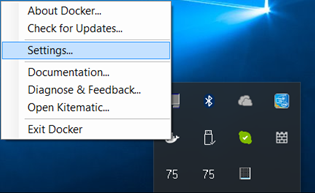
\includegraphics[width=0.3\textwidth]{mapContainerFolderWindows01.png}\end{center}}
	
	\item From the tab ``Shared Drives'', select the drive you want to make available to the containers, e.g., ``C'':
	\textbf{\begin{center}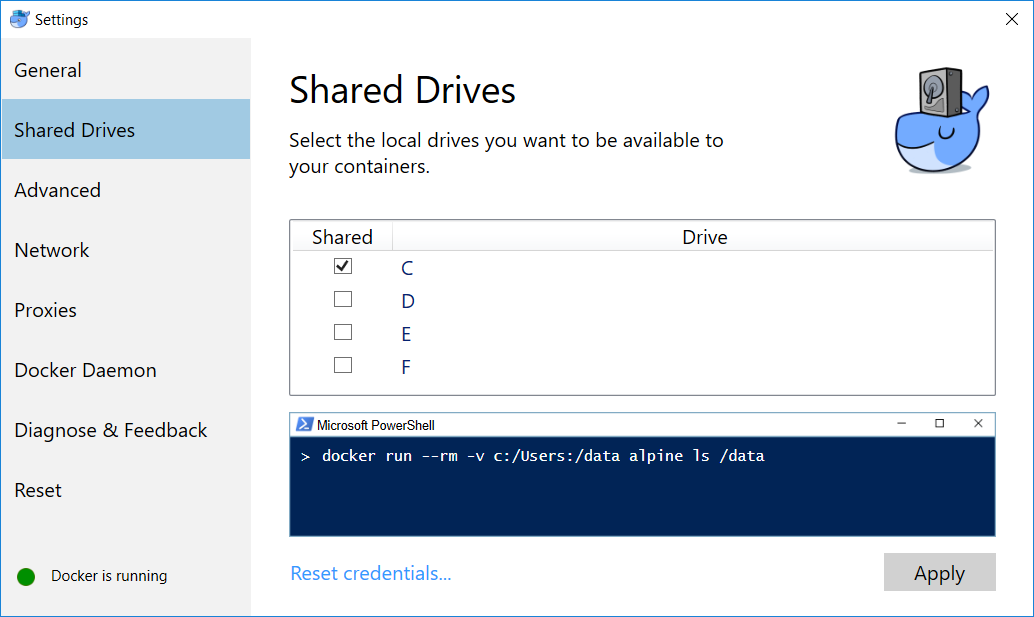
\includegraphics[width=0.6\textwidth]{mapContainerFolderWindows02.png}\end{center}}
	
	\item You will be prompted for login credentials to access the files:
	\textbf{\begin{center}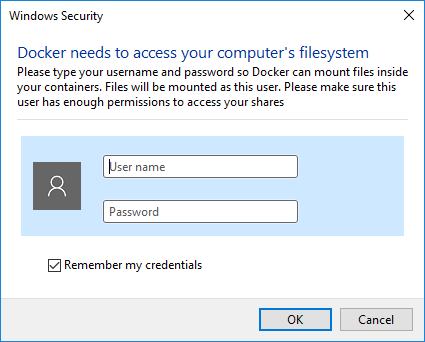
\includegraphics[width=0.6\textwidth]{mapContainerFolderWindows03.png}\end{center}}
	
	\item Start the container mounting the desired folder:
	{\VerbatimFont\begin{verbatim}$ docker run -v c:/Users/Dell/myresults:/data container_name ls /data\end{verbatim}}
	This command executes \identifier{ls /data} inside an instance of the container ``container\_name,'' after mounting ``\identifier{C:/Users/Dell/myresults/}'' into that path.
	
	\item The folder can be accessed normally from Windows and will reflect changes to any files automatically.
	\textbf{\begin{center}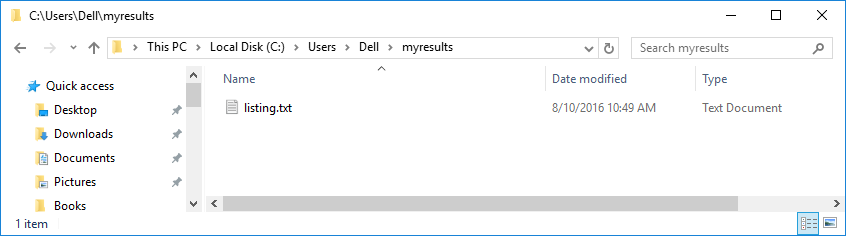
\includegraphics[width=0.6\textwidth]{mapContainerFolderWindows04.png}\end{center}}
\end{enumerate}


\end{appendices}


%------------------------------------------------------------%

\bibliographystyle{plain}
\bibliography{user_manual}

%------------------------------------------------------------%

%%% back page with a disclaimer, needed for any public document

\newpage
\makebackpage

\end{document}
